\chapter{Problem Space} \label{chap:probspace}

\section{The Focus}

%TODO why lossless important
%TODO why not lossy
%TODO why per read

It is important for fast parallel querying that the reads are compressed separately. That's not to say that each read is independent. Reads originating from the same channel and well/pore will have been recorded by the same sensor and so will likely have similar properties. This is especially true for reads recorded at a similar timestamp as each channel deteriorates over the course of a sequencing run. A compression method may take advantage of these available patterns but it is important for querying that each read can be decompressed independently. Perhaps there exists a multi-read compression strategy which is great for space reduction and hence archival purposes. However, such a strategy is not obvious and the primary desire of bioinformaticians is a better compression algorithm that does not sacrifice parallel querying. Hence, multi-read compression is outside the scope of this thesis.

Lossy compression, although an interesting avenue, is not desirable for most research applications where accuracy is more valued than storage space. For example, long-term archival of scholarly research data must be lossless to allow for public replication of any results. For this reason, lossless compression is the focus of this thesis.


\section{One Byte, Two Byte Exceptions}
\label{sec:vbbe21}
%\begin{figure}
%\centering
	\begin{tikzpicture}[node distance=0cm,start chain=1 going right] \footnotesize
  \tikzstyle{mytape}=[draw,minimum height=1.5cm]
	\node(A1)  [on chain=1,mytape,fill=blue!20] {$\underset{\text{exceptions}}{\underbrace{\overbracket{\text{ }e\text{ }}^{\text{2 bytes}}}_{\text{number of}}}$};
	\node(A2)  [on chain=1,mytape,fill=yellow!20] {$\underbrace{\overbracket{p_1,p_2,\dots,p_e}^{4e\text{ bytes}}}_{\text{exception positions}}$};
	\node(A3)  [on chain=1,mytape,fill=yellow!35] {$\underbrace{\overbracket{x_{p_1},x_{p_2},\dots,x_{p_e}}^{2e\text{ bytes}}}_{\text{two byte exceptions}}$};
	\node(A4)  [on chain=1,mytape,fill=green!35] {$\underbrace{\overbracket{x_{q_1},x_{q_2},\dots,x_{q_{n-e}}}^{n-e\text{ bytes}}}_{\text{one byte data}}$};
\end{tikzpicture}
%	\caption[The vbe21 encoding.]{\label{fig:vbe21} The vbe21 encoding takes two byte integers
%	$x_1,x_2,\dots,x_n$ and encodes those which cannot fit into one byte as
%	\textit{exceptions} at the beginning of the stream. There are $e$
%	exceptions which are recorded by their original positions
%	$p_1,p_2,\dots,p_e$ and values $x_{p_1},x_{p_2},\dots,x_{p_e}$.
%	Following this is the regular one byte data where $q_i$ is the original
%	position of the $i$-th one byte data point. This is beneficial when
%	there are few exceptions in the data.}
%\end{figure}


The one byte, two byte exceptions encoding, abbreviated to \textit{vbe21},
encodes a list of integers using one byte for each integer except for integers
which cannot fit into one byte, known as \textit{exceptions}, which are encoded
using two bytes. See Figure \ref{fig:vbe21}. Rather than using a control code to
mark where normal data and exceptions occur as in the Stream VByte codec
(Section \ref{subsubsec:svb}), the exceptions are encoded at the beginning since
it is expected that exceptions will occur with small probability.

The number of exceptions is written using 2 bytes, followed by the exceptions'
positions in the list using 4 bytes each, the exceptions themselves using 2
bytes each and finally the regular one byte data. For example, consider the
sequence of integers $1024,12,10,4096,0,1,2,1024$. There are three
exceptions 1024, 4096 and 1024. Hence, vbe21 would use
\[ 2 + 3(4+2) + 8-3 = 25 \]
bytes for this sequence. See Figure \ref{fig:vbe21-eg}.

\begin{figure}
\centering\begin{tikzpicture}[node distance=0cm,start chain=1 going right,start chain=2 going right] \footnotesize
  \tikzstyle{mytape}=[draw,minimum height=1.4cm]
    \node(A1)  [on chain=1,mytape,fill=blue!20] {$\underbrace{\overbracket{\texttt{0x00}|\texttt{0x03}}^{\text{2 bytes}}}_{3}$};
    \node(A2)  [on chain=1,mytape,fill=yellow!20] {$\underbrace{\overbracket{\texttt{0x00}|\texttt{0x00}|\texttt{0x00}|\texttt{0x00}}^{\text{4 bytes}}}_{0}$};
    \node(A3)  [on chain=1,mytape,fill=yellow!20] {$\underbrace{\overbracket{\texttt{0x00}|\texttt{0x00}|\texttt{0x00}|\texttt{0x03}}^{\text{4 bytes}}}_{3}$};
    \node(A4)  [on chain=1,mytape,fill=yellow!20] {$\underbrace{\overbracket{\texttt{0x00}|\texttt{0x00}|\texttt{0x00}|\texttt{0x07}}^{\text{4 bytes}}}_{7}$};
    \node(B1)  [on chain=2,mytape,fill=yellow!35,below of=A1,node distance=1.4cm] {$\underbrace{\overbracket{\texttt{0x04}|\texttt{0x00}}^{\text{2 bytes}}}_{1024}$};
    \node(B2)  [on chain=2,mytape,fill=yellow!35] {$\underbrace{\overbracket{\texttt{0x10}|\texttt{0x00}}^{\text{2 bytes}}}_{\num{4096}}$};
    \node(B3)  [on chain=2,mytape,fill=yellow!35] {$\underbrace{\overbracket{\texttt{0x04}|\texttt{0x00}}^{\text{2 bytes}}}_{1024}$};
    \node(B4)  [on chain=2,mytape,fill=green!35] {$\underbrace{\overbracket{\texttt{0x0c}}^{\text{1 byte}}}_{12}$};
    \node(B5)  [on chain=2,mytape,fill=green!35] {$\underbrace{\overbracket{\texttt{0x0a}}^{\text{1 byte}}}_{10}$};
    \node(B6)  [on chain=2,mytape,fill=green!35] {$\underbrace{\overbracket{\texttt{0x00}}^{\text{1 byte}}}_{0}$};
    \node(B7)  [on chain=2,mytape,fill=green!35] {$\underbrace{\overbracket{\texttt{0x01}}^{\text{1 byte}}}_{1}$};
    \node(B8)  [on chain=2,mytape,fill=green!35] {$\underbrace{\overbracket{\texttt{0x02}}^{\text{1 byte}}}_{2}$};
\end{tikzpicture}

	\caption[An example of $1024,12,10,4096, 0,1,2,1024$ encoded with vbe21.]{\label{fig:vbe21-eg} An example of $1024,12,10,4096,
	0,1,2,1024$ encoded with vbe21. The encoding order is read from left to
	right and top to bottom. There are 3 exceptions located at positions 0,
	3 and 7 with values 1024, 4096 and 1024. It uses 25 bytes in total.}
\end{figure}


Now, consider applying encoding $A$ to a read. Let $C_A:\Omega\to\mathbb{N}_0$
be a random variable measuring the resulting compressed size in bytes where
$\Omega$ is the space of possible nanopore reads. Then
\begin{align*}
	C_{vbe21} &= \text{exceptions} + \text{one byte data}\\
	&= (2 + 6X) + (N - X)\\
	&= 2 + 5X + N
\end{align*}
where $N$ and $X$ are random variables measuring the read length and number of
exceptions respectively. Recall from Section \ref{subsec:prob} that the
probability that a zig-zag delta is greater than 255 and therefore outside the one
byte range is $\sim 5\times 10^{-5}$ for the data. Thus, the expected number of
zig-zag delta exceptions is
\[ E[X] = (5 \times 10^{-5})E[N] \]
%Also, the read lengths can be modelled by the Gamma distribution $\Gamma(1.0885,0.0096)$.
where the expected read length is
\[ E[N] = 113471.4 \]
from Table \ref{tab:n}. So $E[X] \approx 5.67$, that is we expect roughly 5 to 6
exceptions per read when using the zig-zag delta transformation.
Then, the expected compressed size is given by
\begin{align*}
	E[C_{vbe21-zd}] &= 2 + (2.5\times 10^{-4})E[N]+ E[N]\\
	&= 2 + 1.00025E[N]\\
	&\approx 113502 \text{ bytes}
\end{align*}
where vbe21-zd means first apply the zig-zag delta encoding then vbe21. In
comparison, using the Stream VByte 16 (or \textit{svb16}) encoding, the
compressed size is given by
\begin{align*}
	C_{svb16} &= \lceil N/8 \rceil + 2X + (N - X)\\
	&= \lceil N/8 \rceil + X + N.
\end{align*}
Then, the expected compressed size is
\begin{align*}
	E[C_{svb16-zd}] &= \lceil E[N]/8 \rceil + (5 \times 10^{-5})E[N] + E[N]\\
	&= \lceil E[N]/8 \rceil + 1.00005E[N]\\
	&\approx 127661 \text{ bytes}\\
	&> E[C_{vbe21-zd}].
\end{align*}

This translates into roughly 8 bits per data point for vbe21-zd versus
9 for svb16-zd.
%See Table \ref{tab:vbe21-bpp}.
Intuitively these numbers make sense considering vbe21-zd essentially represents
most points using one byte each and svb16-zd stores one extra bit per point in
the control byte section.  Compare this to the entropy of the data which is 7.70
bits per point or 5.39 for the zig-zag deltas. So it is clear that
vbe21-zd saves more space than svb16-zd: roughly 14 KiB on average per read or
an estimated 6.6 GiB for the whole data set. However, this is merely a container
for the data which is useful for downstream compression; alone it doesn't
provide great compression results as is obvious when comparing it to the entropy
of the data.

vbe21-zd is linear in time complexity during encoding since it requires
applying the zig-zag delta transformation and checking which values are
exceptions. The same is true for decoding and the svb16-zd codec.

%\begin{table}
    \caption{\label{tab:vbe21-bpp} The theoretical expected bits per point for the
vbe21-zd and svb16-zd encodings.}
    \begin{tabular}{|l|l|}
        \hline
Encoding & Expected Bits Per Point\\
        \hline
vbe21-zd & 8\\
svb16-zd & 9\\
	\hline
    \end{tabular}
\end{table}


\subsection{Exceptions Encoding}

There are better ways of storing the exceptions than in the raw sequential
format of vbe21.
As we have seen there are usually 5 to 6 exceptions per read meaning that
storing the number of exceptions using two bytes which has a range of 0 to 65535
for all reads is wasteful.
In particular, the number of exceptions per read ranges from 0 to 3616 but 99\%
of reads have between 0 and 42 exceptions. See Table \ref{tab:ex}. Its
distribution, shown in Figure \ref{fig:nex-hist}, could be nicely fitted by an
exponential distribution. In fact, around 20\% of the reads have no exceptions
at all.

\begin{table}
    \caption{\label{tab:ex} Summary statistics of the number of exceptions per read and the zig-zag delta exceptions themselves in the data.}
	\begin{tabular}{|l|m{1.8cm}|l|}
	    \hline
	    Statistic & Number of Exceptions Per Read & Exceptions\\
        \hline
		Min &0 & 256\\
		Q1 & 1& 260\\

		Q2 & 3& 266\\
		Q3 & 6& 278\\
		Max & 3616& 2317\\
\hline
		Mean & 4.8546&277.0465\\
		Mode & 0&256\\
		SD & 18.0595&36.8207\\
	\hline
    \end{tabular}
\end{table}

\begin{figure}
	\centering
% Created by tikzDevice version 0.12.3.1 on 2022-10-11 18:23:57
% !TEX encoding = UTF-8 Unicode
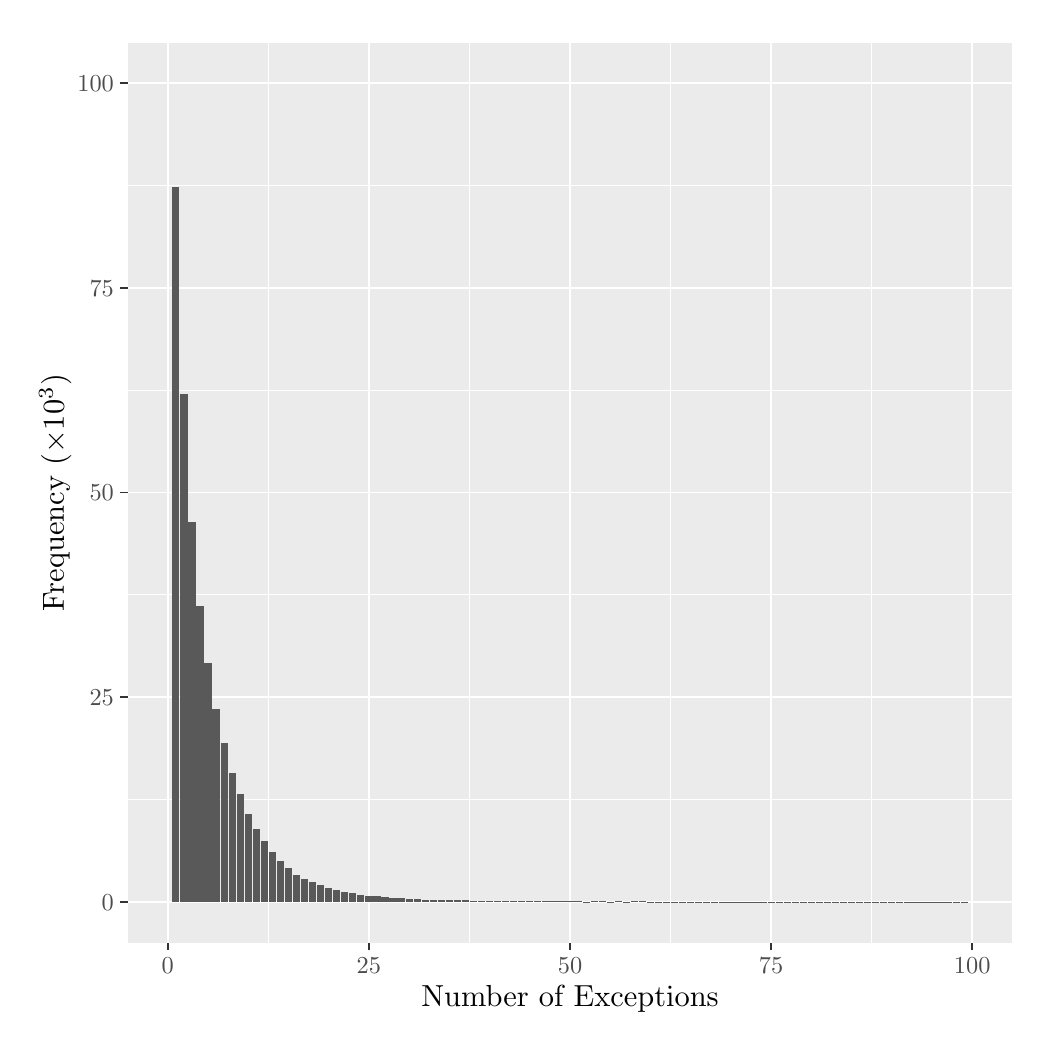
\begin{tikzpicture}[x=1pt,y=1pt]
\definecolor{fillColor}{RGB}{255,255,255}
\path[use as bounding box,fill=fillColor,fill opacity=0.00] (0,0) rectangle (361.35,361.35);
\begin{scope}
\path[clip] (  0.00,  0.00) rectangle (361.35,361.35);
\definecolor{drawColor}{RGB}{255,255,255}
\definecolor{fillColor}{RGB}{255,255,255}

\path[draw=drawColor,line width= 0.6pt,line join=round,line cap=round,fill=fillColor] (  0.00,  0.00) rectangle (361.35,361.35);
\end{scope}
\begin{scope}
\path[clip] ( 36.11, 30.69) rectangle (355.85,355.85);
\definecolor{fillColor}{gray}{0.92}

\path[fill=fillColor] ( 36.11, 30.69) rectangle (355.85,355.85);
\definecolor{drawColor}{RGB}{255,255,255}

\path[draw=drawColor,line width= 0.3pt,line join=round] ( 36.11, 82.45) --
	(355.85, 82.45);

\path[draw=drawColor,line width= 0.3pt,line join=round] ( 36.11,156.42) --
	(355.85,156.42);

\path[draw=drawColor,line width= 0.3pt,line join=round] ( 36.11,230.38) --
	(355.85,230.38);

\path[draw=drawColor,line width= 0.3pt,line join=round] ( 36.11,304.35) --
	(355.85,304.35);

\path[draw=drawColor,line width= 0.3pt,line join=round] ( 86.98, 30.69) --
	( 86.98,355.85);

\path[draw=drawColor,line width= 0.3pt,line join=round] (159.65, 30.69) --
	(159.65,355.85);

\path[draw=drawColor,line width= 0.3pt,line join=round] (232.31, 30.69) --
	(232.31,355.85);

\path[draw=drawColor,line width= 0.3pt,line join=round] (304.98, 30.69) --
	(304.98,355.85);

\path[draw=drawColor,line width= 0.6pt,line join=round] ( 36.11, 45.47) --
	(355.85, 45.47);

\path[draw=drawColor,line width= 0.6pt,line join=round] ( 36.11,119.43) --
	(355.85,119.43);

\path[draw=drawColor,line width= 0.6pt,line join=round] ( 36.11,193.40) --
	(355.85,193.40);

\path[draw=drawColor,line width= 0.6pt,line join=round] ( 36.11,267.37) --
	(355.85,267.37);

\path[draw=drawColor,line width= 0.6pt,line join=round] ( 36.11,341.34) --
	(355.85,341.34);

\path[draw=drawColor,line width= 0.6pt,line join=round] ( 50.64, 30.69) --
	( 50.64,355.85);

\path[draw=drawColor,line width= 0.6pt,line join=round] (123.31, 30.69) --
	(123.31,355.85);

\path[draw=drawColor,line width= 0.6pt,line join=round] (195.98, 30.69) --
	(195.98,355.85);

\path[draw=drawColor,line width= 0.6pt,line join=round] (268.65, 30.69) --
	(268.65,355.85);

\path[draw=drawColor,line width= 0.6pt,line join=round] (341.32, 30.69) --
	(341.32,355.85);
\definecolor{fillColor}{gray}{0.35}

\path[fill=fillColor] ( 52.24, 45.47) rectangle ( 54.86,303.76);

\path[fill=fillColor] ( 55.15, 45.47) rectangle ( 57.77,229.02);

\path[fill=fillColor] ( 58.06, 45.47) rectangle ( 60.67,182.55);

\path[fill=fillColor] ( 60.96, 45.47) rectangle ( 63.58,152.28);

\path[fill=fillColor] ( 63.87, 45.47) rectangle ( 66.49,131.71);

\path[fill=fillColor] ( 66.78, 45.47) rectangle ( 69.39,115.27);

\path[fill=fillColor] ( 69.68, 45.47) rectangle ( 72.30,103.03);

\path[fill=fillColor] ( 72.59, 45.47) rectangle ( 75.21, 92.15);

\path[fill=fillColor] ( 75.50, 45.47) rectangle ( 78.11, 84.47);

\path[fill=fillColor] ( 78.40, 45.47) rectangle ( 81.02, 77.36);

\path[fill=fillColor] ( 81.31, 45.47) rectangle ( 83.93, 71.87);

\path[fill=fillColor] ( 84.22, 45.47) rectangle ( 86.83, 67.43);

\path[fill=fillColor] ( 87.12, 45.47) rectangle ( 89.74, 63.64);

\path[fill=fillColor] ( 90.03, 45.47) rectangle ( 92.65, 60.19);

\path[fill=fillColor] ( 92.94, 45.47) rectangle ( 95.55, 57.70);

\path[fill=fillColor] ( 95.84, 45.47) rectangle ( 98.46, 55.08);

\path[fill=fillColor] ( 98.75, 45.47) rectangle (101.37, 53.84);

\path[fill=fillColor] (101.66, 45.47) rectangle (104.27, 52.65);

\path[fill=fillColor] (104.56, 45.47) rectangle (107.18, 51.51);

\path[fill=fillColor] (107.47, 45.47) rectangle (110.09, 50.42);

\path[fill=fillColor] (110.38, 45.47) rectangle (112.99, 49.62);

\path[fill=fillColor] (113.28, 45.47) rectangle (115.90, 48.95);

\path[fill=fillColor] (116.19, 45.47) rectangle (118.81, 48.54);

\path[fill=fillColor] (119.10, 45.47) rectangle (121.71, 48.05);

\path[fill=fillColor] (122.00, 45.47) rectangle (124.62, 47.58);

\path[fill=fillColor] (124.91, 45.47) rectangle (127.53, 47.40);

\path[fill=fillColor] (127.82, 45.47) rectangle (130.43, 47.26);

\path[fill=fillColor] (130.72, 45.47) rectangle (133.34, 46.87);

\path[fill=fillColor] (133.63, 45.47) rectangle (136.25, 46.79);

\path[fill=fillColor] (136.54, 45.47) rectangle (139.15, 46.48);

\path[fill=fillColor] (139.44, 45.47) rectangle (142.06, 46.53);

\path[fill=fillColor] (142.35, 45.47) rectangle (144.97, 46.31);

\path[fill=fillColor] (145.26, 45.47) rectangle (147.87, 46.29);

\path[fill=fillColor] (148.17, 45.47) rectangle (150.78, 46.20);

\path[fill=fillColor] (151.07, 45.47) rectangle (153.69, 46.11);

\path[fill=fillColor] (153.98, 45.47) rectangle (156.59, 45.98);

\path[fill=fillColor] (156.89, 45.47) rectangle (159.50, 46.01);

\path[fill=fillColor] (159.79, 45.47) rectangle (162.41, 45.94);

\path[fill=fillColor] (162.70, 45.47) rectangle (165.31, 45.80);

\path[fill=fillColor] (165.61, 45.47) rectangle (168.22, 45.91);

\path[fill=fillColor] (168.51, 45.47) rectangle (171.13, 45.81);

\path[fill=fillColor] (171.42, 45.47) rectangle (174.03, 45.73);

\path[fill=fillColor] (174.33, 45.47) rectangle (176.94, 45.84);

\path[fill=fillColor] (177.23, 45.47) rectangle (179.85, 45.73);

\path[fill=fillColor] (180.14, 45.47) rectangle (182.76, 45.74);

\path[fill=fillColor] (183.05, 45.47) rectangle (185.66, 45.74);

\path[fill=fillColor] (185.95, 45.47) rectangle (188.57, 45.67);

\path[fill=fillColor] (188.86, 45.47) rectangle (191.48, 45.69);

\path[fill=fillColor] (191.77, 45.47) rectangle (194.38, 45.65);

\path[fill=fillColor] (194.67, 45.47) rectangle (197.29, 45.68);

\path[fill=fillColor] (197.58, 45.47) rectangle (200.20, 45.71);

\path[fill=fillColor] (200.49, 45.47) rectangle (203.10, 45.59);

\path[fill=fillColor] (203.39, 45.47) rectangle (206.01, 45.66);

\path[fill=fillColor] (206.30, 45.47) rectangle (208.92, 45.63);

\path[fill=fillColor] (209.21, 45.47) rectangle (211.82, 45.59);

\path[fill=fillColor] (212.11, 45.47) rectangle (214.73, 45.60);

\path[fill=fillColor] (215.02, 45.47) rectangle (217.64, 45.58);

\path[fill=fillColor] (217.93, 45.47) rectangle (220.54, 45.62);

\path[fill=fillColor] (220.83, 45.47) rectangle (223.45, 45.60);

\path[fill=fillColor] (223.74, 45.47) rectangle (226.36, 45.55);

\path[fill=fillColor] (226.65, 45.47) rectangle (229.26, 45.57);

\path[fill=fillColor] (229.55, 45.47) rectangle (232.17, 45.55);

\path[fill=fillColor] (232.46, 45.47) rectangle (235.08, 45.56);

\path[fill=fillColor] (235.37, 45.47) rectangle (237.98, 45.56);

\path[fill=fillColor] (238.27, 45.47) rectangle (240.89, 45.55);

\path[fill=fillColor] (241.18, 45.47) rectangle (243.80, 45.52);

\path[fill=fillColor] (244.09, 45.47) rectangle (246.70, 45.53);

\path[fill=fillColor] (246.99, 45.47) rectangle (249.61, 45.57);

\path[fill=fillColor] (249.90, 45.47) rectangle (252.52, 45.54);

\path[fill=fillColor] (252.81, 45.47) rectangle (255.42, 45.54);

\path[fill=fillColor] (255.71, 45.47) rectangle (258.33, 45.53);

\path[fill=fillColor] (258.62, 45.47) rectangle (261.24, 45.51);

\path[fill=fillColor] (261.53, 45.47) rectangle (264.14, 45.53);

\path[fill=fillColor] (264.43, 45.47) rectangle (267.05, 45.50);

\path[fill=fillColor] (267.34, 45.47) rectangle (269.96, 45.52);

\path[fill=fillColor] (270.25, 45.47) rectangle (272.86, 45.53);

\path[fill=fillColor] (273.15, 45.47) rectangle (275.77, 45.53);

\path[fill=fillColor] (276.06, 45.47) rectangle (278.68, 45.51);

\path[fill=fillColor] (278.97, 45.47) rectangle (281.58, 45.53);

\path[fill=fillColor] (281.87, 45.47) rectangle (284.49, 45.53);

\path[fill=fillColor] (284.78, 45.47) rectangle (287.40, 45.50);

\path[fill=fillColor] (287.69, 45.47) rectangle (290.30, 45.50);

\path[fill=fillColor] (290.59, 45.47) rectangle (293.21, 45.49);

\path[fill=fillColor] (293.50, 45.47) rectangle (296.12, 45.51);

\path[fill=fillColor] (296.41, 45.47) rectangle (299.02, 45.50);

\path[fill=fillColor] (299.31, 45.47) rectangle (301.93, 45.53);

\path[fill=fillColor] (302.22, 45.47) rectangle (304.84, 45.51);

\path[fill=fillColor] (305.13, 45.47) rectangle (307.74, 45.51);

\path[fill=fillColor] (308.03, 45.47) rectangle (310.65, 45.51);

\path[fill=fillColor] (310.94, 45.47) rectangle (313.56, 45.50);

\path[fill=fillColor] (313.85, 45.47) rectangle (316.46, 45.50);

\path[fill=fillColor] (316.75, 45.47) rectangle (319.37, 45.53);

\path[fill=fillColor] (319.66, 45.47) rectangle (322.28, 45.50);

\path[fill=fillColor] (322.57, 45.47) rectangle (325.18, 45.50);

\path[fill=fillColor] (325.47, 45.47) rectangle (328.09, 45.51);

\path[fill=fillColor] (328.38, 45.47) rectangle (331.00, 45.50);

\path[fill=fillColor] (331.29, 45.47) rectangle (333.90, 45.51);

\path[fill=fillColor] (334.19, 45.47) rectangle (336.81, 45.50);

\path[fill=fillColor] (337.10, 45.47) rectangle (339.72, 45.49);
\end{scope}
\begin{scope}
\path[clip] (  0.00,  0.00) rectangle (361.35,361.35);
\definecolor{drawColor}{gray}{0.30}

\node[text=drawColor,anchor=base east,inner sep=0pt, outer sep=0pt, scale=  0.88] at ( 31.16, 42.44) {0};

\node[text=drawColor,anchor=base east,inner sep=0pt, outer sep=0pt, scale=  0.88] at ( 31.16,116.40) {25};

\node[text=drawColor,anchor=base east,inner sep=0pt, outer sep=0pt, scale=  0.88] at ( 31.16,190.37) {50};

\node[text=drawColor,anchor=base east,inner sep=0pt, outer sep=0pt, scale=  0.88] at ( 31.16,264.34) {75};

\node[text=drawColor,anchor=base east,inner sep=0pt, outer sep=0pt, scale=  0.88] at ( 31.16,338.31) {100};
\end{scope}
\begin{scope}
\path[clip] (  0.00,  0.00) rectangle (361.35,361.35);
\definecolor{drawColor}{gray}{0.20}

\path[draw=drawColor,line width= 0.6pt,line join=round] ( 33.36, 45.47) --
	( 36.11, 45.47);

\path[draw=drawColor,line width= 0.6pt,line join=round] ( 33.36,119.43) --
	( 36.11,119.43);

\path[draw=drawColor,line width= 0.6pt,line join=round] ( 33.36,193.40) --
	( 36.11,193.40);

\path[draw=drawColor,line width= 0.6pt,line join=round] ( 33.36,267.37) --
	( 36.11,267.37);

\path[draw=drawColor,line width= 0.6pt,line join=round] ( 33.36,341.34) --
	( 36.11,341.34);
\end{scope}
\begin{scope}
\path[clip] (  0.00,  0.00) rectangle (361.35,361.35);
\definecolor{drawColor}{gray}{0.20}

\path[draw=drawColor,line width= 0.6pt,line join=round] ( 50.64, 27.94) --
	( 50.64, 30.69);

\path[draw=drawColor,line width= 0.6pt,line join=round] (123.31, 27.94) --
	(123.31, 30.69);

\path[draw=drawColor,line width= 0.6pt,line join=round] (195.98, 27.94) --
	(195.98, 30.69);

\path[draw=drawColor,line width= 0.6pt,line join=round] (268.65, 27.94) --
	(268.65, 30.69);

\path[draw=drawColor,line width= 0.6pt,line join=round] (341.32, 27.94) --
	(341.32, 30.69);
\end{scope}
\begin{scope}
\path[clip] (  0.00,  0.00) rectangle (361.35,361.35);
\definecolor{drawColor}{gray}{0.30}

\node[text=drawColor,anchor=base,inner sep=0pt, outer sep=0pt, scale=  0.88] at ( 50.64, 19.68) {0};

\node[text=drawColor,anchor=base,inner sep=0pt, outer sep=0pt, scale=  0.88] at (123.31, 19.68) {25};

\node[text=drawColor,anchor=base,inner sep=0pt, outer sep=0pt, scale=  0.88] at (195.98, 19.68) {50};

\node[text=drawColor,anchor=base,inner sep=0pt, outer sep=0pt, scale=  0.88] at (268.65, 19.68) {75};

\node[text=drawColor,anchor=base,inner sep=0pt, outer sep=0pt, scale=  0.88] at (341.32, 19.68) {100};
\end{scope}
\begin{scope}
\path[clip] (  0.00,  0.00) rectangle (361.35,361.35);
\definecolor{drawColor}{RGB}{0,0,0}

\node[text=drawColor,anchor=base,inner sep=0pt, outer sep=0pt, scale=  1.10] at (195.98,  7.64) {Number of Exceptions};
\end{scope}
\begin{scope}
\path[clip] (  0.00,  0.00) rectangle (361.35,361.35);
\definecolor{drawColor}{RGB}{0,0,0}

\node[text=drawColor,rotate= 90.00,anchor=base,inner sep=0pt, outer sep=0pt, scale=  1.10] at ( 13.08,193.27) {Frequency ($\times 10^3$)};
\end{scope}
\end{tikzpicture}

	\caption{\label{fig:nex-hist}Histogram of the number of exceptions per read up to 100 which appears to nicely follow an exponential distribution. Values after 100 occur highly infrequently -- there are only 546 out of \num{500000} reads with more than 100 exceptions.}
\end{figure}


Instead of storing two bytes for the number of exceptions we can bit pack the
number of exceptions using four bits to represent the number of bits used.
Refer back to Section \ref{sec:bitpack} for a review of bit packing.
The maximum number of exceptions, 3616, requires at least
12 bits to represent it. Using the bit packing approach, $4+12=16$ bits or two
bytes would be used to represent it -- which is equivalent to the naive
approach. That is, in the worst case bit packing use the same space as the naive
approach. In the best case when there are zero exceptions only four bits are
required, and as long as there are lesser than 16 exceptions up to one byte is
used. Although this approach clearly saves space, we are talking about saving at
most 12 bits which is miniscule compared to the scale of the data.

Similarly, we can store the exceptions' data in a more compact form.
The exceptions themselves range from 256 to 2317 but 99\%
of the exceptions do not go higher than 481. The mean and mode are $\sim$277 and
256 respectively. Refer to Table \ref{tab:ex} for a summary and Figure
\ref{fig:ex-hist} for the histogram. Notably, the frequency of even-numbered
exceptions is much greater than adjacent odd-numbered exceptions from 256 up to
$\sim$330. This is due to large positive deltas occuring more frequently than
large negative deltas as previously discussed in Section \ref{subsec:stripe}.
One simple approach to encoding the exceptions is to subtract 256 since this is
the minimum exception value and then apply bit packing using 4 bits as before. The
average exception can then be represented using
0 to 5 bits which is better than the naive 16-bit per exception encoding. This
results in an expected improvement of $(16-5)\times 5-4=51$ bits per read.
In the worst case, the number of bits used per exception for this data will be 12
or $4 + 12e$ in total, which is better than the naive approach for $e>1$ and
equivalent for $e=1$. The implications of this is that bit packing the
exceptions' data never consumes more space than the naive strategy.

\begin{figure}
	\centering
% Created by tikzDevice version 0.12.3.1 on 2022-10-11 17:28:28
% !TEX encoding = UTF-8 Unicode
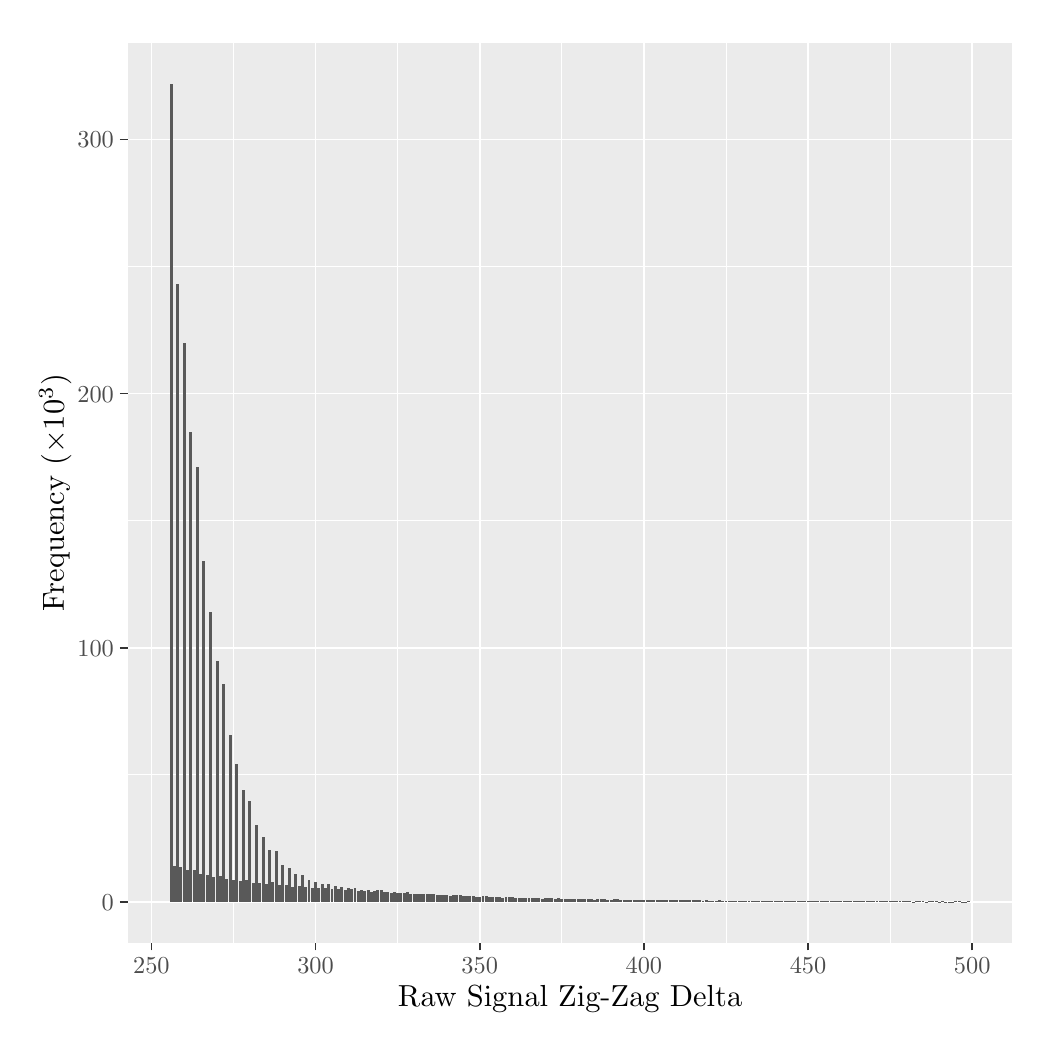
\begin{tikzpicture}[x=1pt,y=1pt]
\definecolor{fillColor}{RGB}{255,255,255}
\path[use as bounding box,fill=fillColor,fill opacity=0.00] (0,0) rectangle (361.35,361.35);
\begin{scope}
\path[clip] (  0.00,  0.00) rectangle (361.35,361.35);
\definecolor{drawColor}{RGB}{255,255,255}
\definecolor{fillColor}{RGB}{255,255,255}

\path[draw=drawColor,line width= 0.6pt,line join=round,line cap=round,fill=fillColor] (  0.00,  0.00) rectangle (361.35,361.35);
\end{scope}
\begin{scope}
\path[clip] ( 36.11, 30.69) rectangle (355.85,355.85);
\definecolor{fillColor}{gray}{0.92}

\path[fill=fillColor] ( 36.11, 30.69) rectangle (355.85,355.85);
\definecolor{drawColor}{RGB}{255,255,255}

\path[draw=drawColor,line width= 0.3pt,line join=round] ( 36.11, 91.37) --
	(355.85, 91.37);

\path[draw=drawColor,line width= 0.3pt,line join=round] ( 36.11,183.19) --
	(355.85,183.19);

\path[draw=drawColor,line width= 0.3pt,line join=round] ( 36.11,275.01) --
	(355.85,275.01);

\path[draw=drawColor,line width= 0.3pt,line join=round] ( 74.37, 30.69) --
	( 74.37,355.85);

\path[draw=drawColor,line width= 0.3pt,line join=round] (133.69, 30.69) --
	(133.69,355.85);

\path[draw=drawColor,line width= 0.3pt,line join=round] (193.01, 30.69) --
	(193.01,355.85);

\path[draw=drawColor,line width= 0.3pt,line join=round] (252.34, 30.69) --
	(252.34,355.85);

\path[draw=drawColor,line width= 0.3pt,line join=round] (311.66, 30.69) --
	(311.66,355.85);

\path[draw=drawColor,line width= 0.6pt,line join=round] ( 36.11, 45.47) --
	(355.85, 45.47);

\path[draw=drawColor,line width= 0.6pt,line join=round] ( 36.11,137.28) --
	(355.85,137.28);

\path[draw=drawColor,line width= 0.6pt,line join=round] ( 36.11,229.10) --
	(355.85,229.10);

\path[draw=drawColor,line width= 0.6pt,line join=round] ( 36.11,320.91) --
	(355.85,320.91);

\path[draw=drawColor,line width= 0.6pt,line join=round] ( 44.71, 30.69) --
	( 44.71,355.85);

\path[draw=drawColor,line width= 0.6pt,line join=round] (104.03, 30.69) --
	(104.03,355.85);

\path[draw=drawColor,line width= 0.6pt,line join=round] (163.35, 30.69) --
	(163.35,355.85);

\path[draw=drawColor,line width= 0.6pt,line join=round] (222.67, 30.69) --
	(222.67,355.85);

\path[draw=drawColor,line width= 0.6pt,line join=round] (282.00, 30.69) --
	(282.00,355.85);

\path[draw=drawColor,line width= 0.6pt,line join=round] (341.32, 30.69) --
	(341.32,355.85);
\definecolor{fillColor}{gray}{0.35}

\path[fill=fillColor] ( 51.30, 45.47) rectangle ( 52.37,341.07);

\path[fill=fillColor] ( 52.48, 45.47) rectangle ( 53.55, 58.32);

\path[fill=fillColor] ( 53.67, 45.47) rectangle ( 54.74,268.74);

\path[fill=fillColor] ( 54.86, 45.47) rectangle ( 55.92, 58.08);

\path[fill=fillColor] ( 56.04, 45.47) rectangle ( 57.11,247.36);

\path[fill=fillColor] ( 57.23, 45.47) rectangle ( 58.30, 56.94);

\path[fill=fillColor] ( 58.42, 45.47) rectangle ( 59.48,215.13);

\path[fill=fillColor] ( 59.60, 45.47) rectangle ( 60.67, 57.07);

\path[fill=fillColor] ( 60.79, 45.47) rectangle ( 61.86,202.50);

\path[fill=fillColor] ( 61.98, 45.47) rectangle ( 63.04, 55.42);

\path[fill=fillColor] ( 63.16, 45.47) rectangle ( 64.23,168.69);

\path[fill=fillColor] ( 64.35, 45.47) rectangle ( 65.42, 55.18);

\path[fill=fillColor] ( 65.53, 45.47) rectangle ( 66.60,150.14);

\path[fill=fillColor] ( 66.72, 45.47) rectangle ( 67.79, 54.37);

\path[fill=fillColor] ( 67.91, 45.47) rectangle ( 68.97,132.62);

\path[fill=fillColor] ( 69.09, 45.47) rectangle ( 70.16, 54.86);

\path[fill=fillColor] ( 70.28, 45.47) rectangle ( 71.35,124.30);

\path[fill=fillColor] ( 71.47, 45.47) rectangle ( 72.53, 53.65);

\path[fill=fillColor] ( 72.65, 45.47) rectangle ( 73.72,105.80);

\path[fill=fillColor] ( 73.84, 45.47) rectangle ( 74.91, 53.53);

\path[fill=fillColor] ( 75.03, 45.47) rectangle ( 76.09, 95.30);

\path[fill=fillColor] ( 76.21, 45.47) rectangle ( 77.28, 53.03);

\path[fill=fillColor] ( 77.40, 45.47) rectangle ( 78.47, 85.80);

\path[fill=fillColor] ( 78.58, 45.47) rectangle ( 79.65, 53.38);

\path[fill=fillColor] ( 79.77, 45.47) rectangle ( 80.84, 81.94);

\path[fill=fillColor] ( 80.96, 45.47) rectangle ( 82.03, 52.23);

\path[fill=fillColor] ( 82.14, 45.47) rectangle ( 83.21, 73.06);

\path[fill=fillColor] ( 83.33, 45.47) rectangle ( 84.40, 52.19);

\path[fill=fillColor] ( 84.52, 45.47) rectangle ( 85.58, 68.84);

\path[fill=fillColor] ( 85.70, 45.47) rectangle ( 86.77, 51.88);

\path[fill=fillColor] ( 86.89, 45.47) rectangle ( 87.96, 64.21);

\path[fill=fillColor] ( 88.08, 45.47) rectangle ( 89.14, 52.55);

\path[fill=fillColor] ( 89.26, 45.47) rectangle ( 90.33, 63.73);

\path[fill=fillColor] ( 90.45, 45.47) rectangle ( 91.52, 51.52);

\path[fill=fillColor] ( 91.64, 45.47) rectangle ( 92.70, 58.82);

\path[fill=fillColor] ( 92.82, 45.47) rectangle ( 93.89, 51.40);

\path[fill=fillColor] ( 94.01, 45.47) rectangle ( 95.08, 57.60);

\path[fill=fillColor] ( 95.19, 45.47) rectangle ( 96.26, 51.00);

\path[fill=fillColor] ( 96.38, 45.47) rectangle ( 97.45, 55.59);

\path[fill=fillColor] ( 97.57, 45.47) rectangle ( 98.64, 51.22);

\path[fill=fillColor] ( 98.75, 45.47) rectangle ( 99.82, 55.06);

\path[fill=fillColor] ( 99.94, 45.47) rectangle (101.01, 50.82);

\path[fill=fillColor] (101.13, 45.47) rectangle (102.19, 53.45);

\path[fill=fillColor] (102.31, 45.47) rectangle (103.38, 50.61);

\path[fill=fillColor] (103.50, 45.47) rectangle (104.57, 52.63);

\path[fill=fillColor] (104.69, 45.47) rectangle (105.75, 50.39);

\path[fill=fillColor] (105.87, 45.47) rectangle (106.94, 52.08);

\path[fill=fillColor] (107.06, 45.47) rectangle (108.13, 50.65);

\path[fill=fillColor] (108.25, 45.47) rectangle (109.31, 52.00);

\path[fill=fillColor] (109.43, 45.47) rectangle (110.50, 50.26);

\path[fill=fillColor] (110.62, 45.47) rectangle (111.69, 51.13);

\path[fill=fillColor] (111.80, 45.47) rectangle (112.87, 50.05);

\path[fill=fillColor] (112.99, 45.47) rectangle (114.06, 50.72);

\path[fill=fillColor] (114.18, 45.47) rectangle (115.25, 49.84);

\path[fill=fillColor] (115.36, 45.47) rectangle (116.43, 50.38);

\path[fill=fillColor] (116.55, 45.47) rectangle (117.62, 50.03);

\path[fill=fillColor] (117.74, 45.47) rectangle (118.80, 50.45);

\path[fill=fillColor] (118.92, 45.47) rectangle (119.99, 49.53);

\path[fill=fillColor] (120.11, 45.47) rectangle (121.18, 49.83);

\path[fill=fillColor] (121.30, 45.47) rectangle (122.36, 49.34);

\path[fill=fillColor] (122.48, 45.47) rectangle (123.55, 49.74);

\path[fill=fillColor] (123.67, 45.47) rectangle (124.74, 49.20);

\path[fill=fillColor] (124.86, 45.47) rectangle (125.92, 49.39);

\path[fill=fillColor] (126.04, 45.47) rectangle (127.11, 49.63);

\path[fill=fillColor] (127.23, 45.47) rectangle (128.30, 49.72);

\path[fill=fillColor] (128.41, 45.47) rectangle (129.48, 48.89);

\path[fill=fillColor] (129.60, 45.47) rectangle (130.67, 49.02);

\path[fill=fillColor] (130.79, 45.47) rectangle (131.85, 48.70);

\path[fill=fillColor] (131.97, 45.47) rectangle (133.04, 49.02);

\path[fill=fillColor] (133.16, 45.47) rectangle (134.23, 48.56);

\path[fill=fillColor] (134.35, 45.47) rectangle (135.41, 48.63);

\path[fill=fillColor] (135.53, 45.47) rectangle (136.60, 48.78);

\path[fill=fillColor] (136.72, 45.47) rectangle (137.79, 48.94);

\path[fill=fillColor] (137.91, 45.47) rectangle (138.97, 48.45);

\path[fill=fillColor] (139.09, 45.47) rectangle (140.16, 48.45);

\path[fill=fillColor] (140.28, 45.47) rectangle (141.35, 48.29);

\path[fill=fillColor] (141.46, 45.47) rectangle (142.53, 48.26);

\path[fill=fillColor] (142.65, 45.47) rectangle (143.72, 48.14);

\path[fill=fillColor] (143.84, 45.47) rectangle (144.91, 48.13);

\path[fill=fillColor] (145.02, 45.47) rectangle (146.09, 48.21);

\path[fill=fillColor] (146.21, 45.47) rectangle (147.28, 48.16);

\path[fill=fillColor] (147.40, 45.47) rectangle (148.46, 47.87);

\path[fill=fillColor] (148.58, 45.47) rectangle (149.65, 48.02);

\path[fill=fillColor] (149.77, 45.47) rectangle (150.84, 47.77);

\path[fill=fillColor] (150.96, 45.47) rectangle (152.02, 47.92);

\path[fill=fillColor] (152.14, 45.47) rectangle (153.21, 47.64);

\path[fill=fillColor] (153.33, 45.47) rectangle (154.40, 47.79);

\path[fill=fillColor] (154.52, 45.47) rectangle (155.58, 47.79);

\path[fill=fillColor] (155.70, 45.47) rectangle (156.77, 47.87);

\path[fill=fillColor] (156.89, 45.47) rectangle (157.96, 47.41);

\path[fill=fillColor] (158.07, 45.47) rectangle (159.14, 47.60);

\path[fill=fillColor] (159.26, 45.47) rectangle (160.33, 47.45);

\path[fill=fillColor] (160.45, 45.47) rectangle (161.52, 47.53);

\path[fill=fillColor] (161.63, 45.47) rectangle (162.70, 47.28);

\path[fill=fillColor] (162.82, 45.47) rectangle (163.89, 47.36);

\path[fill=fillColor] (164.01, 45.47) rectangle (165.07, 47.44);

\path[fill=fillColor] (165.19, 45.47) rectangle (166.26, 47.53);

\path[fill=fillColor] (166.38, 45.47) rectangle (167.45, 47.16);

\path[fill=fillColor] (167.57, 45.47) rectangle (168.63, 47.28);

\path[fill=fillColor] (168.75, 45.47) rectangle (169.82, 47.08);

\path[fill=fillColor] (169.94, 45.47) rectangle (171.01, 47.23);

\path[fill=fillColor] (171.13, 45.47) rectangle (172.19, 47.01);

\path[fill=fillColor] (172.31, 45.47) rectangle (173.38, 47.12);

\path[fill=fillColor] (173.50, 45.47) rectangle (174.57, 47.07);

\path[fill=fillColor] (174.68, 45.47) rectangle (175.75, 47.10);

\path[fill=fillColor] (175.87, 45.47) rectangle (176.94, 46.90);

\path[fill=fillColor] (177.06, 45.47) rectangle (178.13, 46.95);

\path[fill=fillColor] (178.24, 45.47) rectangle (179.31, 46.84);

\path[fill=fillColor] (179.43, 45.47) rectangle (180.50, 46.93);

\path[fill=fillColor] (180.62, 45.47) rectangle (181.68, 46.77);

\path[fill=fillColor] (181.80, 45.47) rectangle (182.87, 46.83);

\path[fill=fillColor] (182.99, 45.47) rectangle (184.06, 46.79);

\path[fill=fillColor] (184.18, 45.47) rectangle (185.24, 46.87);

\path[fill=fillColor] (185.36, 45.47) rectangle (186.43, 46.66);

\path[fill=fillColor] (186.55, 45.47) rectangle (187.62, 46.70);

\path[fill=fillColor] (187.74, 45.47) rectangle (188.80, 46.69);

\path[fill=fillColor] (188.92, 45.47) rectangle (189.99, 46.71);

\path[fill=fillColor] (190.11, 45.47) rectangle (191.18, 46.63);

\path[fill=fillColor] (191.29, 45.47) rectangle (192.36, 46.68);

\path[fill=fillColor] (192.48, 45.47) rectangle (193.55, 46.65);

\path[fill=fillColor] (193.67, 45.47) rectangle (194.73, 46.63);

\path[fill=fillColor] (194.85, 45.47) rectangle (195.92, 46.46);

\path[fill=fillColor] (196.04, 45.47) rectangle (197.11, 46.51);

\path[fill=fillColor] (197.23, 45.47) rectangle (198.29, 46.47);

\path[fill=fillColor] (198.41, 45.47) rectangle (199.48, 46.48);

\path[fill=fillColor] (199.60, 45.47) rectangle (200.67, 46.41);

\path[fill=fillColor] (200.79, 45.47) rectangle (201.85, 46.41);

\path[fill=fillColor] (201.97, 45.47) rectangle (203.04, 46.48);

\path[fill=fillColor] (203.16, 45.47) rectangle (204.23, 46.55);

\path[fill=fillColor] (204.34, 45.47) rectangle (205.41, 46.29);

\path[fill=fillColor] (205.53, 45.47) rectangle (206.60, 46.39);

\path[fill=fillColor] (206.72, 45.47) rectangle (207.79, 46.33);

\path[fill=fillColor] (207.90, 45.47) rectangle (208.97, 46.36);

\path[fill=fillColor] (209.09, 45.47) rectangle (210.16, 46.31);

\path[fill=fillColor] (210.28, 45.47) rectangle (211.34, 46.30);

\path[fill=fillColor] (211.46, 45.47) rectangle (212.53, 46.36);

\path[fill=fillColor] (212.65, 45.47) rectangle (213.72, 46.35);

\path[fill=fillColor] (213.84, 45.47) rectangle (214.90, 46.19);

\path[fill=fillColor] (215.02, 45.47) rectangle (216.09, 46.23);

\path[fill=fillColor] (216.21, 45.47) rectangle (217.28, 46.21);

\path[fill=fillColor] (217.40, 45.47) rectangle (218.46, 46.19);

\path[fill=fillColor] (218.58, 45.47) rectangle (219.65, 46.21);

\path[fill=fillColor] (219.77, 45.47) rectangle (220.84, 46.18);

\path[fill=fillColor] (220.95, 45.47) rectangle (222.02, 46.17);

\path[fill=fillColor] (222.14, 45.47) rectangle (223.21, 46.19);

\path[fill=fillColor] (223.33, 45.47) rectangle (224.40, 46.18);

\path[fill=fillColor] (224.51, 45.47) rectangle (225.58, 46.12);

\path[fill=fillColor] (225.70, 45.47) rectangle (226.77, 46.08);

\path[fill=fillColor] (226.89, 45.47) rectangle (227.95, 46.10);

\path[fill=fillColor] (228.07, 45.47) rectangle (229.14, 46.09);

\path[fill=fillColor] (229.26, 45.47) rectangle (230.33, 46.07);

\path[fill=fillColor] (230.45, 45.47) rectangle (231.51, 46.13);

\path[fill=fillColor] (231.63, 45.47) rectangle (232.70, 46.04);

\path[fill=fillColor] (232.82, 45.47) rectangle (233.89, 46.04);

\path[fill=fillColor] (234.01, 45.47) rectangle (235.07, 45.98);

\path[fill=fillColor] (235.19, 45.47) rectangle (236.26, 46.03);

\path[fill=fillColor] (236.38, 45.47) rectangle (237.45, 45.97);

\path[fill=fillColor] (237.56, 45.47) rectangle (238.63, 46.03);

\path[fill=fillColor] (238.75, 45.47) rectangle (239.82, 45.99);

\path[fill=fillColor] (239.94, 45.47) rectangle (241.01, 46.09);

\path[fill=fillColor] (241.12, 45.47) rectangle (242.19, 46.03);

\path[fill=fillColor] (242.31, 45.47) rectangle (243.38, 45.97);

\path[fill=fillColor] (243.50, 45.47) rectangle (244.56, 45.91);

\path[fill=fillColor] (244.68, 45.47) rectangle (245.75, 46.00);

\path[fill=fillColor] (245.87, 45.47) rectangle (246.94, 45.90);

\path[fill=fillColor] (247.06, 45.47) rectangle (248.12, 45.93);

\path[fill=fillColor] (248.24, 45.47) rectangle (249.31, 45.86);

\path[fill=fillColor] (249.43, 45.47) rectangle (250.50, 45.96);

\path[fill=fillColor] (250.61, 45.47) rectangle (251.68, 45.90);

\path[fill=fillColor] (251.80, 45.47) rectangle (252.87, 45.95);

\path[fill=fillColor] (252.99, 45.47) rectangle (254.06, 45.87);

\path[fill=fillColor] (254.17, 45.47) rectangle (255.24, 45.86);

\path[fill=fillColor] (255.36, 45.47) rectangle (256.43, 45.84);

\path[fill=fillColor] (256.55, 45.47) rectangle (257.61, 45.86);

\path[fill=fillColor] (257.73, 45.47) rectangle (258.80, 45.85);

\path[fill=fillColor] (258.92, 45.47) rectangle (259.99, 45.89);

\path[fill=fillColor] (260.11, 45.47) rectangle (261.17, 45.83);

\path[fill=fillColor] (261.29, 45.47) rectangle (262.36, 45.86);

\path[fill=fillColor] (262.48, 45.47) rectangle (263.55, 45.80);

\path[fill=fillColor] (263.67, 45.47) rectangle (264.73, 45.84);

\path[fill=fillColor] (264.85, 45.47) rectangle (265.92, 45.78);

\path[fill=fillColor] (266.04, 45.47) rectangle (267.11, 45.84);

\path[fill=fillColor] (267.22, 45.47) rectangle (268.29, 45.77);

\path[fill=fillColor] (268.41, 45.47) rectangle (269.48, 45.82);

\path[fill=fillColor] (269.60, 45.47) rectangle (270.67, 45.79);

\path[fill=fillColor] (270.78, 45.47) rectangle (271.85, 45.77);

\path[fill=fillColor] (271.97, 45.47) rectangle (273.04, 45.76);

\path[fill=fillColor] (273.16, 45.47) rectangle (274.22, 45.76);

\path[fill=fillColor] (274.34, 45.47) rectangle (275.41, 45.75);

\path[fill=fillColor] (275.53, 45.47) rectangle (276.60, 45.75);

\path[fill=fillColor] (276.72, 45.47) rectangle (277.78, 45.70);

\path[fill=fillColor] (277.90, 45.47) rectangle (278.97, 45.74);

\path[fill=fillColor] (279.09, 45.47) rectangle (280.16, 45.76);

\path[fill=fillColor] (280.28, 45.47) rectangle (281.34, 45.71);

\path[fill=fillColor] (281.46, 45.47) rectangle (282.53, 45.70);

\path[fill=fillColor] (282.65, 45.47) rectangle (283.72, 45.71);

\path[fill=fillColor] (283.83, 45.47) rectangle (284.90, 45.74);

\path[fill=fillColor] (285.02, 45.47) rectangle (286.09, 45.70);

\path[fill=fillColor] (286.21, 45.47) rectangle (287.28, 45.70);

\path[fill=fillColor] (287.39, 45.47) rectangle (288.46, 45.72);

\path[fill=fillColor] (288.58, 45.47) rectangle (289.65, 45.68);

\path[fill=fillColor] (289.77, 45.47) rectangle (290.83, 45.70);

\path[fill=fillColor] (290.95, 45.47) rectangle (292.02, 45.69);

\path[fill=fillColor] (292.14, 45.47) rectangle (293.21, 45.67);

\path[fill=fillColor] (293.33, 45.47) rectangle (294.39, 45.67);

\path[fill=fillColor] (294.51, 45.47) rectangle (295.58, 45.68);

\path[fill=fillColor] (295.70, 45.47) rectangle (296.77, 45.64);

\path[fill=fillColor] (296.89, 45.47) rectangle (297.95, 45.70);

\path[fill=fillColor] (298.07, 45.47) rectangle (299.14, 45.68);

\path[fill=fillColor] (299.26, 45.47) rectangle (300.33, 45.66);

\path[fill=fillColor] (300.44, 45.47) rectangle (301.51, 45.66);

\path[fill=fillColor] (301.63, 45.47) rectangle (302.70, 45.67);

\path[fill=fillColor] (302.82, 45.47) rectangle (303.89, 45.65);

\path[fill=fillColor] (304.00, 45.47) rectangle (305.07, 45.62);

\path[fill=fillColor] (305.19, 45.47) rectangle (306.26, 45.63);

\path[fill=fillColor] (306.38, 45.47) rectangle (307.44, 45.67);

\path[fill=fillColor] (307.56, 45.47) rectangle (308.63, 45.64);

\path[fill=fillColor] (308.75, 45.47) rectangle (309.82, 45.63);

\path[fill=fillColor] (309.94, 45.47) rectangle (311.00, 45.63);

\path[fill=fillColor] (311.12, 45.47) rectangle (312.19, 45.65);

\path[fill=fillColor] (312.31, 45.47) rectangle (313.38, 45.63);

\path[fill=fillColor] (313.49, 45.47) rectangle (314.56, 45.61);

\path[fill=fillColor] (314.68, 45.47) rectangle (315.75, 45.60);

\path[fill=fillColor] (315.87, 45.47) rectangle (316.94, 45.65);

\path[fill=fillColor] (317.05, 45.47) rectangle (318.12, 45.61);

\path[fill=fillColor] (318.24, 45.47) rectangle (319.31, 45.64);

\path[fill=fillColor] (319.43, 45.47) rectangle (320.49, 45.59);

\path[fill=fillColor] (320.61, 45.47) rectangle (321.68, 45.62);

\path[fill=fillColor] (321.80, 45.47) rectangle (322.87, 45.60);

\path[fill=fillColor] (322.99, 45.47) rectangle (324.05, 45.63);

\path[fill=fillColor] (324.17, 45.47) rectangle (325.24, 45.59);

\path[fill=fillColor] (325.36, 45.47) rectangle (326.43, 45.63);

\path[fill=fillColor] (326.55, 45.47) rectangle (327.61, 45.61);

\path[fill=fillColor] (327.73, 45.47) rectangle (328.80, 45.60);

\path[fill=fillColor] (328.92, 45.47) rectangle (329.99, 45.59);

\path[fill=fillColor] (330.10, 45.47) rectangle (331.17, 45.61);

\path[fill=fillColor] (331.29, 45.47) rectangle (332.36, 45.58);

\path[fill=fillColor] (332.48, 45.47) rectangle (333.55, 45.59);

\path[fill=fillColor] (333.66, 45.47) rectangle (334.73, 45.57);

\path[fill=fillColor] (334.85, 45.47) rectangle (335.92, 45.61);

\path[fill=fillColor] (336.04, 45.47) rectangle (337.10, 45.60);

\path[fill=fillColor] (337.22, 45.47) rectangle (338.29, 45.57);

\path[fill=fillColor] (338.41, 45.47) rectangle (339.48, 45.57);

\path[fill=fillColor] (339.60, 45.47) rectangle (340.66, 45.60);
\end{scope}
\begin{scope}
\path[clip] (  0.00,  0.00) rectangle (361.35,361.35);
\definecolor{drawColor}{gray}{0.30}

\node[text=drawColor,anchor=base east,inner sep=0pt, outer sep=0pt, scale=  0.88] at ( 31.16, 42.44) {0};

\node[text=drawColor,anchor=base east,inner sep=0pt, outer sep=0pt, scale=  0.88] at ( 31.16,134.25) {100};

\node[text=drawColor,anchor=base east,inner sep=0pt, outer sep=0pt, scale=  0.88] at ( 31.16,226.07) {200};

\node[text=drawColor,anchor=base east,inner sep=0pt, outer sep=0pt, scale=  0.88] at ( 31.16,317.88) {300};
\end{scope}
\begin{scope}
\path[clip] (  0.00,  0.00) rectangle (361.35,361.35);
\definecolor{drawColor}{gray}{0.20}

\path[draw=drawColor,line width= 0.6pt,line join=round] ( 33.36, 45.47) --
	( 36.11, 45.47);

\path[draw=drawColor,line width= 0.6pt,line join=round] ( 33.36,137.28) --
	( 36.11,137.28);

\path[draw=drawColor,line width= 0.6pt,line join=round] ( 33.36,229.10) --
	( 36.11,229.10);

\path[draw=drawColor,line width= 0.6pt,line join=round] ( 33.36,320.91) --
	( 36.11,320.91);
\end{scope}
\begin{scope}
\path[clip] (  0.00,  0.00) rectangle (361.35,361.35);
\definecolor{drawColor}{gray}{0.20}

\path[draw=drawColor,line width= 0.6pt,line join=round] ( 44.71, 27.94) --
	( 44.71, 30.69);

\path[draw=drawColor,line width= 0.6pt,line join=round] (104.03, 27.94) --
	(104.03, 30.69);

\path[draw=drawColor,line width= 0.6pt,line join=round] (163.35, 27.94) --
	(163.35, 30.69);

\path[draw=drawColor,line width= 0.6pt,line join=round] (222.67, 27.94) --
	(222.67, 30.69);

\path[draw=drawColor,line width= 0.6pt,line join=round] (282.00, 27.94) --
	(282.00, 30.69);

\path[draw=drawColor,line width= 0.6pt,line join=round] (341.32, 27.94) --
	(341.32, 30.69);
\end{scope}
\begin{scope}
\path[clip] (  0.00,  0.00) rectangle (361.35,361.35);
\definecolor{drawColor}{gray}{0.30}

\node[text=drawColor,anchor=base,inner sep=0pt, outer sep=0pt, scale=  0.88] at ( 44.71, 19.68) {250};

\node[text=drawColor,anchor=base,inner sep=0pt, outer sep=0pt, scale=  0.88] at (104.03, 19.68) {300};

\node[text=drawColor,anchor=base,inner sep=0pt, outer sep=0pt, scale=  0.88] at (163.35, 19.68) {350};

\node[text=drawColor,anchor=base,inner sep=0pt, outer sep=0pt, scale=  0.88] at (222.67, 19.68) {400};

\node[text=drawColor,anchor=base,inner sep=0pt, outer sep=0pt, scale=  0.88] at (282.00, 19.68) {450};

\node[text=drawColor,anchor=base,inner sep=0pt, outer sep=0pt, scale=  0.88] at (341.32, 19.68) {500};
\end{scope}
\begin{scope}
\path[clip] (  0.00,  0.00) rectangle (361.35,361.35);
\definecolor{drawColor}{RGB}{0,0,0}

\node[text=drawColor,anchor=base,inner sep=0pt, outer sep=0pt, scale=  1.10] at (195.98,  7.64) {Raw Signal Zig-Zag Delta};
\end{scope}
\begin{scope}
\path[clip] (  0.00,  0.00) rectangle (361.35,361.35);
\definecolor{drawColor}{RGB}{0,0,0}

\node[text=drawColor,rotate= 90.00,anchor=base,inner sep=0pt, outer sep=0pt, scale=  1.10] at ( 13.08,193.27) {Frequency ($\times 10^3$)};
\end{scope}
\end{tikzpicture}

	\caption{\label{fig:ex-hist}Histogram of the zig-zag delta exceptions up to 500. This figure is the tail of Figure \ref{fig:zd-hist}. The right and left tail of Figure \ref{fig:delta-hist} are `meshed' together during the zig-zag transformation causing the stripped pattern.}
\end{figure}


Another improvement we can make is on the storage of the exceptions' positions.
Since the positions are strictly increasing we can take the deltas between each
position and subtract one. This will result in smaller values which we can then
bit pack using 5 bits instead of 4 for the number of bits used.
5 instead of 4 bits are required to account for any outliers given the maximum
read length is roughly 6 million. If 4 bits were used only position deltas up to
$2^{2^{4}-1}-1=32767$ could be represented which is clearly short of 6 million.

The strategy which combines all of the above exception bit packing strategies
and still stores the regular one byte data we will name \textit{compact vbbe21}.
See Figure \ref{fig:vbbe21-compact} for a visual representation of this
encoding. Notice the byte boundary padding which aligns the one byte data to
byte boundaries for downstream compression methods. For implementation
simplicity consider a similar strategy which does not bit pack the number of
exceptions, bit packs the exception' positions and data using one byte for the
number of bits used rather than 5 and 4 respectively, and uses padding between
the exceptions' positions and data. We shall name this strategy the
\textit{regular vbbe21} encoding or \textit{vbbe21} for short. See Figure
\ref{fig:vbbe21} for a pictorial representation.

\begin{figure}
\centering\begin{tikzpicture}[node distance=0cm,start chain=1 going right] \footnotesize
  \tikzstyle{mytape}=[draw,minimum height=1.7cm]
	\node(A1)  [on chain=1,mytape,fill=blue!20] {$\underset{\text{of exceptions}}{\underbrace{\overbracket{b_e}^{\text{4 bits}}}_{\text{bits for number}}}$};
	\node(A2)  [on chain=1,mytape,fill=blue!20] {$\underset{\text{exceptions}}{\underbrace{\overbracket{\text{ }e\text{ }}^{b_e\text{ bits}}}_{\text{number of}}}$};
	\node(B1)  [on chain=1,mytape,fill=yellow!20] {$\underset{\text{position}}{\underbrace{\overbracket{b_p}^{5\text{ bits}}}_{\text{bits per exception}}}$};
	\node(B2)  [on chain=1,mytape,fill=yellow!20] {$\underbrace{\overbracket{p1,\delta(p_1,p_2,\dots,p_e)-1}^{b_pe\text{ bits}}}_{\text{exception positions}}$};
	\node(C1)  [on chain=1,mytape,fill=yellow!35] {$\underset{\text{byte exception}}{\underbrace{\overbracket{b_x}^{4\text{ bits}}}_{\text{bits per two}}}$};
	\node(C2)  [on chain=1,mytape,fill=yellow!35] {$\underbrace{\overbracket{(x_{p_1},x_{p_2},\dots,x_{p_e})-256}^{b_xe\text{ bits}}}_{\text{two byte exceptions}}$};
	\node [on chain=1,mytape,fill=gray!35] {$\underbrace{\overbracket{\text{ }\dots \text{ }}^{<1\text{ byte}}}_{\text{padding}}$};
	\node(D)  [on chain=1,mytape,fill=green!35] {$\underbrace{\overbracket{x_{q_1},x_{q_2},\dots,x_{q_{n-e}}}^{n-e\text{ bytes}}}_{\text{one byte data}}$};
\end{tikzpicture}
	\caption{\label{fig:vbbe21-compact}The compact vbbe21 encoding bit packs the
	number of exceptions, the deltas of the exceptions' positions and the
	two byte exceptions subtracted by 256. Less than one byte is used for
	padding to align the bit packed data to the next byte boundary. Then,
	the one byte data is recorded as in vbe21.}
\end{figure}

\section{One Byte, Two Byte Exceptions}
\label{sec:vbbe21}
%\begin{figure}
%\centering
	\begin{tikzpicture}[node distance=0cm,start chain=1 going right] \footnotesize
  \tikzstyle{mytape}=[draw,minimum height=1.5cm]
	\node(A1)  [on chain=1,mytape,fill=blue!20] {$\underset{\text{exceptions}}{\underbrace{\overbracket{\text{ }e\text{ }}^{\text{2 bytes}}}_{\text{number of}}}$};
	\node(A2)  [on chain=1,mytape,fill=yellow!20] {$\underbrace{\overbracket{p_1,p_2,\dots,p_e}^{4e\text{ bytes}}}_{\text{exception positions}}$};
	\node(A3)  [on chain=1,mytape,fill=yellow!35] {$\underbrace{\overbracket{x_{p_1},x_{p_2},\dots,x_{p_e}}^{2e\text{ bytes}}}_{\text{two byte exceptions}}$};
	\node(A4)  [on chain=1,mytape,fill=green!35] {$\underbrace{\overbracket{x_{q_1},x_{q_2},\dots,x_{q_{n-e}}}^{n-e\text{ bytes}}}_{\text{one byte data}}$};
\end{tikzpicture}
%	\caption[The vbe21 encoding.]{\label{fig:vbe21} The vbe21 encoding takes two byte integers
%	$x_1,x_2,\dots,x_n$ and encodes those which cannot fit into one byte as
%	\textit{exceptions} at the beginning of the stream. There are $e$
%	exceptions which are recorded by their original positions
%	$p_1,p_2,\dots,p_e$ and values $x_{p_1},x_{p_2},\dots,x_{p_e}$.
%	Following this is the regular one byte data where $q_i$ is the original
%	position of the $i$-th one byte data point. This is beneficial when
%	there are few exceptions in the data.}
%\end{figure}


The one byte, two byte exceptions encoding, abbreviated to \textit{vbe21},
encodes a list of integers using one byte for each integer except for integers
which cannot fit into one byte, known as \textit{exceptions}, which are encoded
using two bytes. See Figure \ref{fig:vbe21}. Rather than using a control code to
mark where normal data and exceptions occur as in the Stream VByte codec
(Section \ref{subsubsec:svb}), the exceptions are encoded at the beginning since
it is expected that exceptions will occur with small probability.

The number of exceptions is written using 2 bytes, followed by the exceptions'
positions in the list using 4 bytes each, the exceptions themselves using 2
bytes each and finally the regular one byte data. For example, consider the
sequence of integers $1024,12,10,4096,0,1,2,1024$. There are three
exceptions 1024, 4096 and 1024. Hence, vbe21 would use
\[ 2 + 3(4+2) + 8-3 = 25 \]
bytes for this sequence. See Figure \ref{fig:vbe21-eg}.

\begin{figure}
\centering\begin{tikzpicture}[node distance=0cm,start chain=1 going right,start chain=2 going right] \footnotesize
  \tikzstyle{mytape}=[draw,minimum height=1.4cm]
    \node(A1)  [on chain=1,mytape,fill=blue!20] {$\underbrace{\overbracket{\texttt{0x00}|\texttt{0x03}}^{\text{2 bytes}}}_{3}$};
    \node(A2)  [on chain=1,mytape,fill=yellow!20] {$\underbrace{\overbracket{\texttt{0x00}|\texttt{0x00}|\texttt{0x00}|\texttt{0x00}}^{\text{4 bytes}}}_{0}$};
    \node(A3)  [on chain=1,mytape,fill=yellow!20] {$\underbrace{\overbracket{\texttt{0x00}|\texttt{0x00}|\texttt{0x00}|\texttt{0x03}}^{\text{4 bytes}}}_{3}$};
    \node(A4)  [on chain=1,mytape,fill=yellow!20] {$\underbrace{\overbracket{\texttt{0x00}|\texttt{0x00}|\texttt{0x00}|\texttt{0x07}}^{\text{4 bytes}}}_{7}$};
    \node(B1)  [on chain=2,mytape,fill=yellow!35,below of=A1,node distance=1.4cm] {$\underbrace{\overbracket{\texttt{0x04}|\texttt{0x00}}^{\text{2 bytes}}}_{1024}$};
    \node(B2)  [on chain=2,mytape,fill=yellow!35] {$\underbrace{\overbracket{\texttt{0x10}|\texttt{0x00}}^{\text{2 bytes}}}_{\num{4096}}$};
    \node(B3)  [on chain=2,mytape,fill=yellow!35] {$\underbrace{\overbracket{\texttt{0x04}|\texttt{0x00}}^{\text{2 bytes}}}_{1024}$};
    \node(B4)  [on chain=2,mytape,fill=green!35] {$\underbrace{\overbracket{\texttt{0x0c}}^{\text{1 byte}}}_{12}$};
    \node(B5)  [on chain=2,mytape,fill=green!35] {$\underbrace{\overbracket{\texttt{0x0a}}^{\text{1 byte}}}_{10}$};
    \node(B6)  [on chain=2,mytape,fill=green!35] {$\underbrace{\overbracket{\texttt{0x00}}^{\text{1 byte}}}_{0}$};
    \node(B7)  [on chain=2,mytape,fill=green!35] {$\underbrace{\overbracket{\texttt{0x01}}^{\text{1 byte}}}_{1}$};
    \node(B8)  [on chain=2,mytape,fill=green!35] {$\underbrace{\overbracket{\texttt{0x02}}^{\text{1 byte}}}_{2}$};
\end{tikzpicture}

	\caption[An example of $1024,12,10,4096, 0,1,2,1024$ encoded with vbe21.]{\label{fig:vbe21-eg} An example of $1024,12,10,4096,
	0,1,2,1024$ encoded with vbe21. The encoding order is read from left to
	right and top to bottom. There are 3 exceptions located at positions 0,
	3 and 7 with values 1024, 4096 and 1024. It uses 25 bytes in total.}
\end{figure}


Now, consider applying encoding $A$ to a read. Let $C_A:\Omega\to\mathbb{N}_0$
be a random variable measuring the resulting compressed size in bytes where
$\Omega$ is the space of possible nanopore reads. Then
\begin{align*}
	C_{vbe21} &= \text{exceptions} + \text{one byte data}\\
	&= (2 + 6X) + (N - X)\\
	&= 2 + 5X + N
\end{align*}
where $N$ and $X$ are random variables measuring the read length and number of
exceptions respectively. Recall from Section \ref{subsec:prob} that the
probability that a zig-zag delta is greater than 255 and therefore outside the one
byte range is $\sim 5\times 10^{-5}$ for the data. Thus, the expected number of
zig-zag delta exceptions is
\[ E[X] = (5 \times 10^{-5})E[N] \]
%Also, the read lengths can be modelled by the Gamma distribution $\Gamma(1.0885,0.0096)$.
where the expected read length is
\[ E[N] = 113471.4 \]
from Table \ref{tab:n}. So $E[X] \approx 5.67$, that is we expect roughly 5 to 6
exceptions per read when using the zig-zag delta transformation.
Then, the expected compressed size is given by
\begin{align*}
	E[C_{vbe21-zd}] &= 2 + (2.5\times 10^{-4})E[N]+ E[N]\\
	&= 2 + 1.00025E[N]\\
	&\approx 113502 \text{ bytes}
\end{align*}
where vbe21-zd means first apply the zig-zag delta encoding then vbe21. In
comparison, using the Stream VByte 16 (or \textit{svb16}) encoding, the
compressed size is given by
\begin{align*}
	C_{svb16} &= \lceil N/8 \rceil + 2X + (N - X)\\
	&= \lceil N/8 \rceil + X + N.
\end{align*}
Then, the expected compressed size is
\begin{align*}
	E[C_{svb16-zd}] &= \lceil E[N]/8 \rceil + (5 \times 10^{-5})E[N] + E[N]\\
	&= \lceil E[N]/8 \rceil + 1.00005E[N]\\
	&\approx 127661 \text{ bytes}\\
	&> E[C_{vbe21-zd}].
\end{align*}

This translates into roughly 8 bits per data point for vbe21-zd versus
9 for svb16-zd.
%See Table \ref{tab:vbe21-bpp}.
Intuitively these numbers make sense considering vbe21-zd essentially represents
most points using one byte each and svb16-zd stores one extra bit per point in
the control byte section.  Compare this to the entropy of the data which is 7.70
bits per point or 5.39 for the zig-zag deltas. So it is clear that
vbe21-zd saves more space than svb16-zd: roughly 14 KiB on average per read or
an estimated 6.6 GiB for the whole data set. However, this is merely a container
for the data which is useful for downstream compression; alone it doesn't
provide great compression results as is obvious when comparing it to the entropy
of the data.

vbe21-zd is linear in time complexity during encoding since it requires
applying the zig-zag delta transformation and checking which values are
exceptions. The same is true for decoding and the svb16-zd codec.

%\begin{table}
    \caption{\label{tab:vbe21-bpp} The theoretical expected bits per point for the
vbe21-zd and svb16-zd encodings.}
    \begin{tabular}{|l|l|}
        \hline
Encoding & Expected Bits Per Point\\
        \hline
vbe21-zd & 8\\
svb16-zd & 9\\
	\hline
    \end{tabular}
\end{table}


\subsection{Exceptions Encoding}

There are better ways of storing the exceptions than in the raw sequential
format of vbe21.
As we have seen there are usually 5 to 6 exceptions per read meaning that
storing the number of exceptions using two bytes which has a range of 0 to 65535
for all reads is wasteful.
In particular, the number of exceptions per read ranges from 0 to 3616 but 99\%
of reads have between 0 and 42 exceptions. See Table \ref{tab:ex}. Its
distribution, shown in Figure \ref{fig:nex-hist}, could be nicely fitted by an
exponential distribution. In fact, around 20\% of the reads have no exceptions
at all.

\begin{table}
    \caption{\label{tab:ex} Summary statistics of the number of exceptions per read and the zig-zag delta exceptions themselves in the data.}
	\begin{tabular}{|l|m{1.8cm}|l|}
	    \hline
	    Statistic & Number of Exceptions Per Read & Exceptions\\
        \hline
		Min &0 & 256\\
		Q1 & 1& 260\\

		Q2 & 3& 266\\
		Q3 & 6& 278\\
		Max & 3616& 2317\\
\hline
		Mean & 4.8546&277.0465\\
		Mode & 0&256\\
		SD & 18.0595&36.8207\\
	\hline
    \end{tabular}
\end{table}

\begin{figure}
	\centering
\input{plots/reads.blow5.nex.freq.hist}
	\caption{\label{fig:nex-hist}Histogram of the number of exceptions per read up to 100 which appears to nicely follow an exponential distribution. Values after 100 occur highly infrequently -- there are only 546 out of \num{500000} reads with more than 100 exceptions.}
\end{figure}


Instead of storing two bytes for the number of exceptions we can bit pack the
number of exceptions using four bits to represent the number of bits used.
Refer back to Section \ref{sec:bitpack} for a review of bit packing.
The maximum number of exceptions, 3616, requires at least
12 bits to represent it. Using the bit packing approach, $4+12=16$ bits or two
bytes would be used to represent it -- which is equivalent to the naive
approach. That is, in the worst case bit packing use the same space as the naive
approach. In the best case when there are zero exceptions only four bits are
required, and as long as there are lesser than 16 exceptions up to one byte is
used. Although this approach clearly saves space, we are talking about saving at
most 12 bits which is miniscule compared to the scale of the data.

Similarly, we can store the exceptions' data in a more compact form.
The exceptions themselves range from 256 to 2317 but 99\%
of the exceptions do not go higher than 481. The mean and mode are $\sim$277 and
256 respectively. Refer to Table \ref{tab:ex} for a summary and Figure
\ref{fig:ex-hist} for the histogram. Notably, the frequency of even-numbered
exceptions is much greater than adjacent odd-numbered exceptions from 256 up to
$\sim$330. This is due to large positive deltas occuring more frequently than
large negative deltas as previously discussed in Section \ref{subsec:stripe}.
One simple approach to encoding the exceptions is to subtract 256 since this is
the minimum exception value and then apply bit packing using 4 bits as before. The
average exception can then be represented using
0 to 5 bits which is better than the naive 16-bit per exception encoding. This
results in an expected improvement of $(16-5)\times 5-4=51$ bits per read.
In the worst case, the number of bits used per exception for this data will be 12
or $4 + 12e$ in total, which is better than the naive approach for $e>1$ and
equivalent for $e=1$. The implications of this is that bit packing the
exceptions' data never consumes more space than the naive strategy.

\begin{figure}
	\centering
\input{plots/reads.blow5.ex.zigzag.freq.hist}
	\caption{\label{fig:ex-hist}Histogram of the zig-zag delta exceptions up to 500. This figure is the tail of Figure \ref{fig:zd-hist}. The right and left tail of Figure \ref{fig:delta-hist} are `meshed' together during the zig-zag transformation causing the stripped pattern.}
\end{figure}


Another improvement we can make is on the storage of the exceptions' positions.
Since the positions are strictly increasing we can take the deltas between each
position and subtract one. This will result in smaller values which we can then
bit pack using 5 bits instead of 4 for the number of bits used.
5 instead of 4 bits are required to account for any outliers given the maximum
read length is roughly 6 million. If 4 bits were used only position deltas up to
$2^{2^{4}-1}-1=32767$ could be represented which is clearly short of 6 million.

The strategy which combines all of the above exception bit packing strategies
and still stores the regular one byte data we will name \textit{compact vbbe21}.
See Figure \ref{fig:vbbe21-compact} for a visual representation of this
encoding. Notice the byte boundary padding which aligns the one byte data to
byte boundaries for downstream compression methods. For implementation
simplicity consider a similar strategy which does not bit pack the number of
exceptions, bit packs the exception' positions and data using one byte for the
number of bits used rather than 5 and 4 respectively, and uses padding between
the exceptions' positions and data. We shall name this strategy the
\textit{regular vbbe21} encoding or \textit{vbbe21} for short. See Figure
\ref{fig:vbbe21} for a pictorial representation.

\begin{figure}
\centering\begin{tikzpicture}[node distance=0cm,start chain=1 going right] \footnotesize
  \tikzstyle{mytape}=[draw,minimum height=1.7cm]
	\node(A1)  [on chain=1,mytape,fill=blue!20] {$\underset{\text{of exceptions}}{\underbrace{\overbracket{b_e}^{\text{4 bits}}}_{\text{bits for number}}}$};
	\node(A2)  [on chain=1,mytape,fill=blue!20] {$\underset{\text{exceptions}}{\underbrace{\overbracket{\text{ }e\text{ }}^{b_e\text{ bits}}}_{\text{number of}}}$};
	\node(B1)  [on chain=1,mytape,fill=yellow!20] {$\underset{\text{position}}{\underbrace{\overbracket{b_p}^{5\text{ bits}}}_{\text{bits per exception}}}$};
	\node(B2)  [on chain=1,mytape,fill=yellow!20] {$\underbrace{\overbracket{p1,\delta(p_1,p_2,\dots,p_e)-1}^{b_pe\text{ bits}}}_{\text{exception positions}}$};
	\node(C1)  [on chain=1,mytape,fill=yellow!35] {$\underset{\text{byte exception}}{\underbrace{\overbracket{b_x}^{4\text{ bits}}}_{\text{bits per two}}}$};
	\node(C2)  [on chain=1,mytape,fill=yellow!35] {$\underbrace{\overbracket{(x_{p_1},x_{p_2},\dots,x_{p_e})-256}^{b_xe\text{ bits}}}_{\text{two byte exceptions}}$};
	\node [on chain=1,mytape,fill=gray!35] {$\underbrace{\overbracket{\text{ }\dots \text{ }}^{<1\text{ byte}}}_{\text{padding}}$};
	\node(D)  [on chain=1,mytape,fill=green!35] {$\underbrace{\overbracket{x_{q_1},x_{q_2},\dots,x_{q_{n-e}}}^{n-e\text{ bytes}}}_{\text{one byte data}}$};
\end{tikzpicture}
	\caption{\label{fig:vbbe21-compact}The compact vbbe21 encoding bit packs the
	number of exceptions, the deltas of the exceptions' positions and the
	two byte exceptions subtracted by 256. Less than one byte is used for
	padding to align the bit packed data to the next byte boundary. Then,
	the one byte data is recorded as in vbe21.}
\end{figure}

\section{One Byte, Two Byte Exceptions}
\label{sec:vbbe21}
\input{plots/vbe21}

The one byte, two byte exceptions encoding, abbreviated to \textit{vbe21},
encodes a list of integers using one byte for each integer except for integers
which cannot fit into one byte, known as \textit{exceptions}, which are encoded
using two bytes. See Figure \ref{fig:vbe21}. Rather than using a control code to
mark where normal data and exceptions occur as in the Stream VByte codec
(Section \ref{subsubsec:svb}), the exceptions are encoded at the beginning since
it is expected that exceptions will occur with small probability.

The number of exceptions is written using 2 bytes, followed by the exceptions'
positions in the list using 4 bytes each, the exceptions themselves using 2
bytes each and finally the regular one byte data. For example, consider the
sequence of integers $1024,12,10,4096,0,1,2,1024$. There are three
exceptions 1024, 4096 and 1024. Hence, vbe21 would use
\[ 2 + 3(4+2) + 8-3 = 25 \]
bytes for this sequence. See Figure \ref{fig:vbe21-eg}.

\input{plots/vbe21-eg}

Now, consider applying encoding $A$ to a read. Let $C_A:\Omega\to\mathbb{N}_0$
be a random variable measuring the resulting compressed size in bytes where
$\Omega$ is the space of possible nanopore reads. Then
\begin{align*}
	C_{vbe21} &= \text{exceptions} + \text{one byte data}\\
	&= (2 + 6X) + (N - X)\\
	&= 2 + 5X + N
\end{align*}
where $N$ and $X$ are random variables measuring the read length and number of
exceptions respectively. Recall from Section \ref{subsec:prob} that the
probability that a zig-zag delta is greater than 255 and therefore outside the one
byte range is $\sim 5\times 10^{-5}$ for the data. Thus, the expected number of
zig-zag delta exceptions is
\[ E[X] = (5 \times 10^{-5})E[N] \]
%Also, the read lengths can be modelled by the Gamma distribution $\Gamma(1.0885,0.0096)$.
where the expected read length is
\[ E[N] = 113471.4 \]
from Table \ref{tab:n}. So $E[X] \approx 5.67$, that is we expect roughly 5 to 6
exceptions per read when using the zig-zag delta transformation.
Then, the expected compressed size is given by
\begin{align*}
	E[C_{vbe21-zd}] &= 2 + (2.5\times 10^{-4})E[N]+ E[N]\\
	&= 2 + 1.00025E[N]\\
	&\approx 113502 \text{ bytes}
\end{align*}
where vbe21-zd means first apply the zig-zag delta encoding then vbe21. In
comparison, using the Stream VByte 16 (or \textit{svb16}) encoding, the
compressed size is given by
\begin{align*}
	C_{svb16} &= \lceil N/8 \rceil + 2X + (N - X)\\
	&= \lceil N/8 \rceil + X + N.
\end{align*}
Then, the expected compressed size is
\begin{align*}
	E[C_{svb16-zd}] &= \lceil E[N]/8 \rceil + (5 \times 10^{-5})E[N] + E[N]\\
	&= \lceil E[N]/8 \rceil + 1.00005E[N]\\
	&\approx 127661 \text{ bytes}\\
	&> E[C_{vbe21-zd}].
\end{align*}

This translates into roughly 8 bits per data point for vbe21-zd versus
9 for svb16-zd.
%See Table \ref{tab:vbe21-bpp}.
Intuitively these numbers make sense considering vbe21-zd essentially represents
most points using one byte each and svb16-zd stores one extra bit per point in
the control byte section.  Compare this to the entropy of the data which is 7.70
bits per point or 5.39 for the zig-zag deltas. So it is clear that
vbe21-zd saves more space than svb16-zd: roughly 14 KiB on average per read or
an estimated 6.6 GiB for the whole data set. However, this is merely a container
for the data which is useful for downstream compression; alone it doesn't
provide great compression results as is obvious when comparing it to the entropy
of the data.

vbe21-zd is linear in time complexity during encoding since it requires
applying the zig-zag delta transformation and checking which values are
exceptions. The same is true for decoding and the svb16-zd codec.

%\input{plots/vbe21-tab}

\subsection{Exceptions Encoding}

There are better ways of storing the exceptions than in the raw sequential
format of vbe21.
As we have seen there are usually 5 to 6 exceptions per read meaning that
storing the number of exceptions using two bytes which has a range of 0 to 65535
for all reads is wasteful.
In particular, the number of exceptions per read ranges from 0 to 3616 but 99\%
of reads have between 0 and 42 exceptions. See Table \ref{tab:ex}. Its
distribution, shown in Figure \ref{fig:nex-hist}, could be nicely fitted by an
exponential distribution. In fact, around 20\% of the reads have no exceptions
at all.

\input{plots/ex-tab}
\input{plots/nex-hist}

Instead of storing two bytes for the number of exceptions we can bit pack the
number of exceptions using four bits to represent the number of bits used.
Refer back to Section \ref{sec:bitpack} for a review of bit packing.
The maximum number of exceptions, 3616, requires at least
12 bits to represent it. Using the bit packing approach, $4+12=16$ bits or two
bytes would be used to represent it -- which is equivalent to the naive
approach. That is, in the worst case bit packing use the same space as the naive
approach. In the best case when there are zero exceptions only four bits are
required, and as long as there are lesser than 16 exceptions up to one byte is
used. Although this approach clearly saves space, we are talking about saving at
most 12 bits which is miniscule compared to the scale of the data.

Similarly, we can store the exceptions' data in a more compact form.
The exceptions themselves range from 256 to 2317 but 99\%
of the exceptions do not go higher than 481. The mean and mode are $\sim$277 and
256 respectively. Refer to Table \ref{tab:ex} for a summary and Figure
\ref{fig:ex-hist} for the histogram. Notably, the frequency of even-numbered
exceptions is much greater than adjacent odd-numbered exceptions from 256 up to
$\sim$330. This is due to large positive deltas occuring more frequently than
large negative deltas as previously discussed in Section \ref{subsec:stripe}.
One simple approach to encoding the exceptions is to subtract 256 since this is
the minimum exception value and then apply bit packing using 4 bits as before. The
average exception can then be represented using
0 to 5 bits which is better than the naive 16-bit per exception encoding. This
results in an expected improvement of $(16-5)\times 5-4=51$ bits per read.
In the worst case, the number of bits used per exception for this data will be 12
or $4 + 12e$ in total, which is better than the naive approach for $e>1$ and
equivalent for $e=1$. The implications of this is that bit packing the
exceptions' data never consumes more space than the naive strategy.

\input{plots/ex-hist}

Another improvement we can make is on the storage of the exceptions' positions.
Since the positions are strictly increasing we can take the deltas between each
position and subtract one. This will result in smaller values which we can then
bit pack using 5 bits instead of 4 for the number of bits used.
5 instead of 4 bits are required to account for any outliers given the maximum
read length is roughly 6 million. If 4 bits were used only position deltas up to
$2^{2^{4}-1}-1=32767$ could be represented which is clearly short of 6 million.

The strategy which combines all of the above exception bit packing strategies
and still stores the regular one byte data we will name \textit{compact vbbe21}.
See Figure \ref{fig:vbbe21-compact} for a visual representation of this
encoding. Notice the byte boundary padding which aligns the one byte data to
byte boundaries for downstream compression methods. For implementation
simplicity consider a similar strategy which does not bit pack the number of
exceptions, bit packs the exception' positions and data using one byte for the
number of bits used rather than 5 and 4 respectively, and uses padding between
the exceptions' positions and data. We shall name this strategy the
\textit{regular vbbe21} encoding or \textit{vbbe21} for short. See Figure
\ref{fig:vbbe21} for a pictorial representation.

\input{plots/vbbe21-compact}
\input{plots/vbbe21}

% TODO analyse how much better

The compact and regular vbbe21 algorithms still take linear time during encoding
and decoding although require more operations than the naive one byte two byte
exceptions encoding. However, the exceptions section usually accounts for only
36 bytes of the read on average in the vbe21-zd format. Hence, focussing on
compressing the one-byte data section has much more potential benefit.

% TODO compare improvement in results

\subsection{Huffman}

Consider compressing the one-byte data using the Huffman
(shortened to \textit{huff}) coding algorithm. This requires determining the
data's distribution on an initial pass. Then, the Huffman table is
recorded and each byte is encoded with its Huffman code. The problem is that
there is an overhead with storing the table.  Naively, one can store the table
by writing the number of entries in the table (1 byte) then each entry's symbol
(1 byte), code length (1 byte) and code (code length in bytes). See Figure
\ref{fig:huff-tab} for a picture. The resulting
table consumes
\input{plots/huff-tab}
\[ 1 + 2m + \sum_{i=1}^m\lceil b_i / 8 \rceil \]
bytes where $m\in\mathbb{Z}\cap[0,255]$ is the number of entries in the table
and $b_i$ is the length of the $i$-th entry's code in bits. The number of
entries is the number of unique one-byte values in the data.
If we use huff on the one-byte zig-zag deltas of the vbbe21-zd encoding (let's name this strategy
\textit{huff-vbbe21-zd}), the number of entries is
dependent on the read's length. Short reads may only contain 100 unique one-byte
deltas whilst long reads may easily contain more than 250 entries. If we
estimate that this is roughly 200 and the average code length is 2 bytes then
the table consumes
\[ 1 + 2\times 200 + 200\times 2 = 801 \]
bytes. The maximum number of entries is 256 so the maximum table size is roughly
1025 bytes.

However, rather than encoding the exact Huffman table of each read it makes more
sense to use a shared Huffman table which approximates the zig-zag delta
distribution of most reads well. We are at an advantage here in that the zig-zag
deltas follow a similar distribution between reads.
%These are bytes we don't need to repeat in each read when each read has a similar distribution of zig-zag deltas.
For example, 0 is the most common zig-zag delta among reads so naturally its code will
have the fewest number of bits and this will be efficient for the majority of
reads. One simple approach is to construct the optimal Huffman table for the
whole data set of zig-zag deltas. Then, we can store the code table once in the
source code and encode each read using the same table. Let's call this method
the static Huffman algorithm which is being applied to the one-byte zig-zag
deltas, so \textit{shuff-vbbe21-zd} for short. This table consumes
1042 bytes but we can store it statically alongside the source code, so unless
we are considering the Kolmogorov complexity of the data its size is not
calculated in the compression size. The distribution of code lengths from this
table is shown in Figure \ref{fig:shuff-len}. The figure shows the distribution
splits into two alternating distributions from about 116 onwards which
represents the higher frequency of large positive compared to large negative
deltas, as previously discussed.

huff-vbbe21-zd consumes more space than the shuff-vbbe21-zd algorithm since it
records a different Huffman table for each read in the compressed data. The
space consumed by the Huffman table turns out to be more than the difference
between the globally approximated and read-optimal Huffman encoding of the
zig-zag deltas.  See the results section for the details.
%For example, on the data set
%huff applied to vbe21 (hereafter \textit{huff-vbe21}) consumes 36.10 GiB versus
%35.85 GiB for shuff-vbe21 which is a difference of $\sim537$ bytes per read.
%This results is a compression ratio of 2.927 versus 2.948.
%%Moreover, when applied to a different human DNA data set huff-vbe21 consumes
Furthermore, huff-vbbe21-zd takes longer than shuff-vbbe21-zd during compression and decompression.
During compression, huff-vbbe21-zd must do an initial pass of the read to count the data's
frequencies and then construct the Huffman tree and table. During
decompression, huff-vbbe21-zd must read the table and construct the tree before decoding
the data. shuff-vbbe21-zd doesn't need to perform any of these operations since it
pre-calculates the shared table and tree and stores them in static memory.

During compression, calculating the frequencies takes $O(n)$ time. Then,
constructing the tree takes $O(x^2\log x)$ time using the bottom-up construction
% TODO add reference here
algorithm where $0\le x \le 256$ is the number of unique bytes or exceptions
when being applied to vbe21. Constructing the table requires traversing each
branch on the tree which takes $O(x)$ time since there are $2x-1$ nodes in a
Huffman tree. Then, recording the table takes $O(x)$ time and encoding the bytes
takes $O(n)$ time using the table. In total, the huff-vbbe21-zd algorithm takes
$O(n + x^2\log x)$ time for compression while shuff-vbbe21-zd takes $O(n)$ time. Compared
to $n$, the size of the input, $x$ is usually a lot smaller so it has a small
but true effect on the compression time.

During decompression, huff-vbbe21-zd take $O(n + x)$ time since it must construct the tree
whilst shuff-vbbe21-zd takes $O(n)$ time. But in practicality they take the same time. All
in all, as long as there is a space benefit to using shuff-vbbe21-zd, which there usually
is if the approximation is good, there is no reason to using huff-vbbe21-zd since shuff-vbbe21-zd is
faster during compression and decompression.

\input{plots/shuff-len}

\subsection{Range Coding}

Now consider encoding the one-byte data using range coding rather than Huffman
coding. Recall that range coding encodes all of the data into one number given
each symbol's probability of occurrence.  An appropriate initial range of
numbers is chosen. Then, for each symbol in the data stream the current range is
narrowed down based on the current symbol's probability of occurrence. A
representative number from the final range is then chosen as the output.

The probability distribution can be predetermined, calculated by an initial pass
or predicted adaptively. Most available implementations use models
for predicting the probability distribution of the next symbol. These typically
consist of models such as order-0, order-1, order-2 and context mixing which combines
two such algorithms to yield higher accuracy predictions. Secondary symbol
estimation (SSE) is a prediction postprocessing approach which uses the combined
prediction of context mixing and a small context to generate a refined
prediction. The range coding algorithm which applies order-0 and order-1 context
mixing with SSE we'll abbreviate to \textit{rccm01sse}.

The order-$n$ model gives the probability distribution of the next symbol given
the previous $n$ symbols (context). It is updated at each step to increase the
revealed symbol's probability when the same context appears again. For example,
the order-0 model stores the probability distribution of the data up to the
current symbol.

% http://mattmahoney.net/dc/dce.html


% TODO analyse how much better

The compact and regular vbbe21 algorithms still take linear time during encoding
and decoding although require more operations than the naive one byte two byte
exceptions encoding. However, the exceptions section usually accounts for only
36 bytes of the read on average in the vbe21-zd format. Hence, focussing on
compressing the one-byte data section has much more potential benefit.

% TODO compare improvement in results

\subsection{Huffman}

Consider compressing the one-byte data using the Huffman
(shortened to \textit{huff}) coding algorithm. This requires determining the
data's distribution on an initial pass. Then, the Huffman table is
recorded and each byte is encoded with its Huffman code. The problem is that
there is an overhead with storing the table.  Naively, one can store the table
by writing the number of entries in the table (1 byte) then each entry's symbol
(1 byte), code length (1 byte) and code (code length in bytes). See Figure
\ref{fig:huff-tab} for a picture. The resulting
table consumes
\begin{figure}
\centering\begin{tikzpicture}[node distance=0cm,start chain=1 going right] \footnotesize
  \tikzstyle{mytape}=[draw,minimum height=1.7cm]
	\node(A1)  [on chain=1,mytape,fill=blue!20] {$\underset{\text{entries}}{\underbrace{\overbracket{\text{ }m\text{ }}^{\text{1 byte}}}_{\text{number of}}}$};
	\node(B1)  [on chain=1,mytape,fill=yellow!20] {$\underbrace{\overbracket{s_1}^{\text{1 byte}}}_{\text{symbol 1}}$};
	\node(B2)  [on chain=1,mytape,fill=yellow!20] {$\underset{\text{of code 1}}{\underbrace{\overbracket{b_1}^{\text{1 byte}}}_{\text{bit length}}}$};
	\node(B3)  [on chain=1,mytape,fill=yellow!20] {$\overbracket{\underbrace{c_1}_{\text{code }1}}^{\lceil b_1/8\rceil\text{ bytes}}$};
	\node(D)   [on chain=1,mytape,fill=gray!20] {$\dots$};
	\node(C1)  [on chain=1,mytape,fill=yellow!20] {$\underbrace{\overbracket{s_m}^{\text{1 byte}}}_{\text{symbol m}}$};
	\node(C2)  [on chain=1,mytape,fill=yellow!20] {$\underset{\text{of code }m}{\underbrace{\overbracket{b_m}^{\text{1 byte}}}_{\text{bit length}}}$};
	\node(C3)  [on chain=1,mytape,fill=yellow!20] {$\overbracket{\underbrace{c_m}_{\text{code }m}}^{\lceil b_m/8\rceil\text{ bytes}}$};
\end{tikzpicture}
	\caption{\label{fig:huff-tab} The naive encoding of the Huffman table
where $c_i$ is the Huffman code of symbol $s_i$ with bit length $b_i$; $i$
ranges from 1 to $m$ (the number of table entries).}
\end{figure}


\[ 1 + 2m + \sum_{i=1}^m\lceil b_i / 8 \rceil \]
bytes where $m\in\mathbb{Z}\cap[0,255]$ is the number of entries in the table
and $b_i$ is the length of the $i$-th entry's code in bits. The number of
entries is the number of unique one-byte values in the data.
If we use huff on the one-byte zig-zag deltas of the vbbe21-zd encoding (let's name this strategy
\textit{huff-vbbe21-zd}), the number of entries is
dependent on the read's length. Short reads may only contain 100 unique one-byte
deltas whilst long reads may easily contain more than 250 entries. If we
estimate that this is roughly 200 and the average code length is 2 bytes then
the table consumes
\[ 1 + 2\times 200 + 200\times 2 = 801 \]
bytes. The maximum number of entries is 256 so the maximum table size is roughly
1025 bytes.

However, rather than encoding the exact Huffman table of each read it makes more
sense to use a shared Huffman table which approximates the zig-zag delta
distribution of most reads well. We are at an advantage here in that the zig-zag
deltas follow a similar distribution between reads.
%These are bytes we don't need to repeat in each read when each read has a similar distribution of zig-zag deltas.
For example, 0 is the most common zig-zag delta among reads so naturally its code will
have the fewest number of bits and this will be efficient for the majority of
reads. One simple approach is to construct the optimal Huffman table for the
whole data set of zig-zag deltas. Then, we can store the code table once in the
source code and encode each read using the same table. Let's call this method
the static Huffman algorithm which is being applied to the one-byte zig-zag
deltas, so \textit{shuff-vbbe21-zd} for short. This table consumes
1042 bytes but we can store it statically alongside the source code, so unless
we are considering the Kolmogorov complexity of the data its size is not
calculated in the compression size. The distribution of code lengths from this
table is shown in Figure \ref{fig:shuff-len}. The figure shows the distribution
splits into two alternating distributions from about 116 onwards which
represents the higher frequency of large positive compared to large negative
deltas, as previously discussed.

huff-vbbe21-zd consumes more space than the shuff-vbbe21-zd algorithm since it
records a different Huffman table for each read in the compressed data. The
space consumed by the Huffman table turns out to be more than the difference
between the globally approximated and read-optimal Huffman encoding of the
zig-zag deltas.  See the results section for the details.
%For example, on the data set
%huff applied to vbe21 (hereafter \textit{huff-vbe21}) consumes 36.10 GiB versus
%35.85 GiB for shuff-vbe21 which is a difference of $\sim537$ bytes per read.
%This results is a compression ratio of 2.927 versus 2.948.
%%Moreover, when applied to a different human DNA data set huff-vbe21 consumes
Furthermore, huff-vbbe21-zd takes longer than shuff-vbbe21-zd during compression and decompression.
During compression, huff-vbbe21-zd must do an initial pass of the read to count the data's
frequencies and then construct the Huffman tree and table. During
decompression, huff-vbbe21-zd must read the table and construct the tree before decoding
the data. shuff-vbbe21-zd doesn't need to perform any of these operations since it
pre-calculates the shared table and tree and stores them in static memory.

During compression, calculating the frequencies takes $O(n)$ time. Then,
constructing the tree takes $O(x^2\log x)$ time using the bottom-up construction
% TODO add reference here
algorithm where $0\le x \le 256$ is the number of unique bytes or exceptions
when being applied to vbe21. Constructing the table requires traversing each
branch on the tree which takes $O(x)$ time since there are $2x-1$ nodes in a
Huffman tree. Then, recording the table takes $O(x)$ time and encoding the bytes
takes $O(n)$ time using the table. In total, the huff-vbbe21-zd algorithm takes
$O(n + x^2\log x)$ time for compression while shuff-vbbe21-zd takes $O(n)$ time. Compared
to $n$, the size of the input, $x$ is usually a lot smaller so it has a small
but true effect on the compression time.

During decompression, huff-vbbe21-zd take $O(n + x)$ time since it must construct the tree
whilst shuff-vbbe21-zd takes $O(n)$ time. But in practicality they take the same time. All
in all, as long as there is a space benefit to using shuff-vbbe21-zd, which there usually
is if the approximation is good, there is no reason to using huff-vbbe21-zd since shuff-vbbe21-zd is
faster during compression and decompression.

\begin{figure}
	\centering
\input{plots/huffman_bitlength.len}
	\caption[The Huffman code length of each one-byte zig-zag delta from the shared Huffman table.]{\label{fig:shuff-len}The Huffman code length of each one-byte zig-zag delta from the shared Huffman table, generated using the frequency distribution of the whole data set.}
\end{figure}


\subsection{Range Coding}

Now consider encoding the one-byte data using range coding rather than Huffman
coding. Recall that range coding encodes all of the data into one number given
each symbol's probability of occurrence.  An appropriate initial range of
numbers is chosen. Then, for each symbol in the data stream the current range is
narrowed down based on the current symbol's probability of occurrence. A
representative number from the final range is then chosen as the output.

The probability distribution can be predetermined, calculated by an initial pass
or predicted adaptively. Most available implementations use models
for predicting the probability distribution of the next symbol. These typically
consist of models such as order-0, order-1, order-2 and context mixing which combines
two such algorithms to yield higher accuracy predictions. Secondary symbol
estimation (SSE) is a prediction postprocessing approach which uses the combined
prediction of context mixing and a small context to generate a refined
prediction. The range coding algorithm which applies order-0 and order-1 context
mixing with SSE we'll abbreviate to \textit{rccm01sse}.

The order-$n$ model gives the probability distribution of the next symbol given
the previous $n$ symbols (context). It is updated at each step to increase the
revealed symbol's probability when the same context appears again. For example,
the order-0 model stores the probability distribution of the data up to the
current symbol.

% http://mattmahoney.net/dc/dce.html


% TODO analyse how much better

The compact and regular vbbe21 algorithms still take linear time during encoding
and decoding although require more operations than the naive one byte two byte
exceptions encoding. However, the exceptions section usually accounts for only
36 bytes of the read on average in the vbe21-zd format. Hence, focussing on
compressing the one-byte data section has much more potential benefit.

% TODO compare improvement in results

\subsection{Huffman}

Consider compressing the one-byte data using the Huffman
(shortened to \textit{huff}) coding algorithm. This requires determining the
data's distribution on an initial pass. Then, the Huffman table is
recorded and each byte is encoded with its Huffman code. The problem is that
there is an overhead with storing the table.  Naively, one can store the table
by writing the number of entries in the table (1 byte) then each entry's symbol
(1 byte), code length (1 byte) and code (code length in bytes). See Figure
\ref{fig:huff-tab} for a picture. The resulting
table consumes
\begin{figure}
\centering\begin{tikzpicture}[node distance=0cm,start chain=1 going right] \footnotesize
  \tikzstyle{mytape}=[draw,minimum height=1.7cm]
	\node(A1)  [on chain=1,mytape,fill=blue!20] {$\underset{\text{entries}}{\underbrace{\overbracket{\text{ }m\text{ }}^{\text{1 byte}}}_{\text{number of}}}$};
	\node(B1)  [on chain=1,mytape,fill=yellow!20] {$\underbrace{\overbracket{s_1}^{\text{1 byte}}}_{\text{symbol 1}}$};
	\node(B2)  [on chain=1,mytape,fill=yellow!20] {$\underset{\text{of code 1}}{\underbrace{\overbracket{b_1}^{\text{1 byte}}}_{\text{bit length}}}$};
	\node(B3)  [on chain=1,mytape,fill=yellow!20] {$\overbracket{\underbrace{c_1}_{\text{code }1}}^{\lceil b_1/8\rceil\text{ bytes}}$};
	\node(D)   [on chain=1,mytape,fill=gray!20] {$\dots$};
	\node(C1)  [on chain=1,mytape,fill=yellow!20] {$\underbrace{\overbracket{s_m}^{\text{1 byte}}}_{\text{symbol m}}$};
	\node(C2)  [on chain=1,mytape,fill=yellow!20] {$\underset{\text{of code }m}{\underbrace{\overbracket{b_m}^{\text{1 byte}}}_{\text{bit length}}}$};
	\node(C3)  [on chain=1,mytape,fill=yellow!20] {$\overbracket{\underbrace{c_m}_{\text{code }m}}^{\lceil b_m/8\rceil\text{ bytes}}$};
\end{tikzpicture}
	\caption{\label{fig:huff-tab} The naive encoding of the Huffman table
where $c_i$ is the Huffman code of symbol $s_i$ with bit length $b_i$; $i$
ranges from 1 to $m$ (the number of table entries).}
\end{figure}


\[ 1 + 2m + \sum_{i=1}^m\lceil b_i / 8 \rceil \]
bytes where $m\in\mathbb{Z}\cap[0,255]$ is the number of entries in the table
and $b_i$ is the length of the $i$-th entry's code in bits. The number of
entries is the number of unique one-byte values in the data.
If we use huff on the one-byte zig-zag deltas of the vbbe21-zd encoding (let's name this strategy
\textit{huff-vbbe21-zd}), the number of entries is
dependent on the read's length. Short reads may only contain 100 unique one-byte
deltas whilst long reads may easily contain more than 250 entries. If we
estimate that this is roughly 200 and the average code length is 2 bytes then
the table consumes
\[ 1 + 2\times 200 + 200\times 2 = 801 \]
bytes. The maximum number of entries is 256 so the maximum table size is roughly
1025 bytes.

However, rather than encoding the exact Huffman table of each read it makes more
sense to use a shared Huffman table which approximates the zig-zag delta
distribution of most reads well. We are at an advantage here in that the zig-zag
deltas follow a similar distribution between reads.
%These are bytes we don't need to repeat in each read when each read has a similar distribution of zig-zag deltas.
For example, 0 is the most common zig-zag delta among reads so naturally its code will
have the fewest number of bits and this will be efficient for the majority of
reads. One simple approach is to construct the optimal Huffman table for the
whole data set of zig-zag deltas. Then, we can store the code table once in the
source code and encode each read using the same table. Let's call this method
the static Huffman algorithm which is being applied to the one-byte zig-zag
deltas, so \textit{shuff-vbbe21-zd} for short. This table consumes
1042 bytes but we can store it statically alongside the source code, so unless
we are considering the Kolmogorov complexity of the data its size is not
calculated in the compression size. The distribution of code lengths from this
table is shown in Figure \ref{fig:shuff-len}. The figure shows the distribution
splits into two alternating distributions from about 116 onwards which
represents the higher frequency of large positive compared to large negative
deltas, as previously discussed.

huff-vbbe21-zd consumes more space than the shuff-vbbe21-zd algorithm since it
records a different Huffman table for each read in the compressed data. The
space consumed by the Huffman table turns out to be more than the difference
between the globally approximated and read-optimal Huffman encoding of the
zig-zag deltas.  See the results section for the details.
%For example, on the data set
%huff applied to vbe21 (hereafter \textit{huff-vbe21}) consumes 36.10 GiB versus
%35.85 GiB for shuff-vbe21 which is a difference of $\sim537$ bytes per read.
%This results is a compression ratio of 2.927 versus 2.948.
%%Moreover, when applied to a different human DNA data set huff-vbe21 consumes
Furthermore, huff-vbbe21-zd takes longer than shuff-vbbe21-zd during compression and decompression.
During compression, huff-vbbe21-zd must do an initial pass of the read to count the data's
frequencies and then construct the Huffman tree and table. During
decompression, huff-vbbe21-zd must read the table and construct the tree before decoding
the data. shuff-vbbe21-zd doesn't need to perform any of these operations since it
pre-calculates the shared table and tree and stores them in static memory.

During compression, calculating the frequencies takes $O(n)$ time. Then,
constructing the tree takes $O(x^2\log x)$ time using the bottom-up construction
% TODO add reference here
algorithm where $0\le x \le 256$ is the number of unique bytes or exceptions
when being applied to vbe21. Constructing the table requires traversing each
branch on the tree which takes $O(x)$ time since there are $2x-1$ nodes in a
Huffman tree. Then, recording the table takes $O(x)$ time and encoding the bytes
takes $O(n)$ time using the table. In total, the huff-vbbe21-zd algorithm takes
$O(n + x^2\log x)$ time for compression while shuff-vbbe21-zd takes $O(n)$ time. Compared
to $n$, the size of the input, $x$ is usually a lot smaller so it has a small
but true effect on the compression time.

During decompression, huff-vbbe21-zd take $O(n + x)$ time since it must construct the tree
whilst shuff-vbbe21-zd takes $O(n)$ time. But in practicality they take the same time. All
in all, as long as there is a space benefit to using shuff-vbbe21-zd, which there usually
is if the approximation is good, there is no reason to using huff-vbbe21-zd since shuff-vbbe21-zd is
faster during compression and decompression.

\begin{figure}
	\centering
% Created by tikzDevice version 0.12.3.1 on 2022-10-12 14:52:31
% !TEX encoding = UTF-8 Unicode
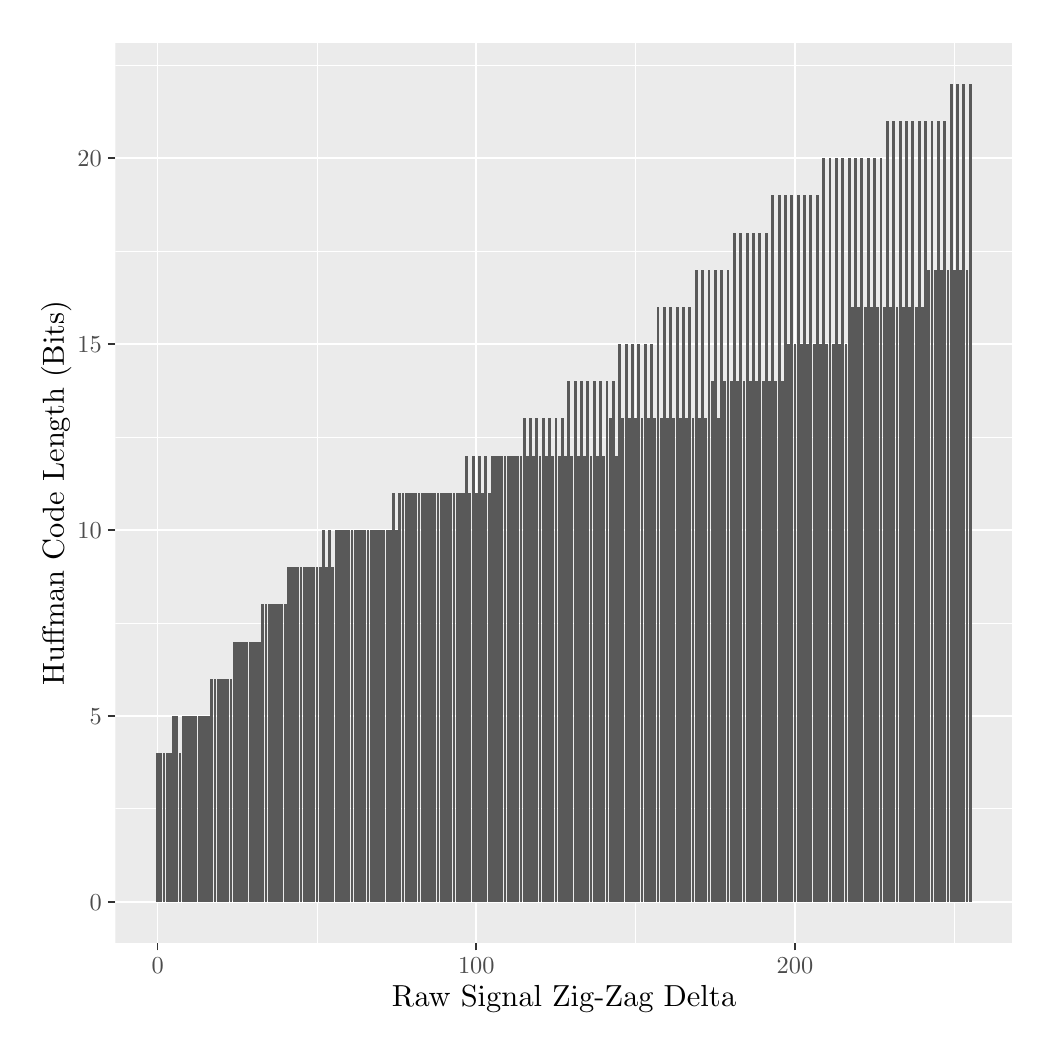
\begin{tikzpicture}[x=1pt,y=1pt]
\definecolor{fillColor}{RGB}{255,255,255}
\path[use as bounding box,fill=fillColor,fill opacity=0.00] (0,0) rectangle (361.35,361.35);
\begin{scope}
\path[clip] (  0.00,  0.00) rectangle (361.35,361.35);
\definecolor{drawColor}{RGB}{255,255,255}
\definecolor{fillColor}{RGB}{255,255,255}

\path[draw=drawColor,line width= 0.6pt,line join=round,line cap=round,fill=fillColor] (  0.00,  0.00) rectangle (361.35,361.35);
\end{scope}
\begin{scope}
\path[clip] ( 31.71, 30.69) rectangle (355.85,355.85);
\definecolor{fillColor}{gray}{0.92}

\path[fill=fillColor] ( 31.71, 30.69) rectangle (355.85,355.85);
\definecolor{drawColor}{RGB}{255,255,255}

\path[draw=drawColor,line width= 0.3pt,line join=round] ( 31.71, 79.06) --
	(355.85, 79.06);

\path[draw=drawColor,line width= 0.3pt,line join=round] ( 31.71,146.24) --
	(355.85,146.24);

\path[draw=drawColor,line width= 0.3pt,line join=round] ( 31.71,213.42) --
	(355.85,213.42);

\path[draw=drawColor,line width= 0.3pt,line join=round] ( 31.71,280.61) --
	(355.85,280.61);

\path[draw=drawColor,line width= 0.3pt,line join=round] ( 31.71,347.79) --
	(355.85,347.79);

\path[draw=drawColor,line width= 0.3pt,line join=round] (104.54, 30.69) --
	(104.54,355.85);

\path[draw=drawColor,line width= 0.3pt,line join=round] (219.69, 30.69) --
	(219.69,355.85);

\path[draw=drawColor,line width= 0.3pt,line join=round] (334.84, 30.69) --
	(334.84,355.85);

\path[draw=drawColor,line width= 0.6pt,line join=round] ( 31.71, 45.47) --
	(355.85, 45.47);

\path[draw=drawColor,line width= 0.6pt,line join=round] ( 31.71,112.65) --
	(355.85,112.65);

\path[draw=drawColor,line width= 0.6pt,line join=round] ( 31.71,179.83) --
	(355.85,179.83);

\path[draw=drawColor,line width= 0.6pt,line join=round] ( 31.71,247.01) --
	(355.85,247.01);

\path[draw=drawColor,line width= 0.6pt,line join=round] ( 31.71,314.20) --
	(355.85,314.20);

\path[draw=drawColor,line width= 0.6pt,line join=round] ( 46.96, 30.69) --
	( 46.96,355.85);

\path[draw=drawColor,line width= 0.6pt,line join=round] (162.11, 30.69) --
	(162.11,355.85);

\path[draw=drawColor,line width= 0.6pt,line join=round] (277.27, 30.69) --
	(277.27,355.85);
\definecolor{fillColor}{gray}{0.35}

\path[fill=fillColor] ( 46.45, 45.47) rectangle ( 47.48, 99.21);

\path[fill=fillColor] ( 47.60, 45.47) rectangle ( 48.63, 99.21);

\path[fill=fillColor] ( 48.75, 45.47) rectangle ( 49.79, 99.21);

\path[fill=fillColor] ( 49.90, 45.47) rectangle ( 50.94, 99.21);

\path[fill=fillColor] ( 51.05, 45.47) rectangle ( 52.09, 99.21);

\path[fill=fillColor] ( 52.20, 45.47) rectangle ( 53.24,112.65);

\path[fill=fillColor] ( 53.35, 45.47) rectangle ( 54.39,112.65);

\path[fill=fillColor] ( 54.51, 45.47) rectangle ( 55.54, 99.21);

\path[fill=fillColor] ( 55.66, 45.47) rectangle ( 56.69,112.65);

\path[fill=fillColor] ( 56.81, 45.47) rectangle ( 57.85,112.65);

\path[fill=fillColor] ( 57.96, 45.47) rectangle ( 59.00,112.65);

\path[fill=fillColor] ( 59.11, 45.47) rectangle ( 60.15,112.65);

\path[fill=fillColor] ( 60.26, 45.47) rectangle ( 61.30,112.65);

\path[fill=fillColor] ( 61.42, 45.47) rectangle ( 62.45,112.65);

\path[fill=fillColor] ( 62.57, 45.47) rectangle ( 63.60,112.65);

\path[fill=fillColor] ( 63.72, 45.47) rectangle ( 64.75,112.65);

\path[fill=fillColor] ( 64.87, 45.47) rectangle ( 65.91,112.65);

\path[fill=fillColor] ( 66.02, 45.47) rectangle ( 67.06,126.09);

\path[fill=fillColor] ( 67.17, 45.47) rectangle ( 68.21,126.09);

\path[fill=fillColor] ( 68.32, 45.47) rectangle ( 69.36,126.09);

\path[fill=fillColor] ( 69.48, 45.47) rectangle ( 70.51,126.09);

\path[fill=fillColor] ( 70.63, 45.47) rectangle ( 71.66,126.09);

\path[fill=fillColor] ( 71.78, 45.47) rectangle ( 72.82,126.09);

\path[fill=fillColor] ( 72.93, 45.47) rectangle ( 73.97,126.09);

\path[fill=fillColor] ( 74.08, 45.47) rectangle ( 75.12,139.52);

\path[fill=fillColor] ( 75.23, 45.47) rectangle ( 76.27,139.52);

\path[fill=fillColor] ( 76.38, 45.47) rectangle ( 77.42,139.52);

\path[fill=fillColor] ( 77.54, 45.47) rectangle ( 78.57,139.52);

\path[fill=fillColor] ( 78.69, 45.47) rectangle ( 79.72,139.52);

\path[fill=fillColor] ( 79.84, 45.47) rectangle ( 80.88,139.52);

\path[fill=fillColor] ( 80.99, 45.47) rectangle ( 82.03,139.52);

\path[fill=fillColor] ( 82.14, 45.47) rectangle ( 83.18,139.52);

\path[fill=fillColor] ( 83.29, 45.47) rectangle ( 84.33,139.52);

\path[fill=fillColor] ( 84.45, 45.47) rectangle ( 85.48,152.96);

\path[fill=fillColor] ( 85.60, 45.47) rectangle ( 86.63,152.96);

\path[fill=fillColor] ( 86.75, 45.47) rectangle ( 87.78,152.96);

\path[fill=fillColor] ( 87.90, 45.47) rectangle ( 88.94,152.96);

\path[fill=fillColor] ( 89.05, 45.47) rectangle ( 90.09,152.96);

\path[fill=fillColor] ( 90.20, 45.47) rectangle ( 91.24,152.96);

\path[fill=fillColor] ( 91.35, 45.47) rectangle ( 92.39,152.96);

\path[fill=fillColor] ( 92.51, 45.47) rectangle ( 93.54,152.96);

\path[fill=fillColor] ( 93.66, 45.47) rectangle ( 94.69,166.39);

\path[fill=fillColor] ( 94.81, 45.47) rectangle ( 95.85,166.39);

\path[fill=fillColor] ( 95.96, 45.47) rectangle ( 97.00,166.39);

\path[fill=fillColor] ( 97.11, 45.47) rectangle ( 98.15,166.39);

\path[fill=fillColor] ( 98.26, 45.47) rectangle ( 99.30,166.39);

\path[fill=fillColor] ( 99.42, 45.47) rectangle (100.45,166.39);

\path[fill=fillColor] (100.57, 45.47) rectangle (101.60,166.39);

\path[fill=fillColor] (101.72, 45.47) rectangle (102.75,166.39);

\path[fill=fillColor] (102.87, 45.47) rectangle (103.91,166.39);

\path[fill=fillColor] (104.02, 45.47) rectangle (105.06,166.39);

\path[fill=fillColor] (105.17, 45.47) rectangle (106.21,166.39);

\path[fill=fillColor] (106.32, 45.47) rectangle (107.36,179.83);

\path[fill=fillColor] (107.48, 45.47) rectangle (108.51,166.39);

\path[fill=fillColor] (108.63, 45.47) rectangle (109.66,179.83);

\path[fill=fillColor] (109.78, 45.47) rectangle (110.82,166.39);

\path[fill=fillColor] (110.93, 45.47) rectangle (111.97,179.83);

\path[fill=fillColor] (112.08, 45.47) rectangle (113.12,179.83);

\path[fill=fillColor] (113.23, 45.47) rectangle (114.27,179.83);

\path[fill=fillColor] (114.38, 45.47) rectangle (115.42,179.83);

\path[fill=fillColor] (115.54, 45.47) rectangle (116.57,179.83);

\path[fill=fillColor] (116.69, 45.47) rectangle (117.72,179.83);

\path[fill=fillColor] (117.84, 45.47) rectangle (118.88,179.83);

\path[fill=fillColor] (118.99, 45.47) rectangle (120.03,179.83);

\path[fill=fillColor] (120.14, 45.47) rectangle (121.18,179.83);

\path[fill=fillColor] (121.29, 45.47) rectangle (122.33,179.83);

\path[fill=fillColor] (122.45, 45.47) rectangle (123.48,179.83);

\path[fill=fillColor] (123.60, 45.47) rectangle (124.63,179.83);

\path[fill=fillColor] (124.75, 45.47) rectangle (125.78,179.83);

\path[fill=fillColor] (125.90, 45.47) rectangle (126.94,179.83);

\path[fill=fillColor] (127.05, 45.47) rectangle (128.09,179.83);

\path[fill=fillColor] (128.20, 45.47) rectangle (129.24,179.83);

\path[fill=fillColor] (129.35, 45.47) rectangle (130.39,179.83);

\path[fill=fillColor] (130.51, 45.47) rectangle (131.54,179.83);

\path[fill=fillColor] (131.66, 45.47) rectangle (132.69,193.27);

\path[fill=fillColor] (132.81, 45.47) rectangle (133.85,179.83);

\path[fill=fillColor] (133.96, 45.47) rectangle (135.00,193.27);

\path[fill=fillColor] (135.11, 45.47) rectangle (136.15,193.27);

\path[fill=fillColor] (136.26, 45.47) rectangle (137.30,193.27);

\path[fill=fillColor] (137.41, 45.47) rectangle (138.45,193.27);

\path[fill=fillColor] (138.57, 45.47) rectangle (139.60,193.27);

\path[fill=fillColor] (139.72, 45.47) rectangle (140.75,193.27);

\path[fill=fillColor] (140.87, 45.47) rectangle (141.91,193.27);

\path[fill=fillColor] (142.02, 45.47) rectangle (143.06,193.27);

\path[fill=fillColor] (143.17, 45.47) rectangle (144.21,193.27);

\path[fill=fillColor] (144.32, 45.47) rectangle (145.36,193.27);

\path[fill=fillColor] (145.48, 45.47) rectangle (146.51,193.27);

\path[fill=fillColor] (146.63, 45.47) rectangle (147.66,193.27);

\path[fill=fillColor] (147.78, 45.47) rectangle (148.81,193.27);

\path[fill=fillColor] (148.93, 45.47) rectangle (149.97,193.27);

\path[fill=fillColor] (150.08, 45.47) rectangle (151.12,193.27);

\path[fill=fillColor] (151.23, 45.47) rectangle (152.27,193.27);

\path[fill=fillColor] (152.38, 45.47) rectangle (153.42,193.27);

\path[fill=fillColor] (153.54, 45.47) rectangle (154.57,193.27);

\path[fill=fillColor] (154.69, 45.47) rectangle (155.72,193.27);

\path[fill=fillColor] (155.84, 45.47) rectangle (156.88,193.27);

\path[fill=fillColor] (156.99, 45.47) rectangle (158.03,193.27);

\path[fill=fillColor] (158.14, 45.47) rectangle (159.18,206.70);

\path[fill=fillColor] (159.29, 45.47) rectangle (160.33,193.27);

\path[fill=fillColor] (160.44, 45.47) rectangle (161.48,206.70);

\path[fill=fillColor] (161.60, 45.47) rectangle (162.63,193.27);

\path[fill=fillColor] (162.75, 45.47) rectangle (163.78,206.70);

\path[fill=fillColor] (163.90, 45.47) rectangle (164.94,193.27);

\path[fill=fillColor] (165.05, 45.47) rectangle (166.09,206.70);

\path[fill=fillColor] (166.20, 45.47) rectangle (167.24,193.27);

\path[fill=fillColor] (167.35, 45.47) rectangle (168.39,206.70);

\path[fill=fillColor] (168.51, 45.47) rectangle (169.54,206.70);

\path[fill=fillColor] (169.66, 45.47) rectangle (170.69,206.70);

\path[fill=fillColor] (170.81, 45.47) rectangle (171.84,206.70);

\path[fill=fillColor] (171.96, 45.47) rectangle (173.00,206.70);

\path[fill=fillColor] (173.11, 45.47) rectangle (174.15,206.70);

\path[fill=fillColor] (174.26, 45.47) rectangle (175.30,206.70);

\path[fill=fillColor] (175.41, 45.47) rectangle (176.45,206.70);

\path[fill=fillColor] (176.57, 45.47) rectangle (177.60,206.70);

\path[fill=fillColor] (177.72, 45.47) rectangle (178.75,206.70);

\path[fill=fillColor] (178.87, 45.47) rectangle (179.91,220.14);

\path[fill=fillColor] (180.02, 45.47) rectangle (181.06,206.70);

\path[fill=fillColor] (181.17, 45.47) rectangle (182.21,220.14);

\path[fill=fillColor] (182.32, 45.47) rectangle (183.36,206.70);

\path[fill=fillColor] (183.48, 45.47) rectangle (184.51,220.14);

\path[fill=fillColor] (184.63, 45.47) rectangle (185.66,206.70);

\path[fill=fillColor] (185.78, 45.47) rectangle (186.81,220.14);

\path[fill=fillColor] (186.93, 45.47) rectangle (187.97,206.70);

\path[fill=fillColor] (188.08, 45.47) rectangle (189.12,220.14);

\path[fill=fillColor] (189.23, 45.47) rectangle (190.27,206.70);

\path[fill=fillColor] (190.38, 45.47) rectangle (191.42,220.14);

\path[fill=fillColor] (191.54, 45.47) rectangle (192.57,206.70);

\path[fill=fillColor] (192.69, 45.47) rectangle (193.72,220.14);

\path[fill=fillColor] (193.84, 45.47) rectangle (194.88,206.70);

\path[fill=fillColor] (194.99, 45.47) rectangle (196.03,233.58);

\path[fill=fillColor] (196.14, 45.47) rectangle (197.18,206.70);

\path[fill=fillColor] (197.29, 45.47) rectangle (198.33,233.58);

\path[fill=fillColor] (198.44, 45.47) rectangle (199.48,206.70);

\path[fill=fillColor] (199.60, 45.47) rectangle (200.63,233.58);

\path[fill=fillColor] (200.75, 45.47) rectangle (201.78,206.70);

\path[fill=fillColor] (201.90, 45.47) rectangle (202.94,233.58);

\path[fill=fillColor] (203.05, 45.47) rectangle (204.09,206.70);

\path[fill=fillColor] (204.20, 45.47) rectangle (205.24,233.58);

\path[fill=fillColor] (205.35, 45.47) rectangle (206.39,206.70);

\path[fill=fillColor] (206.51, 45.47) rectangle (207.54,233.58);

\path[fill=fillColor] (207.66, 45.47) rectangle (208.69,206.70);

\path[fill=fillColor] (208.81, 45.47) rectangle (209.84,233.58);

\path[fill=fillColor] (209.96, 45.47) rectangle (211.00,220.14);

\path[fill=fillColor] (211.11, 45.47) rectangle (212.15,233.58);

\path[fill=fillColor] (212.26, 45.47) rectangle (213.30,206.70);

\path[fill=fillColor] (213.41, 45.47) rectangle (214.45,247.01);

\path[fill=fillColor] (214.57, 45.47) rectangle (215.60,220.14);

\path[fill=fillColor] (215.72, 45.47) rectangle (216.75,247.01);

\path[fill=fillColor] (216.87, 45.47) rectangle (217.91,220.14);

\path[fill=fillColor] (218.02, 45.47) rectangle (219.06,247.01);

\path[fill=fillColor] (219.17, 45.47) rectangle (220.21,220.14);

\path[fill=fillColor] (220.32, 45.47) rectangle (221.36,247.01);

\path[fill=fillColor] (221.47, 45.47) rectangle (222.51,220.14);

\path[fill=fillColor] (222.63, 45.47) rectangle (223.66,247.01);

\path[fill=fillColor] (223.78, 45.47) rectangle (224.81,220.14);

\path[fill=fillColor] (224.93, 45.47) rectangle (225.97,247.01);

\path[fill=fillColor] (226.08, 45.47) rectangle (227.12,220.14);

\path[fill=fillColor] (227.23, 45.47) rectangle (228.27,260.45);

\path[fill=fillColor] (228.38, 45.47) rectangle (229.42,220.14);

\path[fill=fillColor] (229.54, 45.47) rectangle (230.57,260.45);

\path[fill=fillColor] (230.69, 45.47) rectangle (231.72,220.14);

\path[fill=fillColor] (231.84, 45.47) rectangle (232.87,260.45);

\path[fill=fillColor] (232.99, 45.47) rectangle (234.03,220.14);

\path[fill=fillColor] (234.14, 45.47) rectangle (235.18,260.45);

\path[fill=fillColor] (235.29, 45.47) rectangle (236.33,220.14);

\path[fill=fillColor] (236.44, 45.47) rectangle (237.48,260.45);

\path[fill=fillColor] (237.60, 45.47) rectangle (238.63,220.14);

\path[fill=fillColor] (238.75, 45.47) rectangle (239.78,260.45);

\path[fill=fillColor] (239.90, 45.47) rectangle (240.94,220.14);

\path[fill=fillColor] (241.05, 45.47) rectangle (242.09,273.89);

\path[fill=fillColor] (242.20, 45.47) rectangle (243.24,220.14);

\path[fill=fillColor] (243.35, 45.47) rectangle (244.39,273.89);

\path[fill=fillColor] (244.51, 45.47) rectangle (245.54,220.14);

\path[fill=fillColor] (245.66, 45.47) rectangle (246.69,273.89);

\path[fill=fillColor] (246.81, 45.47) rectangle (247.84,233.58);

\path[fill=fillColor] (247.96, 45.47) rectangle (249.00,273.89);

\path[fill=fillColor] (249.11, 45.47) rectangle (250.15,220.14);

\path[fill=fillColor] (250.26, 45.47) rectangle (251.30,273.89);

\path[fill=fillColor] (251.41, 45.47) rectangle (252.45,233.58);

\path[fill=fillColor] (252.57, 45.47) rectangle (253.60,273.89);

\path[fill=fillColor] (253.72, 45.47) rectangle (254.75,233.58);

\path[fill=fillColor] (254.87, 45.47) rectangle (255.90,287.32);

\path[fill=fillColor] (256.02, 45.47) rectangle (257.06,233.58);

\path[fill=fillColor] (257.17, 45.47) rectangle (258.21,287.32);

\path[fill=fillColor] (258.32, 45.47) rectangle (259.36,233.58);

\path[fill=fillColor] (259.47, 45.47) rectangle (260.51,287.32);

\path[fill=fillColor] (260.63, 45.47) rectangle (261.66,233.58);

\path[fill=fillColor] (261.78, 45.47) rectangle (262.81,287.32);

\path[fill=fillColor] (262.93, 45.47) rectangle (263.97,233.58);

\path[fill=fillColor] (264.08, 45.47) rectangle (265.12,287.32);

\path[fill=fillColor] (265.23, 45.47) rectangle (266.27,233.58);

\path[fill=fillColor] (266.38, 45.47) rectangle (267.42,287.32);

\path[fill=fillColor] (267.54, 45.47) rectangle (268.57,233.58);

\path[fill=fillColor] (268.69, 45.47) rectangle (269.72,300.76);

\path[fill=fillColor] (269.84, 45.47) rectangle (270.87,233.58);

\path[fill=fillColor] (270.99, 45.47) rectangle (272.03,300.76);

\path[fill=fillColor] (272.14, 45.47) rectangle (273.18,233.58);

\path[fill=fillColor] (273.29, 45.47) rectangle (274.33,300.76);

\path[fill=fillColor] (274.44, 45.47) rectangle (275.48,247.01);

\path[fill=fillColor] (275.60, 45.47) rectangle (276.63,300.76);

\path[fill=fillColor] (276.75, 45.47) rectangle (277.78,247.01);

\path[fill=fillColor] (277.90, 45.47) rectangle (278.94,300.76);

\path[fill=fillColor] (279.05, 45.47) rectangle (280.09,247.01);

\path[fill=fillColor] (280.20, 45.47) rectangle (281.24,300.76);

\path[fill=fillColor] (281.35, 45.47) rectangle (282.39,247.01);

\path[fill=fillColor] (282.50, 45.47) rectangle (283.54,300.76);

\path[fill=fillColor] (283.66, 45.47) rectangle (284.69,247.01);

\path[fill=fillColor] (284.81, 45.47) rectangle (285.84,300.76);

\path[fill=fillColor] (285.96, 45.47) rectangle (287.00,247.01);

\path[fill=fillColor] (287.11, 45.47) rectangle (288.15,314.20);

\path[fill=fillColor] (288.26, 45.47) rectangle (289.30,247.01);

\path[fill=fillColor] (289.41, 45.47) rectangle (290.45,314.20);

\path[fill=fillColor] (290.57, 45.47) rectangle (291.60,247.01);

\path[fill=fillColor] (291.72, 45.47) rectangle (292.75,314.20);

\path[fill=fillColor] (292.87, 45.47) rectangle (293.90,247.01);

\path[fill=fillColor] (294.02, 45.47) rectangle (295.06,314.20);

\path[fill=fillColor] (295.17, 45.47) rectangle (296.21,247.01);

\path[fill=fillColor] (296.32, 45.47) rectangle (297.36,314.20);

\path[fill=fillColor] (297.47, 45.47) rectangle (298.51,260.45);

\path[fill=fillColor] (298.63, 45.47) rectangle (299.66,314.20);

\path[fill=fillColor] (299.78, 45.47) rectangle (300.81,260.45);

\path[fill=fillColor] (300.93, 45.47) rectangle (301.97,314.20);

\path[fill=fillColor] (302.08, 45.47) rectangle (303.12,260.45);

\path[fill=fillColor] (303.23, 45.47) rectangle (304.27,314.20);

\path[fill=fillColor] (304.38, 45.47) rectangle (305.42,260.45);

\path[fill=fillColor] (305.53, 45.47) rectangle (306.57,314.20);

\path[fill=fillColor] (306.69, 45.47) rectangle (307.72,260.45);

\path[fill=fillColor] (307.84, 45.47) rectangle (308.87,314.20);

\path[fill=fillColor] (308.99, 45.47) rectangle (310.03,260.45);

\path[fill=fillColor] (310.14, 45.47) rectangle (311.18,327.63);

\path[fill=fillColor] (311.29, 45.47) rectangle (312.33,260.45);

\path[fill=fillColor] (312.44, 45.47) rectangle (313.48,327.63);

\path[fill=fillColor] (313.60, 45.47) rectangle (314.63,260.45);

\path[fill=fillColor] (314.75, 45.47) rectangle (315.78,327.63);

\path[fill=fillColor] (315.90, 45.47) rectangle (316.93,260.45);

\path[fill=fillColor] (317.05, 45.47) rectangle (318.09,327.63);

\path[fill=fillColor] (318.20, 45.47) rectangle (319.24,260.45);

\path[fill=fillColor] (319.35, 45.47) rectangle (320.39,327.63);

\path[fill=fillColor] (320.50, 45.47) rectangle (321.54,260.45);

\path[fill=fillColor] (321.66, 45.47) rectangle (322.69,327.63);

\path[fill=fillColor] (322.81, 45.47) rectangle (323.84,260.45);

\path[fill=fillColor] (323.96, 45.47) rectangle (325.00,327.63);

\path[fill=fillColor] (325.11, 45.47) rectangle (326.15,273.89);

\path[fill=fillColor] (326.26, 45.47) rectangle (327.30,327.63);

\path[fill=fillColor] (327.41, 45.47) rectangle (328.45,273.89);

\path[fill=fillColor] (328.57, 45.47) rectangle (329.60,327.63);

\path[fill=fillColor] (329.72, 45.47) rectangle (330.75,273.89);

\path[fill=fillColor] (330.87, 45.47) rectangle (331.90,327.63);

\path[fill=fillColor] (332.02, 45.47) rectangle (333.06,273.89);

\path[fill=fillColor] (333.17, 45.47) rectangle (334.21,341.07);

\path[fill=fillColor] (334.32, 45.47) rectangle (335.36,273.89);

\path[fill=fillColor] (335.47, 45.47) rectangle (336.51,341.07);

\path[fill=fillColor] (336.63, 45.47) rectangle (337.66,273.89);

\path[fill=fillColor] (337.78, 45.47) rectangle (338.81,341.07);

\path[fill=fillColor] (338.93, 45.47) rectangle (339.96,273.89);

\path[fill=fillColor] (340.08, 45.47) rectangle (341.12,341.07);
\end{scope}
\begin{scope}
\path[clip] (  0.00,  0.00) rectangle (361.35,361.35);
\definecolor{drawColor}{gray}{0.30}

\node[text=drawColor,anchor=base east,inner sep=0pt, outer sep=0pt, scale=  0.88] at ( 26.76, 42.44) {0};

\node[text=drawColor,anchor=base east,inner sep=0pt, outer sep=0pt, scale=  0.88] at ( 26.76,109.62) {5};

\node[text=drawColor,anchor=base east,inner sep=0pt, outer sep=0pt, scale=  0.88] at ( 26.76,176.80) {10};

\node[text=drawColor,anchor=base east,inner sep=0pt, outer sep=0pt, scale=  0.88] at ( 26.76,243.98) {15};

\node[text=drawColor,anchor=base east,inner sep=0pt, outer sep=0pt, scale=  0.88] at ( 26.76,311.17) {20};
\end{scope}
\begin{scope}
\path[clip] (  0.00,  0.00) rectangle (361.35,361.35);
\definecolor{drawColor}{gray}{0.20}

\path[draw=drawColor,line width= 0.6pt,line join=round] ( 28.96, 45.47) --
	( 31.71, 45.47);

\path[draw=drawColor,line width= 0.6pt,line join=round] ( 28.96,112.65) --
	( 31.71,112.65);

\path[draw=drawColor,line width= 0.6pt,line join=round] ( 28.96,179.83) --
	( 31.71,179.83);

\path[draw=drawColor,line width= 0.6pt,line join=round] ( 28.96,247.01) --
	( 31.71,247.01);

\path[draw=drawColor,line width= 0.6pt,line join=round] ( 28.96,314.20) --
	( 31.71,314.20);
\end{scope}
\begin{scope}
\path[clip] (  0.00,  0.00) rectangle (361.35,361.35);
\definecolor{drawColor}{gray}{0.20}

\path[draw=drawColor,line width= 0.6pt,line join=round] ( 46.96, 27.94) --
	( 46.96, 30.69);

\path[draw=drawColor,line width= 0.6pt,line join=round] (162.11, 27.94) --
	(162.11, 30.69);

\path[draw=drawColor,line width= 0.6pt,line join=round] (277.27, 27.94) --
	(277.27, 30.69);
\end{scope}
\begin{scope}
\path[clip] (  0.00,  0.00) rectangle (361.35,361.35);
\definecolor{drawColor}{gray}{0.30}

\node[text=drawColor,anchor=base,inner sep=0pt, outer sep=0pt, scale=  0.88] at ( 46.96, 19.68) {0};

\node[text=drawColor,anchor=base,inner sep=0pt, outer sep=0pt, scale=  0.88] at (162.11, 19.68) {100};

\node[text=drawColor,anchor=base,inner sep=0pt, outer sep=0pt, scale=  0.88] at (277.27, 19.68) {200};
\end{scope}
\begin{scope}
\path[clip] (  0.00,  0.00) rectangle (361.35,361.35);
\definecolor{drawColor}{RGB}{0,0,0}

\node[text=drawColor,anchor=base,inner sep=0pt, outer sep=0pt, scale=  1.10] at (193.78,  7.64) {Raw Signal Zig-Zag Delta};
\end{scope}
\begin{scope}
\path[clip] (  0.00,  0.00) rectangle (361.35,361.35);
\definecolor{drawColor}{RGB}{0,0,0}

\node[text=drawColor,rotate= 90.00,anchor=base,inner sep=0pt, outer sep=0pt, scale=  1.10] at ( 13.08,193.27) {Huffman Code Length (Bits)};
\end{scope}
\end{tikzpicture}

	\caption[The Huffman code length of each one-byte zig-zag delta from the shared Huffman table.]{\label{fig:shuff-len}The Huffman code length of each one-byte zig-zag delta from the shared Huffman table, generated using the frequency distribution of the whole data set.}
\end{figure}


\subsection{Range Coding}

Now consider encoding the one-byte data using range coding rather than Huffman
coding. Recall that range coding encodes all of the data into one number given
each symbol's probability of occurrence.  An appropriate initial range of
numbers is chosen. Then, for each symbol in the data stream the current range is
narrowed down based on the current symbol's probability of occurrence. A
representative number from the final range is then chosen as the output.

The probability distribution can be predetermined, calculated by an initial pass
or predicted adaptively. Most available implementations use models
for predicting the probability distribution of the next symbol. These typically
consist of models such as order-0, order-1, order-2 and context mixing which combines
two such algorithms to yield higher accuracy predictions. Secondary symbol
estimation (SSE) is a prediction postprocessing approach which uses the combined
prediction of context mixing and a small context to generate a refined
prediction. The range coding algorithm which applies order-0 and order-1 context
mixing with SSE we'll abbreviate to \textit{rccm01sse}.

The order-$n$ model gives the probability distribution of the next symbol given
the previous $n$ symbols (context). It is updated at each step to increase the
revealed symbol's probability when the same context appears again. For example,
the order-0 model stores the probability distribution of the data up to the
current symbol.

% http://mattmahoney.net/dc/dce.html


\section{Exploiting the Signal}

As discussed in Section
\ref{sec:data:char},
there are several predictable characteristics among reads which can be exploited
to gain more compression.

\subsection{The Stall}

To begin with, recall that the stall is the section of a read which occurs at
the beginning between the surge and pre-adapter surge. It is thought to occur
due to the motor protein `stalling' before it begins to unwind the molecule.
% See Figure \ref{}
It consists of hundreds to thousands of data points which oscillate with little
variation around the read's median. The stall is a highly likely occurrence in
any read but its length and variance changes from read to read.

Only 6 reads in the data set do not have a stall. The minimum stall length is 34
with a maximum of \num{37128} and mean of 1140.33. But the standard deviation is
quite large at 1214.78. See Table \ref{tab:stall-n}. The standard deviation of
raw signal values in a stall is 5.72 compared to 35.07 for the whole data set.

\begin{table}
    \caption{\label{tab:stall-n} Summary statistics of the data's stall lengths.}
    \begin{tabular}{|l|l|}
        \hline
Min & 34\\
	    Q1 & 314\\

Q2 & 771\\
	    Q3 & 1156\\
Max & 37128\\
\hline
Mean & 1140.33\\
	    Mode & 39\\
Sample SD & 1214.781\\
	\hline
    \end{tabular}
\end{table}


We can take advantage of this section by compressing it separately if it is
large enough using the frame of reference algorithm followed by some encoding.
Since it oscillates with little variance around the read's median, the distance
from each point to the stall's minimum is smaller than in most other sections.
Instead of computing the zig-zag deltas we subtract the minimum point in the
stall from all other stall points then apply an entropy encoder such as
rc-vbe21.

The encoding stores the stall's starting index (2 bytes), length (2 bytes),
compressed size (2 bytes) and compressed data (variable bytes) followed by the
non-stall's compressed size (4 bytes) and compressed data (variable bytes). This
method is more space-advantageous if
\[ C_{stall}(r) = C_{specific}(r_s) + C_{generic}(r\setminus r_s) + 10 < C_{generic}(r) \]
where $r\in\Omega$ is a read from the space of possible reads and $r_s$ is the
read's stall section. That is, this method is advantageous if its total
compressed size, consisting of the compressed stall, the compressed non-stall
and 10 bytes of metadata, is less than the usual encoding.

% TODO put diagram of encoding

The encoding could actually dynamically make the above comparison to decide
whether the stall is worth encoding or not. Then it could store an extra bit (or
byte for convenience) to mark whether the stall or generic algorithm is being
used. Let's name this algorithm the \textit{dynamic stall} encoding or
\textit{dstall} for short. However, this extra bit or byte is a waste of space
if the large majority of reads benefit from a specific stall encoding and
vice-versa for generic stall encoding.

Consider our specific algorithm to be the FOR encoding followed by the compact
variable byte exceptions encoding (vbbe21) and range coding (or
\textit{rc-vbbe21-for} for short). Due to its compression performance so far,
let's consider the generic algorithm to be rc-vbbe21-zd where \textit{zd} stands
for zig-zag delta. Let's compare their performance on different length stalls.

\subsection{Separating the Jumps and Flats}

The large majority of the data consists of DNA sections so any gains in
compression discovered by understanding this type of section should
result in the largest compression gains overall.

The problem is that there are a lot of apparent irregularities in the DNA
sections as is expected with information saturated sensor data. Furthermore, the
zig-zag delta transformation is quite fast and already has a readily
compressible distribution making it difficult to outperform. However, one
observation we could take advantage of is the fact that the signal tends to
suddenly move up or down between `flat' sections which oscillate around some
level. See Figure \ref{fig:dna300-section}. Another observation is that the
signal tends to move around the same median -- that is, if it moves up it is
more likely to move down soon. This is obvious if we refer back to the
distribution of deltas (Figure \ref{fig:delta-hist}) where it is clearly
symmetric except at the tails.

\begin{figure}
\centering
% Created by tikzDevice version 0.12.3.1 on 2022-10-19 12:01:19
% !TEX encoding = UTF-8 Unicode
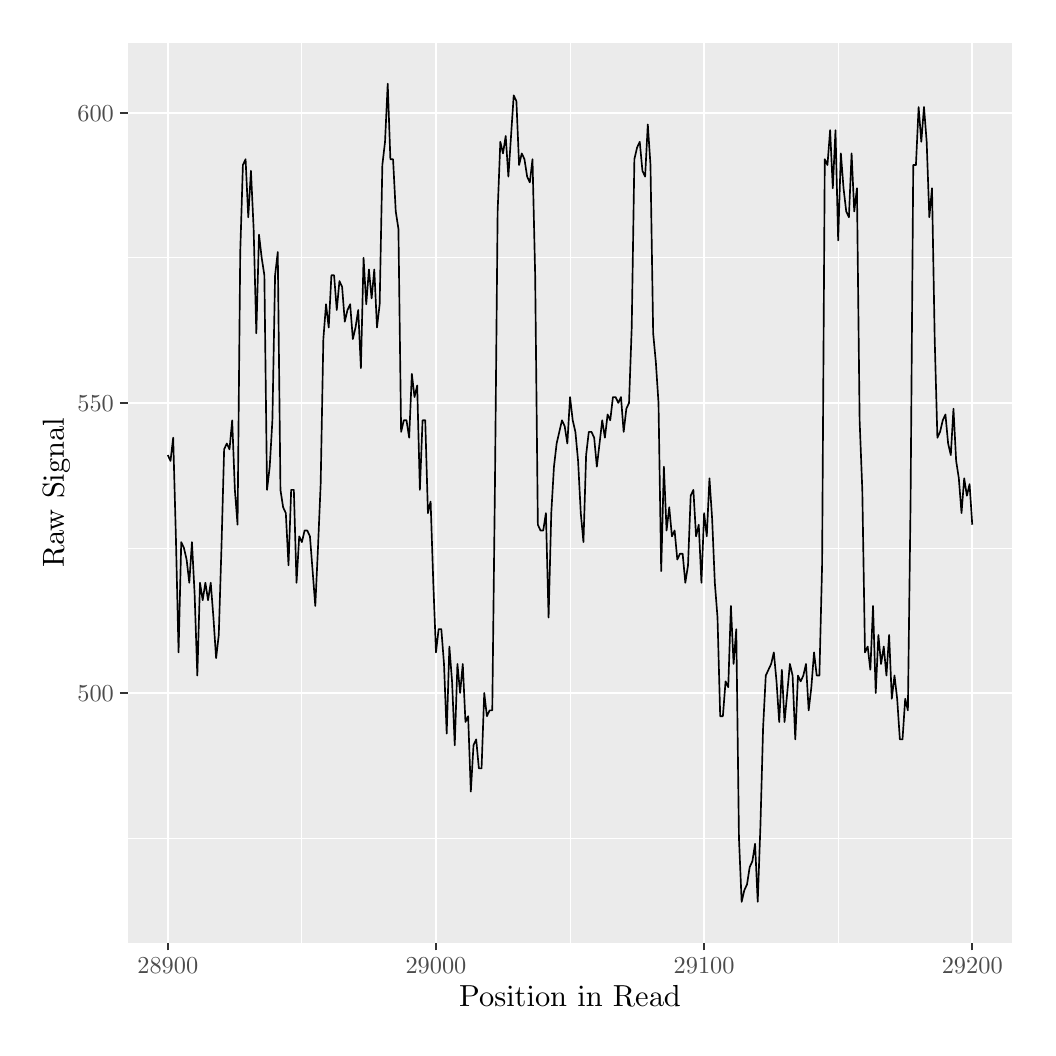
\begin{tikzpicture}[x=1pt,y=1pt]
\definecolor{fillColor}{RGB}{255,255,255}
\path[use as bounding box,fill=fillColor,fill opacity=0.00] (0,0) rectangle (361.35,361.35);
\begin{scope}
\path[clip] (  0.00,  0.00) rectangle (361.35,361.35);
\definecolor{drawColor}{RGB}{255,255,255}
\definecolor{fillColor}{RGB}{255,255,255}

\path[draw=drawColor,line width= 0.6pt,line join=round,line cap=round,fill=fillColor] (  0.00,  0.00) rectangle (361.35,361.35);
\end{scope}
\begin{scope}
\path[clip] ( 36.11, 30.69) rectangle (355.85,355.85);
\definecolor{fillColor}{gray}{0.92}

\path[fill=fillColor] ( 36.11, 30.69) rectangle (355.85,355.85);
\definecolor{drawColor}{RGB}{255,255,255}

\path[draw=drawColor,line width= 0.3pt,line join=round] ( 36.11, 68.53) --
	(355.85, 68.53);

\path[draw=drawColor,line width= 0.3pt,line join=round] ( 36.11,173.35) --
	(355.85,173.35);

\path[draw=drawColor,line width= 0.3pt,line join=round] ( 36.11,278.18) --
	(355.85,278.18);

\path[draw=drawColor,line width= 0.3pt,line join=round] ( 99.09, 30.69) --
	( 99.09,355.85);

\path[draw=drawColor,line width= 0.3pt,line join=round] (195.98, 30.69) --
	(195.98,355.85);

\path[draw=drawColor,line width= 0.3pt,line join=round] (292.87, 30.69) --
	(292.87,355.85);

\path[draw=drawColor,line width= 0.6pt,line join=round] ( 36.11,120.94) --
	(355.85,120.94);

\path[draw=drawColor,line width= 0.6pt,line join=round] ( 36.11,225.76) --
	(355.85,225.76);

\path[draw=drawColor,line width= 0.6pt,line join=round] ( 36.11,330.59) --
	(355.85,330.59);

\path[draw=drawColor,line width= 0.6pt,line join=round] ( 50.64, 30.69) --
	( 50.64,355.85);

\path[draw=drawColor,line width= 0.6pt,line join=round] (147.54, 30.69) --
	(147.54,355.85);

\path[draw=drawColor,line width= 0.6pt,line join=round] (244.43, 30.69) --
	(244.43,355.85);

\path[draw=drawColor,line width= 0.6pt,line join=round] (341.32, 30.69) --
	(341.32,355.85);
\definecolor{drawColor}{RGB}{0,0,0}

\path[draw=drawColor,line width= 0.6pt,line join=round] ( 50.64,206.90) --
	( 51.61,204.80) --
	( 52.58,213.18) --
	( 53.55,177.54) --
	( 54.52,135.61) --
	( 55.49,175.45) --
	( 56.46,173.35) --
	( 57.43,169.16) --
	( 58.40,160.77) --
	( 59.36,175.45) --
	( 60.33,156.58) --
	( 61.30,127.23) --
	( 62.27,160.77) --
	( 63.24,154.48) --
	( 64.21,160.77) --
	( 65.18,154.48) --
	( 66.15,160.77) --
	( 67.12,148.19) --
	( 68.09,133.52) --
	( 69.05,141.90) --
	( 70.02,173.35) --
	( 70.99,208.99) --
	( 71.96,211.09) --
	( 72.93,208.99) --
	( 73.90,219.47) --
	( 74.87,194.32) --
	( 75.84,181.74) --
	( 76.81,280.27) --
	( 77.77,311.72) --
	( 78.74,313.82) --
	( 79.71,292.85) --
	( 80.68,309.62) --
	( 81.65,288.66) --
	( 82.62,250.92) --
	( 83.59,286.56) --
	( 84.56,278.18) --
	( 85.53,271.89) --
	( 86.49,194.32) --
	( 87.46,202.70) --
	( 88.43,219.47) --
	( 89.40,271.89) --
	( 90.37,280.27) --
	( 91.34,194.32) --
	( 92.31,188.03) --
	( 93.28,185.93) --
	( 94.25,167.06) --
	( 95.21,194.32) --
	( 96.18,194.32) --
	( 97.15,160.77) --
	( 98.12,177.54) --
	( 99.09,175.45) --
	(100.06,179.64) --
	(101.03,179.64) --
	(102.00,177.54) --
	(102.97,164.97) --
	(103.93,152.39) --
	(104.90,173.35) --
	(105.87,196.41) --
	(106.84,248.82) --
	(107.81,261.40) --
	(108.78,253.02) --
	(109.75,271.89) --
	(110.72,271.89) --
	(111.69,259.31) --
	(112.65,269.79) --
	(113.62,267.69) --
	(114.59,255.11) --
	(115.56,259.31) --
	(116.53,261.40) --
	(117.50,248.82) --
	(118.47,253.02) --
	(119.44,259.31) --
	(120.41,238.34) --
	(121.37,278.18) --
	(122.34,261.40) --
	(123.31,273.98) --
	(124.28,263.50) --
	(125.25,273.98) --
	(126.22,253.02) --
	(127.19,261.40) --
	(128.16,311.72) --
	(129.13,320.11) --
	(130.10,341.07) --
	(131.06,313.82) --
	(132.03,313.82) --
	(133.00,294.95) --
	(133.97,288.66) --
	(134.94,215.28) --
	(135.91,219.47) --
	(136.88,219.47) --
	(137.85,213.18) --
	(138.82,236.25) --
	(139.78,227.86) --
	(140.75,232.05) --
	(141.72,194.32) --
	(142.69,219.47) --
	(143.66,219.47) --
	(144.63,185.93) --
	(145.60,190.12) --
	(146.57,160.77) --
	(147.54,135.61) --
	(148.50,144.00) --
	(149.47,144.00) --
	(150.44,131.42) --
	(151.41,106.26) --
	(152.38,137.71) --
	(153.35,125.13) --
	(154.32,102.07) --
	(155.29,131.42) --
	(156.26,120.94) --
	(157.22,131.42) --
	(158.19,110.46) --
	(159.16,112.55) --
	(160.13, 85.30) --
	(161.10,102.07) --
	(162.07,104.17) --
	(163.04, 93.69) --
	(164.01, 93.69) --
	(164.98,120.94) --
	(165.94,112.55) --
	(166.91,114.65) --
	(167.88,114.65) --
	(168.85,196.41) --
	(169.82,294.95) --
	(170.79,320.11) --
	(171.76,315.91) --
	(172.73,322.20) --
	(173.70,307.53) --
	(174.66,322.20) --
	(175.63,336.88) --
	(176.60,334.78) --
	(177.57,311.72) --
	(178.54,315.91) --
	(179.51,313.82) --
	(180.48,307.53) --
	(181.45,305.43) --
	(182.42,313.82) --
	(183.38,271.89) --
	(184.35,181.74) --
	(185.32,179.64) --
	(186.29,179.64) --
	(187.26,185.93) --
	(188.23,148.19) --
	(189.20,185.93) --
	(190.17,202.70) --
	(191.14,211.09) --
	(192.10,215.28) --
	(193.07,219.47) --
	(194.04,217.38) --
	(195.01,211.09) --
	(195.98,227.86) --
	(196.95,219.47) --
	(197.92,215.28) --
	(198.89,204.80) --
	(199.86,185.93) --
	(200.83,175.45) --
	(201.79,206.90) --
	(202.76,215.28) --
	(203.73,215.28) --
	(204.70,213.18) --
	(205.67,202.70) --
	(206.64,211.09) --
	(207.61,219.47) --
	(208.58,213.18) --
	(209.55,221.57) --
	(210.51,219.47) --
	(211.48,227.86) --
	(212.45,227.86) --
	(213.42,225.76) --
	(214.39,227.86) --
	(215.36,215.28) --
	(216.33,223.67) --
	(217.30,225.76) --
	(218.27,253.02) --
	(219.23,313.82) --
	(220.20,318.01) --
	(221.17,320.11) --
	(222.14,309.62) --
	(223.11,307.53) --
	(224.08,326.39) --
	(225.05,311.72) --
	(226.02,250.92) --
	(226.99,240.44) --
	(227.95,225.76) --
	(228.92,164.97) --
	(229.89,202.70) --
	(230.86,179.64) --
	(231.83,188.03) --
	(232.80,177.54) --
	(233.77,179.64) --
	(234.74,169.16) --
	(235.71,171.25) --
	(236.67,171.25) --
	(237.64,160.77) --
	(238.61,167.06) --
	(239.58,192.22) --
	(240.55,194.32) --
	(241.52,177.54) --
	(242.49,181.74) --
	(243.46,160.77) --
	(244.43,185.93) --
	(245.39,177.54) --
	(246.36,198.51) --
	(247.33,183.83) --
	(248.30,160.77) --
	(249.27,148.19) --
	(250.24,112.55) --
	(251.21,112.55) --
	(252.18,125.13) --
	(253.15,123.04) --
	(254.11,152.39) --
	(255.08,131.42) --
	(256.05,144.00) --
	(257.02, 68.53) --
	(257.99, 45.47) --
	(258.96, 49.66) --
	(259.93, 51.76) --
	(260.90, 58.04) --
	(261.87, 60.14) --
	(262.84, 66.43) --
	(263.80, 45.47) --
	(264.77, 72.72) --
	(265.74,108.36) --
	(266.71,127.23) --
	(267.68,129.33) --
	(268.65,131.42) --
	(269.62,135.61) --
	(270.59,125.13) --
	(271.56,110.46) --
	(272.52,129.33) --
	(273.49,110.46) --
	(274.46,120.94) --
	(275.43,131.42) --
	(276.40,127.23) --
	(277.37,104.17) --
	(278.34,127.23) --
	(279.31,125.13) --
	(280.28,127.23) --
	(281.24,131.42) --
	(282.21,114.65) --
	(283.18,123.04) --
	(284.15,135.61) --
	(285.12,127.23) --
	(286.09,127.23) --
	(287.06,167.06) --
	(288.03,313.82) --
	(289.00,311.72) --
	(289.96,324.30) --
	(290.93,303.33) --
	(291.90,324.30) --
	(292.87,284.46) --
	(293.84,315.91) --
	(294.81,303.33) --
	(295.78,294.95) --
	(296.75,292.85) --
	(297.72,315.91) --
	(298.68,294.95) --
	(299.65,303.33) --
	(300.62,219.47) --
	(301.59,194.32) --
	(302.56,135.61) --
	(303.53,137.71) --
	(304.50,129.33) --
	(305.47,152.39) --
	(306.44,120.94) --
	(307.40,141.90) --
	(308.37,131.42) --
	(309.34,137.71) --
	(310.31,127.23) --
	(311.28,141.90) --
	(312.25,118.84) --
	(313.22,127.23) --
	(314.19,118.84) --
	(315.16,104.17) --
	(316.12,104.17) --
	(317.09,118.84) --
	(318.06,114.65) --
	(319.03,190.12) --
	(320.00,311.72) --
	(320.97,311.72) --
	(321.94,332.68) --
	(322.91,320.11) --
	(323.88,332.68) --
	(324.85,320.11) --
	(325.81,292.85) --
	(326.78,303.33) --
	(327.75,248.82) --
	(328.72,213.18) --
	(329.69,215.28) --
	(330.66,219.47) --
	(331.63,221.57) --
	(332.60,211.09) --
	(333.57,206.90) --
	(334.53,223.67) --
	(335.50,204.80) --
	(336.47,198.51) --
	(337.44,185.93) --
	(338.41,198.51) --
	(339.38,192.22) --
	(340.35,196.41) --
	(341.32,181.74);
\end{scope}
\begin{scope}
\path[clip] (  0.00,  0.00) rectangle (361.35,361.35);
\definecolor{drawColor}{gray}{0.30}

\node[text=drawColor,anchor=base east,inner sep=0pt, outer sep=0pt, scale=  0.88] at ( 31.16,117.91) {500};

\node[text=drawColor,anchor=base east,inner sep=0pt, outer sep=0pt, scale=  0.88] at ( 31.16,222.73) {550};

\node[text=drawColor,anchor=base east,inner sep=0pt, outer sep=0pt, scale=  0.88] at ( 31.16,327.56) {600};
\end{scope}
\begin{scope}
\path[clip] (  0.00,  0.00) rectangle (361.35,361.35);
\definecolor{drawColor}{gray}{0.20}

\path[draw=drawColor,line width= 0.6pt,line join=round] ( 33.36,120.94) --
	( 36.11,120.94);

\path[draw=drawColor,line width= 0.6pt,line join=round] ( 33.36,225.76) --
	( 36.11,225.76);

\path[draw=drawColor,line width= 0.6pt,line join=round] ( 33.36,330.59) --
	( 36.11,330.59);
\end{scope}
\begin{scope}
\path[clip] (  0.00,  0.00) rectangle (361.35,361.35);
\definecolor{drawColor}{gray}{0.20}

\path[draw=drawColor,line width= 0.6pt,line join=round] ( 50.64, 27.94) --
	( 50.64, 30.69);

\path[draw=drawColor,line width= 0.6pt,line join=round] (147.54, 27.94) --
	(147.54, 30.69);

\path[draw=drawColor,line width= 0.6pt,line join=round] (244.43, 27.94) --
	(244.43, 30.69);

\path[draw=drawColor,line width= 0.6pt,line join=round] (341.32, 27.94) --
	(341.32, 30.69);
\end{scope}
\begin{scope}
\path[clip] (  0.00,  0.00) rectangle (361.35,361.35);
\definecolor{drawColor}{gray}{0.30}

\node[text=drawColor,anchor=base,inner sep=0pt, outer sep=0pt, scale=  0.88] at ( 50.64, 19.68) {28900};

\node[text=drawColor,anchor=base,inner sep=0pt, outer sep=0pt, scale=  0.88] at (147.54, 19.68) {29000};

\node[text=drawColor,anchor=base,inner sep=0pt, outer sep=0pt, scale=  0.88] at (244.43, 19.68) {29100};

\node[text=drawColor,anchor=base,inner sep=0pt, outer sep=0pt, scale=  0.88] at (341.32, 19.68) {29200};
\end{scope}
\begin{scope}
\path[clip] (  0.00,  0.00) rectangle (361.35,361.35);
\definecolor{drawColor}{RGB}{0,0,0}

\node[text=drawColor,anchor=base,inner sep=0pt, outer sep=0pt, scale=  1.10] at (195.98,  7.64) {Position in Read};
\end{scope}
\begin{scope}
\path[clip] (  0.00,  0.00) rectangle (361.35,361.35);
\definecolor{drawColor}{RGB}{0,0,0}

\node[text=drawColor,rotate= 90.00,anchor=base,inner sep=0pt, outer sep=0pt, scale=  1.10] at ( 13.08,193.27) {Raw Signal};
\end{scope}
\end{tikzpicture}

\caption{\label{fig:dna300-section}An example of 300 data points from a DNA
	section in the read with ID e9f08690-171f-476f-9119-5330d0290126. Notice
	the sudden transitions up and down (jumps and falls) between
	low-variance sections (flats).}
\end{figure}


Let's call these sudden movements up and down, `jumps' and `falls'
respectively. Whilst `flats' will be our name for sections which oscillate
around some level. Since flats oscillate around some level, they should have
small zig-zag deltas. On the other hand, jumps and flats should have larger
absolute deltas.

Consider separating the read into two general distributions: the zig-zag deltas
of flats, and the absolute deltas of jumps and falls. This should benefit
compression since each distribution will have its own unique properties which
benefit from different compression strategies. However, storing the metadata
necessary for reconstruction of the read from the distributions may be too much
of a cost for any benefits received.

Let's define a jump or fall as
\begin{itemize}
	\item a sequence of length $m\ge 2$ which is
	\item strictly increasing or decreasing respectively ($\forall i$ $\delta_i>0$ or $\forall i$ $\delta_i < 0$) with
	\item at least one absolute delta greater than some $\epsilon$ ($\exists i$ $s.t.$ $|\delta_i|>\epsilon$).
\end{itemize}

The idea with the third restriction is to actually capture sudden movements
rather than slowly increasing or decreasing sections, without which all non-zero
deltas would be labelled part of a jump or fall. The choice of which $\epsilon$
depends on the data and how much separation between flats and jumps or falls you
desire. For example, consider Figure \ref{fig:epsilon}. Here, each jump and fall
is coloured by its maximum epsilon or maximum absolute delta
($\max_i\{|\delta_i|\}$) and labelled if this maximum is greater than 20. From
visual observation it appears that setting $\epsilon=24$ may define the jumps
and falls as is expected. Figure \ref{fig:epsilon-25} highlights the jumps and
falls for $\epsilon=24$.

\begin{figure}
\centering
% Created by tikzDevice version 0.12.3.1 on 2022-10-19 16:29:31
% !TEX encoding = UTF-8 Unicode
\begin{tikzpicture}[x=1pt,y=1pt]
\definecolor{fillColor}{RGB}{255,255,255}
\path[use as bounding box,fill=fillColor,fill opacity=0.00] (0,0) rectangle (433.62,361.35);
\begin{scope}
\path[clip] (  0.00,  0.00) rectangle (433.62,361.35);
\definecolor{drawColor}{RGB}{255,255,255}
\definecolor{fillColor}{RGB}{255,255,255}

\path[draw=drawColor,line width= 0.6pt,line join=round,line cap=round,fill=fillColor] (  0.00,  0.00) rectangle (433.62,361.35);
\end{scope}
\begin{scope}
\path[clip] ( 36.11, 30.69) rectangle (357.55,355.85);
\definecolor{fillColor}{gray}{0.92}

\path[fill=fillColor] ( 36.11, 30.69) rectangle (357.55,355.85);
\definecolor{drawColor}{RGB}{255,255,255}

\path[draw=drawColor,line width= 0.3pt,line join=round] ( 36.11, 68.53) --
	(357.55, 68.53);

\path[draw=drawColor,line width= 0.3pt,line join=round] ( 36.11,173.35) --
	(357.55,173.35);

\path[draw=drawColor,line width= 0.3pt,line join=round] ( 36.11,278.18) --
	(357.55,278.18);

\path[draw=drawColor,line width= 0.3pt,line join=round] ( 99.42, 30.69) --
	( 99.42,355.85);

\path[draw=drawColor,line width= 0.3pt,line join=round] (196.83, 30.69) --
	(196.83,355.85);

\path[draw=drawColor,line width= 0.3pt,line join=round] (294.23, 30.69) --
	(294.23,355.85);

\path[draw=drawColor,line width= 0.6pt,line join=round] ( 36.11,120.94) --
	(357.55,120.94);

\path[draw=drawColor,line width= 0.6pt,line join=round] ( 36.11,225.76) --
	(357.55,225.76);

\path[draw=drawColor,line width= 0.6pt,line join=round] ( 36.11,330.59) --
	(357.55,330.59);

\path[draw=drawColor,line width= 0.6pt,line join=round] ( 50.72, 30.69) --
	( 50.72,355.85);

\path[draw=drawColor,line width= 0.6pt,line join=round] (148.13, 30.69) --
	(148.13,355.85);

\path[draw=drawColor,line width= 0.6pt,line join=round] (245.53, 30.69) --
	(245.53,355.85);

\path[draw=drawColor,line width= 0.6pt,line join=round] (342.94, 30.69) --
	(342.94,355.85);
\definecolor{drawColor}{RGB}{68,1,84}

\path[draw=drawColor,line width= 0.6pt,line join=round] ( 50.72,206.90) -- ( 51.70,204.80);
\definecolor{drawColor}{RGB}{69,21,95}

\path[draw=drawColor,line width= 0.6pt,line join=round] ( 51.70,204.80) -- ( 52.67,213.18);
\definecolor{drawColor}{RGB}{61,88,138}

\path[draw=drawColor,line width= 0.6pt,line join=round] ( 52.67,213.18) -- ( 53.64,177.54);

\path[draw=drawColor,line width= 0.6pt,line join=round] ( 53.64,177.54) -- ( 54.62,135.61);
\definecolor{drawColor}{RGB}{62,84,137}

\path[draw=drawColor,line width= 0.6pt,line join=round] ( 54.62,135.61) -- ( 55.59,175.45);
\definecolor{drawColor}{RGB}{69,21,95}

\path[draw=drawColor,line width= 0.6pt,line join=round] ( 55.59,175.45) -- ( 56.57,173.35);

\path[draw=drawColor,line width= 0.6pt,line join=round] ( 56.57,173.35) -- ( 57.54,169.16);

\path[draw=drawColor,line width= 0.6pt,line join=round] ( 57.54,169.16) -- ( 58.51,160.77);
\definecolor{drawColor}{RGB}{70,36,106}

\path[draw=drawColor,line width= 0.6pt,line join=round] ( 58.51,160.77) -- ( 59.49,175.45);
\definecolor{drawColor}{RGB}{66,65,132}

\path[draw=drawColor,line width= 0.6pt,line join=round] ( 59.49,175.45) -- ( 60.46,156.58);

\path[draw=drawColor,line width= 0.6pt,line join=round] ( 60.46,156.58) -- ( 61.44,127.23);
\definecolor{drawColor}{RGB}{64,73,136}

\path[draw=drawColor,line width= 0.6pt,line join=round] ( 61.44,127.23) -- ( 62.41,160.77);
\definecolor{drawColor}{RGB}{69,15,91}

\path[draw=drawColor,line width= 0.6pt,line join=round] ( 62.41,160.77) -- ( 63.38,154.48);

\path[draw=drawColor,line width= 0.6pt,line join=round] ( 63.38,154.48) -- ( 64.36,160.77);

\path[draw=drawColor,line width= 0.6pt,line join=round] ( 64.36,160.77) -- ( 65.33,154.48);

\path[draw=drawColor,line width= 0.6pt,line join=round] ( 65.33,154.48) -- ( 66.31,160.77);
\definecolor{drawColor}{RGB}{70,36,106}

\path[draw=drawColor,line width= 0.6pt,line join=round] ( 66.31,160.77) -- ( 67.28,148.19);

\path[draw=drawColor,line width= 0.6pt,line join=round] ( 67.28,148.19) -- ( 68.25,133.52);
\definecolor{drawColor}{RGB}{64,77,136}

\path[draw=drawColor,line width= 0.6pt,line join=round] ( 68.25,133.52) -- ( 69.23,141.90);

\path[draw=drawColor,line width= 0.6pt,line join=round] ( 69.23,141.90) -- ( 70.20,173.35);

\path[draw=drawColor,line width= 0.6pt,line join=round] ( 70.20,173.35) -- ( 71.18,208.99);

\path[draw=drawColor,line width= 0.6pt,line join=round] ( 71.18,208.99) -- ( 72.15,211.09);
\definecolor{drawColor}{RGB}{68,1,84}

\path[draw=drawColor,line width= 0.6pt,line join=round] ( 72.15,211.09) -- ( 73.13,208.99);
\definecolor{drawColor}{RGB}{70,27,98}

\path[draw=drawColor,line width= 0.6pt,line join=round] ( 73.13,208.99) -- ( 74.10,219.47);
\definecolor{drawColor}{RGB}{68,57,124}

\path[draw=drawColor,line width= 0.6pt,line join=round] ( 74.10,219.47) -- ( 75.07,194.32);

\path[draw=drawColor,line width= 0.6pt,line join=round] ( 75.07,194.32) -- ( 76.05,181.74);
\definecolor{drawColor}{RGB}{76,181,117}

\path[draw=drawColor,line width= 0.6pt,line join=round] ( 76.05,181.74) -- ( 77.02,280.27);

\path[draw=drawColor,line width= 0.6pt,line join=round] ( 77.02,280.27) -- ( 78.00,311.72);

\path[draw=drawColor,line width= 0.6pt,line join=round] ( 78.00,311.72) -- ( 78.97,313.82);
\definecolor{drawColor}{RGB}{69,49,117}

\path[draw=drawColor,line width= 0.6pt,line join=round] ( 78.97,313.82) -- ( 79.94,292.85);
\definecolor{drawColor}{RGB}{70,40,109}

\path[draw=drawColor,line width= 0.6pt,line join=round] ( 79.94,292.85) -- ( 80.92,309.62);
\definecolor{drawColor}{RGB}{63,80,137}

\path[draw=drawColor,line width= 0.6pt,line join=round] ( 80.92,309.62) -- ( 81.89,288.66);

\path[draw=drawColor,line width= 0.6pt,line join=round] ( 81.89,288.66) -- ( 82.87,250.92);
\definecolor{drawColor}{RGB}{64,77,136}

\path[draw=drawColor,line width= 0.6pt,line join=round] ( 82.87,250.92) -- ( 83.84,286.56);
\definecolor{drawColor}{RGB}{42,149,136}

\path[draw=drawColor,line width= 0.6pt,line join=round] ( 83.84,286.56) -- ( 84.81,278.18);

\path[draw=drawColor,line width= 0.6pt,line join=round] ( 84.81,278.18) -- ( 85.79,271.89);

\path[draw=drawColor,line width= 0.6pt,line join=round] ( 85.79,271.89) -- ( 86.76,194.32);
\definecolor{drawColor}{RGB}{53,107,140}

\path[draw=drawColor,line width= 0.6pt,line join=round] ( 86.76,194.32) -- ( 87.74,202.70);

\path[draw=drawColor,line width= 0.6pt,line join=round] ( 87.74,202.70) -- ( 88.71,219.47);

\path[draw=drawColor,line width= 0.6pt,line join=round] ( 88.71,219.47) -- ( 89.68,271.89);

\path[draw=drawColor,line width= 0.6pt,line join=round] ( 89.68,271.89) -- ( 90.66,280.27);
\definecolor{drawColor}{RGB}{37,163,133}

\path[draw=drawColor,line width= 0.6pt,line join=round] ( 90.66,280.27) -- ( 91.63,194.32);

\path[draw=drawColor,line width= 0.6pt,line join=round] ( 91.63,194.32) -- ( 92.61,188.03);

\path[draw=drawColor,line width= 0.6pt,line join=round] ( 92.61,188.03) -- ( 93.58,185.93);

\path[draw=drawColor,line width= 0.6pt,line join=round] ( 93.58,185.93) -- ( 94.55,167.06);
\definecolor{drawColor}{RGB}{67,61,128}

\path[draw=drawColor,line width= 0.6pt,line join=round] ( 94.55,167.06) -- ( 95.53,194.32);

\path[draw=drawColor,line width= 0.6pt,line join=round] ( 95.53,194.32) -- ( 96.50,194.32);
\definecolor{drawColor}{RGB}{64,73,136}

\path[draw=drawColor,line width= 0.6pt,line join=round] ( 96.50,194.32) -- ( 97.48,160.77);
\definecolor{drawColor}{RGB}{70,40,109}

\path[draw=drawColor,line width= 0.6pt,line join=round] ( 97.48,160.77) -- ( 98.45,177.54);
\definecolor{drawColor}{RGB}{68,1,84}

\path[draw=drawColor,line width= 0.6pt,line join=round] ( 98.45,177.54) -- ( 99.42,175.45);
\definecolor{drawColor}{RGB}{69,8,88}

\path[draw=drawColor,line width= 0.6pt,line join=round] ( 99.42,175.45) -- (100.40,179.64);

\path[draw=drawColor,line width= 0.6pt,line join=round] (100.40,179.64) -- (101.37,179.64);
\definecolor{drawColor}{RGB}{70,31,102}

\path[draw=drawColor,line width= 0.6pt,line join=round] (101.37,179.64) -- (102.35,177.54);

\path[draw=drawColor,line width= 0.6pt,line join=round] (102.35,177.54) -- (103.32,164.97);

\path[draw=drawColor,line width= 0.6pt,line join=round] (103.32,164.97) -- (104.29,152.39);
\definecolor{drawColor}{RGB}{53,107,140}

\path[draw=drawColor,line width= 0.6pt,line join=round] (104.29,152.39) -- (105.27,173.35);

\path[draw=drawColor,line width= 0.6pt,line join=round] (105.27,173.35) -- (106.24,196.41);

\path[draw=drawColor,line width= 0.6pt,line join=round] (106.24,196.41) -- (107.22,248.82);

\path[draw=drawColor,line width= 0.6pt,line join=round] (107.22,248.82) -- (108.19,261.40);
\definecolor{drawColor}{RGB}{69,21,95}

\path[draw=drawColor,line width= 0.6pt,line join=round] (108.19,261.40) -- (109.17,253.02);
\definecolor{drawColor}{RGB}{69,45,113}

\path[draw=drawColor,line width= 0.6pt,line join=round] (109.17,253.02) -- (110.14,271.89);

\path[draw=drawColor,line width= 0.6pt,line join=round] (110.14,271.89) -- (111.11,271.89);
\definecolor{drawColor}{RGB}{70,31,102}

\path[draw=drawColor,line width= 0.6pt,line join=round] (111.11,271.89) -- (112.09,259.31);
\definecolor{drawColor}{RGB}{70,27,98}

\path[draw=drawColor,line width= 0.6pt,line join=round] (112.09,259.31) -- (113.06,269.79);
\definecolor{drawColor}{RGB}{70,31,102}

\path[draw=drawColor,line width= 0.6pt,line join=round] (113.06,269.79) -- (114.04,267.69);

\path[draw=drawColor,line width= 0.6pt,line join=round] (114.04,267.69) -- (115.01,255.11);
\definecolor{drawColor}{RGB}{69,8,88}

\path[draw=drawColor,line width= 0.6pt,line join=round] (115.01,255.11) -- (115.98,259.31);

\path[draw=drawColor,line width= 0.6pt,line join=round] (115.98,259.31) -- (116.96,261.40);
\definecolor{drawColor}{RGB}{70,31,102}

\path[draw=drawColor,line width= 0.6pt,line join=round] (116.96,261.40) -- (117.93,248.82);
\definecolor{drawColor}{RGB}{69,15,91}

\path[draw=drawColor,line width= 0.6pt,line join=round] (117.93,248.82) -- (118.91,253.02);

\path[draw=drawColor,line width= 0.6pt,line join=round] (118.91,253.02) -- (119.88,259.31);
\definecolor{drawColor}{RGB}{69,49,117}

\path[draw=drawColor,line width= 0.6pt,line join=round] (119.88,259.31) -- (120.85,238.34);
\definecolor{drawColor}{RGB}{62,84,137}

\path[draw=drawColor,line width= 0.6pt,line join=round] (120.85,238.34) -- (121.83,278.18);
\definecolor{drawColor}{RGB}{70,40,109}

\path[draw=drawColor,line width= 0.6pt,line join=round] (121.83,278.18) -- (122.80,261.40);
\definecolor{drawColor}{RGB}{70,31,102}

\path[draw=drawColor,line width= 0.6pt,line join=round] (122.80,261.40) -- (123.78,273.98);
\definecolor{drawColor}{RGB}{70,27,98}

\path[draw=drawColor,line width= 0.6pt,line join=round] (123.78,273.98) -- (124.75,263.50);

\path[draw=drawColor,line width= 0.6pt,line join=round] (124.75,263.50) -- (125.72,273.98);
\definecolor{drawColor}{RGB}{69,49,117}

\path[draw=drawColor,line width= 0.6pt,line join=round] (125.72,273.98) -- (126.70,253.02);
\definecolor{drawColor}{RGB}{55,103,140}

\path[draw=drawColor,line width= 0.6pt,line join=round] (126.70,253.02) -- (127.67,261.40);

\path[draw=drawColor,line width= 0.6pt,line join=round] (127.67,261.40) -- (128.65,311.72);

\path[draw=drawColor,line width= 0.6pt,line join=round] (128.65,311.72) -- (129.62,320.11);

\path[draw=drawColor,line width= 0.6pt,line join=round] (129.62,320.11) -- (130.59,341.07);
\definecolor{drawColor}{RGB}{67,61,128}

\path[draw=drawColor,line width= 0.6pt,line join=round] (130.59,341.07) -- (131.57,313.82);

\path[draw=drawColor,line width= 0.6pt,line join=round] (131.57,313.82) -- (132.54,313.82);
\definecolor{drawColor}{RGB}{43,142,138}

\path[draw=drawColor,line width= 0.6pt,line join=round] (132.54,313.82) -- (133.52,294.95);

\path[draw=drawColor,line width= 0.6pt,line join=round] (133.52,294.95) -- (134.49,288.66);

\path[draw=drawColor,line width= 0.6pt,line join=round] (134.49,288.66) -- (135.46,215.28);
\definecolor{drawColor}{RGB}{69,8,88}

\path[draw=drawColor,line width= 0.6pt,line join=round] (135.46,215.28) -- (136.44,219.47);

\path[draw=drawColor,line width= 0.6pt,line join=round] (136.44,219.47) -- (137.41,219.47);
\definecolor{drawColor}{RGB}{69,15,91}

\path[draw=drawColor,line width= 0.6pt,line join=round] (137.41,219.47) -- (138.39,213.18);
\definecolor{drawColor}{RGB}{68,53,121}

\path[draw=drawColor,line width= 0.6pt,line join=round] (138.39,213.18) -- (139.36,236.25);
\definecolor{drawColor}{RGB}{69,21,95}

\path[draw=drawColor,line width= 0.6pt,line join=round] (139.36,236.25) -- (140.33,227.86);
\definecolor{drawColor}{RGB}{69,8,88}

\path[draw=drawColor,line width= 0.6pt,line join=round] (140.33,227.86) -- (141.31,232.05);
\definecolor{drawColor}{RGB}{63,80,137}

\path[draw=drawColor,line width= 0.6pt,line join=round] (141.31,232.05) -- (142.28,194.32);
\definecolor{drawColor}{RGB}{68,57,124}

\path[draw=drawColor,line width= 0.6pt,line join=round] (142.28,194.32) -- (143.26,219.47);

\path[draw=drawColor,line width= 0.6pt,line join=round] (143.26,219.47) -- (144.23,219.47);
\definecolor{drawColor}{RGB}{64,73,136}

\path[draw=drawColor,line width= 0.6pt,line join=round] (144.23,219.47) -- (145.20,185.93);
\definecolor{drawColor}{RGB}{69,8,88}

\path[draw=drawColor,line width= 0.6pt,line join=round] (145.20,185.93) -- (146.18,190.12);
\definecolor{drawColor}{RGB}{66,65,132}

\path[draw=drawColor,line width= 0.6pt,line join=round] (146.18,190.12) -- (147.15,160.77);

\path[draw=drawColor,line width= 0.6pt,line join=round] (147.15,160.77) -- (148.13,135.61);
\definecolor{drawColor}{RGB}{69,21,95}

\path[draw=drawColor,line width= 0.6pt,line join=round] (148.13,135.61) -- (149.10,144.00);

\path[draw=drawColor,line width= 0.6pt,line join=round] (149.10,144.00) -- (150.08,144.00);
\definecolor{drawColor}{RGB}{68,57,124}

\path[draw=drawColor,line width= 0.6pt,line join=round] (150.08,144.00) -- (151.05,131.42);

\path[draw=drawColor,line width= 0.6pt,line join=round] (151.05,131.42) -- (152.02,106.26);
\definecolor{drawColor}{RGB}{65,69,135}

\path[draw=drawColor,line width= 0.6pt,line join=round] (152.02,106.26) -- (153.00,137.71);
\definecolor{drawColor}{RGB}{68,53,121}

\path[draw=drawColor,line width= 0.6pt,line join=round] (153.00,137.71) -- (153.97,125.13);

\path[draw=drawColor,line width= 0.6pt,line join=round] (153.97,125.13) -- (154.95,102.07);
\definecolor{drawColor}{RGB}{66,65,132}

\path[draw=drawColor,line width= 0.6pt,line join=round] (154.95,102.07) -- (155.92,131.42);
\definecolor{drawColor}{RGB}{70,27,98}

\path[draw=drawColor,line width= 0.6pt,line join=round] (155.92,131.42) -- (156.89,120.94);

\path[draw=drawColor,line width= 0.6pt,line join=round] (156.89,120.94) -- (157.87,131.42);
\definecolor{drawColor}{RGB}{69,49,117}

\path[draw=drawColor,line width= 0.6pt,line join=round] (157.87,131.42) -- (158.84,110.46);
\definecolor{drawColor}{RGB}{68,1,84}

\path[draw=drawColor,line width= 0.6pt,line join=round] (158.84,110.46) -- (159.82,112.55);
\definecolor{drawColor}{RGB}{67,61,128}

\path[draw=drawColor,line width= 0.6pt,line join=round] (159.82,112.55) -- (160.79, 85.30);
\definecolor{drawColor}{RGB}{70,40,109}

\path[draw=drawColor,line width= 0.6pt,line join=round] (160.79, 85.30) -- (161.76,102.07);

\path[draw=drawColor,line width= 0.6pt,line join=round] (161.76,102.07) -- (162.74,104.17);
\definecolor{drawColor}{RGB}{70,27,98}

\path[draw=drawColor,line width= 0.6pt,line join=round] (162.74,104.17) -- (163.71, 93.69);

\path[draw=drawColor,line width= 0.6pt,line join=round] (163.71, 93.69) -- (164.69, 93.69);
\definecolor{drawColor}{RGB}{67,61,128}

\path[draw=drawColor,line width= 0.6pt,line join=round] (164.69, 93.69) -- (165.66,120.94);
\definecolor{drawColor}{RGB}{69,21,95}

\path[draw=drawColor,line width= 0.6pt,line join=round] (165.66,120.94) -- (166.63,112.55);
\definecolor{drawColor}{RGB}{68,1,84}

\path[draw=drawColor,line width= 0.6pt,line join=round] (166.63,112.55) -- (167.61,114.65);

\path[draw=drawColor,line width= 0.6pt,line join=round] (167.61,114.65) -- (168.58,114.65);
\definecolor{drawColor}{RGB}{76,181,117}

\path[draw=drawColor,line width= 0.6pt,line join=round] (168.58,114.65) -- (169.56,196.41);

\path[draw=drawColor,line width= 0.6pt,line join=round] (169.56,196.41) -- (170.53,294.95);

\path[draw=drawColor,line width= 0.6pt,line join=round] (170.53,294.95) -- (171.50,320.11);
\definecolor{drawColor}{RGB}{69,8,88}

\path[draw=drawColor,line width= 0.6pt,line join=round] (171.50,320.11) -- (172.48,315.91);
\definecolor{drawColor}{RGB}{69,15,91}

\path[draw=drawColor,line width= 0.6pt,line join=round] (172.48,315.91) -- (173.45,322.20);
\definecolor{drawColor}{RGB}{70,36,106}

\path[draw=drawColor,line width= 0.6pt,line join=round] (173.45,322.20) -- (174.43,307.53);

\path[draw=drawColor,line width= 0.6pt,line join=round] (174.43,307.53) -- (175.40,322.20);

\path[draw=drawColor,line width= 0.6pt,line join=round] (175.40,322.20) -- (176.37,336.88);
\definecolor{drawColor}{RGB}{68,53,121}

\path[draw=drawColor,line width= 0.6pt,line join=round] (176.37,336.88) -- (177.35,334.78);

\path[draw=drawColor,line width= 0.6pt,line join=round] (177.35,334.78) -- (178.32,311.72);
\definecolor{drawColor}{RGB}{69,8,88}

\path[draw=drawColor,line width= 0.6pt,line join=round] (178.32,311.72) -- (179.30,315.91);
\definecolor{drawColor}{RGB}{69,15,91}

\path[draw=drawColor,line width= 0.6pt,line join=round] (179.30,315.91) -- (180.27,313.82);

\path[draw=drawColor,line width= 0.6pt,line join=round] (180.27,313.82) -- (181.24,307.53);

\path[draw=drawColor,line width= 0.6pt,line join=round] (181.24,307.53) -- (182.22,305.43);
\definecolor{drawColor}{RGB}{69,21,95}

\path[draw=drawColor,line width= 0.6pt,line join=round] (182.22,305.43) -- (183.19,313.82);
\definecolor{drawColor}{RGB}{42,170,130}

\path[draw=drawColor,line width= 0.6pt,line join=round] (183.19,313.82) -- (184.17,271.89);

\path[draw=drawColor,line width= 0.6pt,line join=round] (184.17,271.89) -- (185.14,181.74);

\path[draw=drawColor,line width= 0.6pt,line join=round] (185.14,181.74) -- (186.12,179.64);

\path[draw=drawColor,line width= 0.6pt,line join=round] (186.12,179.64) -- (187.09,179.64);
\definecolor{drawColor}{RGB}{69,15,91}

\path[draw=drawColor,line width= 0.6pt,line join=round] (187.09,179.64) -- (188.06,185.93);
\definecolor{drawColor}{RGB}{63,80,137}

\path[draw=drawColor,line width= 0.6pt,line join=round] (188.06,185.93) -- (189.04,148.19);

\path[draw=drawColor,line width= 0.6pt,line join=round] (189.04,148.19) -- (190.01,185.93);

\path[draw=drawColor,line width= 0.6pt,line join=round] (190.01,185.93) -- (190.99,202.70);

\path[draw=drawColor,line width= 0.6pt,line join=round] (190.99,202.70) -- (191.96,211.09);

\path[draw=drawColor,line width= 0.6pt,line join=round] (191.96,211.09) -- (192.93,215.28);

\path[draw=drawColor,line width= 0.6pt,line join=round] (192.93,215.28) -- (193.91,219.47);
\definecolor{drawColor}{RGB}{69,15,91}

\path[draw=drawColor,line width= 0.6pt,line join=round] (193.91,219.47) -- (194.88,217.38);

\path[draw=drawColor,line width= 0.6pt,line join=round] (194.88,217.38) -- (195.86,211.09);
\definecolor{drawColor}{RGB}{70,40,109}

\path[draw=drawColor,line width= 0.6pt,line join=round] (195.86,211.09) -- (196.83,227.86);
\definecolor{drawColor}{RGB}{69,45,113}

\path[draw=drawColor,line width= 0.6pt,line join=round] (196.83,227.86) -- (197.80,219.47);

\path[draw=drawColor,line width= 0.6pt,line join=round] (197.80,219.47) -- (198.78,215.28);

\path[draw=drawColor,line width= 0.6pt,line join=round] (198.78,215.28) -- (199.75,204.80);

\path[draw=drawColor,line width= 0.6pt,line join=round] (199.75,204.80) -- (200.73,185.93);

\path[draw=drawColor,line width= 0.6pt,line join=round] (200.73,185.93) -- (201.70,175.45);
\definecolor{drawColor}{RGB}{65,69,135}

\path[draw=drawColor,line width= 0.6pt,line join=round] (201.70,175.45) -- (202.67,206.90);

\path[draw=drawColor,line width= 0.6pt,line join=round] (202.67,206.90) -- (203.65,215.28);

\path[draw=drawColor,line width= 0.6pt,line join=round] (203.65,215.28) -- (204.62,215.28);
\definecolor{drawColor}{RGB}{70,27,98}

\path[draw=drawColor,line width= 0.6pt,line join=round] (204.62,215.28) -- (205.60,213.18);

\path[draw=drawColor,line width= 0.6pt,line join=round] (205.60,213.18) -- (206.57,202.70);
\definecolor{drawColor}{RGB}{69,21,95}

\path[draw=drawColor,line width= 0.6pt,line join=round] (206.57,202.70) -- (207.54,211.09);

\path[draw=drawColor,line width= 0.6pt,line join=round] (207.54,211.09) -- (208.52,219.47);
\definecolor{drawColor}{RGB}{69,15,91}

\path[draw=drawColor,line width= 0.6pt,line join=round] (208.52,219.47) -- (209.49,213.18);
\definecolor{drawColor}{RGB}{69,21,95}

\path[draw=drawColor,line width= 0.6pt,line join=round] (209.49,213.18) -- (210.47,221.57);
\definecolor{drawColor}{RGB}{68,1,84}

\path[draw=drawColor,line width= 0.6pt,line join=round] (210.47,221.57) -- (211.44,219.47);
\definecolor{drawColor}{RGB}{69,21,95}

\path[draw=drawColor,line width= 0.6pt,line join=round] (211.44,219.47) -- (212.41,227.86);

\path[draw=drawColor,line width= 0.6pt,line join=round] (212.41,227.86) -- (213.39,227.86);
\definecolor{drawColor}{RGB}{68,1,84}

\path[draw=drawColor,line width= 0.6pt,line join=round] (213.39,227.86) -- (214.36,225.76);

\path[draw=drawColor,line width= 0.6pt,line join=round] (214.36,225.76) -- (215.34,227.86);
\definecolor{drawColor}{RGB}{70,31,102}

\path[draw=drawColor,line width= 0.6pt,line join=round] (215.34,227.86) -- (216.31,215.28);
\definecolor{drawColor}{RGB}{42,121,142}

\path[draw=drawColor,line width= 0.6pt,line join=round] (216.31,215.28) -- (217.28,223.67);

\path[draw=drawColor,line width= 0.6pt,line join=round] (217.28,223.67) -- (218.26,225.76);

\path[draw=drawColor,line width= 0.6pt,line join=round] (218.26,225.76) -- (219.23,253.02);

\path[draw=drawColor,line width= 0.6pt,line join=round] (219.23,253.02) -- (220.21,313.82);

\path[draw=drawColor,line width= 0.6pt,line join=round] (220.21,313.82) -- (221.18,318.01);

\path[draw=drawColor,line width= 0.6pt,line join=round] (221.18,318.01) -- (222.16,320.11);
\definecolor{drawColor}{RGB}{70,27,98}

\path[draw=drawColor,line width= 0.6pt,line join=round] (222.16,320.11) -- (223.13,309.62);

\path[draw=drawColor,line width= 0.6pt,line join=round] (223.13,309.62) -- (224.10,307.53);
\definecolor{drawColor}{RGB}{69,45,113}

\path[draw=drawColor,line width= 0.6pt,line join=round] (224.10,307.53) -- (225.08,326.39);
\definecolor{drawColor}{RGB}{42,121,142}

\path[draw=drawColor,line width= 0.6pt,line join=round] (225.08,326.39) -- (226.05,311.72);

\path[draw=drawColor,line width= 0.6pt,line join=round] (226.05,311.72) -- (227.03,250.92);

\path[draw=drawColor,line width= 0.6pt,line join=round] (227.03,250.92) -- (228.00,240.44);

\path[draw=drawColor,line width= 0.6pt,line join=round] (228.00,240.44) -- (228.97,225.76);

\path[draw=drawColor,line width= 0.6pt,line join=round] (228.97,225.76) -- (229.95,164.97);
\definecolor{drawColor}{RGB}{63,80,137}

\path[draw=drawColor,line width= 0.6pt,line join=round] (229.95,164.97) -- (230.92,202.70);
\definecolor{drawColor}{RGB}{68,53,121}

\path[draw=drawColor,line width= 0.6pt,line join=round] (230.92,202.70) -- (231.90,179.64);
\definecolor{drawColor}{RGB}{69,21,95}

\path[draw=drawColor,line width= 0.6pt,line join=round] (231.90,179.64) -- (232.87,188.03);
\definecolor{drawColor}{RGB}{70,27,98}

\path[draw=drawColor,line width= 0.6pt,line join=round] (232.87,188.03) -- (233.84,177.54);
\definecolor{drawColor}{RGB}{68,1,84}

\path[draw=drawColor,line width= 0.6pt,line join=round] (233.84,177.54) -- (234.82,179.64);
\definecolor{drawColor}{RGB}{70,27,98}

\path[draw=drawColor,line width= 0.6pt,line join=round] (234.82,179.64) -- (235.79,169.16);
\definecolor{drawColor}{RGB}{68,1,84}

\path[draw=drawColor,line width= 0.6pt,line join=round] (235.79,169.16) -- (236.77,171.25);

\path[draw=drawColor,line width= 0.6pt,line join=round] (236.77,171.25) -- (237.74,171.25);
\definecolor{drawColor}{RGB}{70,27,98}

\path[draw=drawColor,line width= 0.6pt,line join=round] (237.74,171.25) -- (238.71,160.77);
\definecolor{drawColor}{RGB}{68,57,124}

\path[draw=drawColor,line width= 0.6pt,line join=round] (238.71,160.77) -- (239.69,167.06);

\path[draw=drawColor,line width= 0.6pt,line join=round] (239.69,167.06) -- (240.66,192.22);

\path[draw=drawColor,line width= 0.6pt,line join=round] (240.66,192.22) -- (241.64,194.32);
\definecolor{drawColor}{RGB}{70,40,109}

\path[draw=drawColor,line width= 0.6pt,line join=round] (241.64,194.32) -- (242.61,177.54);
\definecolor{drawColor}{RGB}{69,8,88}

\path[draw=drawColor,line width= 0.6pt,line join=round] (242.61,177.54) -- (243.58,181.74);
\definecolor{drawColor}{RGB}{69,49,117}

\path[draw=drawColor,line width= 0.6pt,line join=round] (243.58,181.74) -- (244.56,160.77);
\definecolor{drawColor}{RGB}{68,57,124}

\path[draw=drawColor,line width= 0.6pt,line join=round] (244.56,160.77) -- (245.53,185.93);
\definecolor{drawColor}{RGB}{69,21,95}

\path[draw=drawColor,line width= 0.6pt,line join=round] (245.53,185.93) -- (246.51,177.54);
\definecolor{drawColor}{RGB}{69,49,117}

\path[draw=drawColor,line width= 0.6pt,line join=round] (246.51,177.54) -- (247.48,198.51);
\definecolor{drawColor}{RGB}{64,77,136}

\path[draw=drawColor,line width= 0.6pt,line join=round] (247.48,198.51) -- (248.45,183.83);

\path[draw=drawColor,line width= 0.6pt,line join=round] (248.45,183.83) -- (249.43,160.77);

\path[draw=drawColor,line width= 0.6pt,line join=round] (249.43,160.77) -- (250.40,148.19);

\path[draw=drawColor,line width= 0.6pt,line join=round] (250.40,148.19) -- (251.38,112.55);

\path[draw=drawColor,line width= 0.6pt,line join=round] (251.38,112.55) -- (252.35,112.55);
\definecolor{drawColor}{RGB}{70,31,102}

\path[draw=drawColor,line width= 0.6pt,line join=round] (252.35,112.55) -- (253.32,125.13);
\definecolor{drawColor}{RGB}{68,1,84}

\path[draw=drawColor,line width= 0.6pt,line join=round] (253.32,125.13) -- (254.30,123.04);
\definecolor{drawColor}{RGB}{66,65,132}

\path[draw=drawColor,line width= 0.6pt,line join=round] (254.30,123.04) -- (255.27,152.39);
\definecolor{drawColor}{RGB}{69,49,117}

\path[draw=drawColor,line width= 0.6pt,line join=round] (255.27,152.39) -- (256.25,131.42);
\definecolor{drawColor}{RGB}{70,31,102}

\path[draw=drawColor,line width= 0.6pt,line join=round] (256.25,131.42) -- (257.22,144.00);
\definecolor{drawColor}{RGB}{43,145,137}

\path[draw=drawColor,line width= 0.6pt,line join=round] (257.22,144.00) -- (258.19, 68.53);

\path[draw=drawColor,line width= 0.6pt,line join=round] (258.19, 68.53) -- (259.17, 45.47);
\definecolor{drawColor}{RGB}{69,15,91}

\path[draw=drawColor,line width= 0.6pt,line join=round] (259.17, 45.47) -- (260.14, 49.66);

\path[draw=drawColor,line width= 0.6pt,line join=round] (260.14, 49.66) -- (261.12, 51.76);

\path[draw=drawColor,line width= 0.6pt,line join=round] (261.12, 51.76) -- (262.09, 58.04);

\path[draw=drawColor,line width= 0.6pt,line join=round] (262.09, 58.04) -- (263.07, 60.14);

\path[draw=drawColor,line width= 0.6pt,line join=round] (263.07, 60.14) -- (264.04, 66.43);
\definecolor{drawColor}{RGB}{69,49,117}

\path[draw=drawColor,line width= 0.6pt,line join=round] (264.04, 66.43) -- (265.01, 45.47);
\definecolor{drawColor}{RGB}{64,77,136}

\path[draw=drawColor,line width= 0.6pt,line join=round] (265.01, 45.47) -- (265.99, 72.72);

\path[draw=drawColor,line width= 0.6pt,line join=round] (265.99, 72.72) -- (266.96,108.36);

\path[draw=drawColor,line width= 0.6pt,line join=round] (266.96,108.36) -- (267.94,127.23);

\path[draw=drawColor,line width= 0.6pt,line join=round] (267.94,127.23) -- (268.91,129.33);

\path[draw=drawColor,line width= 0.6pt,line join=round] (268.91,129.33) -- (269.88,131.42);

\path[draw=drawColor,line width= 0.6pt,line join=round] (269.88,131.42) -- (270.86,135.61);
\definecolor{drawColor}{RGB}{70,36,106}

\path[draw=drawColor,line width= 0.6pt,line join=round] (270.86,135.61) -- (271.83,125.13);

\path[draw=drawColor,line width= 0.6pt,line join=round] (271.83,125.13) -- (272.81,110.46);
\definecolor{drawColor}{RGB}{69,45,113}

\path[draw=drawColor,line width= 0.6pt,line join=round] (272.81,110.46) -- (273.78,129.33);

\path[draw=drawColor,line width= 0.6pt,line join=round] (273.78,129.33) -- (274.75,110.46);
\definecolor{drawColor}{RGB}{70,27,98}

\path[draw=drawColor,line width= 0.6pt,line join=round] (274.75,110.46) -- (275.73,120.94);

\path[draw=drawColor,line width= 0.6pt,line join=round] (275.73,120.94) -- (276.70,131.42);
\definecolor{drawColor}{RGB}{68,53,121}

\path[draw=drawColor,line width= 0.6pt,line join=round] (276.70,131.42) -- (277.68,127.23);

\path[draw=drawColor,line width= 0.6pt,line join=round] (277.68,127.23) -- (278.65,104.17);

\path[draw=drawColor,line width= 0.6pt,line join=round] (278.65,104.17) -- (279.62,127.23);
\definecolor{drawColor}{RGB}{68,1,84}

\path[draw=drawColor,line width= 0.6pt,line join=round] (279.62,127.23) -- (280.60,125.13);
\definecolor{drawColor}{RGB}{69,8,88}

\path[draw=drawColor,line width= 0.6pt,line join=round] (280.60,125.13) -- (281.57,127.23);

\path[draw=drawColor,line width= 0.6pt,line join=round] (281.57,127.23) -- (282.55,131.42);
\definecolor{drawColor}{RGB}{70,40,109}

\path[draw=drawColor,line width= 0.6pt,line join=round] (282.55,131.42) -- (283.52,114.65);
\definecolor{drawColor}{RGB}{70,31,102}

\path[draw=drawColor,line width= 0.6pt,line join=round] (283.52,114.65) -- (284.49,123.04);

\path[draw=drawColor,line width= 0.6pt,line join=round] (284.49,123.04) -- (285.47,135.61);
\definecolor{drawColor}{RGB}{69,21,95}

\path[draw=drawColor,line width= 0.6pt,line join=round] (285.47,135.61) -- (286.44,127.23);

\path[draw=drawColor,line width= 0.6pt,line join=round] (286.44,127.23) -- (287.42,127.23);
\definecolor{drawColor}{RGB}{253,231,37}

\path[draw=drawColor,line width= 0.6pt,line join=round] (287.42,127.23) -- (288.39,167.06);

\path[draw=drawColor,line width= 0.6pt,line join=round] (288.39,167.06) -- (289.36,313.82);
\definecolor{drawColor}{RGB}{68,1,84}

\path[draw=drawColor,line width= 0.6pt,line join=round] (289.36,313.82) -- (290.34,311.72);
\definecolor{drawColor}{RGB}{70,31,102}

\path[draw=drawColor,line width= 0.6pt,line join=round] (290.34,311.72) -- (291.31,324.30);
\definecolor{drawColor}{RGB}{69,49,117}

\path[draw=drawColor,line width= 0.6pt,line join=round] (291.31,324.30) -- (292.29,303.33);

\path[draw=drawColor,line width= 0.6pt,line join=round] (292.29,303.33) -- (293.26,324.30);
\definecolor{drawColor}{RGB}{62,84,137}

\path[draw=drawColor,line width= 0.6pt,line join=round] (293.26,324.30) -- (294.23,284.46);
\definecolor{drawColor}{RGB}{65,69,135}

\path[draw=drawColor,line width= 0.6pt,line join=round] (294.23,284.46) -- (295.21,315.91);
\definecolor{drawColor}{RGB}{70,31,102}

\path[draw=drawColor,line width= 0.6pt,line join=round] (295.21,315.91) -- (296.18,303.33);

\path[draw=drawColor,line width= 0.6pt,line join=round] (296.18,303.33) -- (297.16,294.95);

\path[draw=drawColor,line width= 0.6pt,line join=round] (297.16,294.95) -- (298.13,292.85);
\definecolor{drawColor}{RGB}{68,53,121}

\path[draw=drawColor,line width= 0.6pt,line join=round] (298.13,292.85) -- (299.11,315.91);
\definecolor{drawColor}{RGB}{69,49,117}

\path[draw=drawColor,line width= 0.6pt,line join=round] (299.11,315.91) -- (300.08,294.95);
\definecolor{drawColor}{RGB}{69,21,95}

\path[draw=drawColor,line width= 0.6pt,line join=round] (300.08,294.95) -- (301.05,303.33);
\definecolor{drawColor}{RGB}{39,160,134}

\path[draw=drawColor,line width= 0.6pt,line join=round] (301.05,303.33) -- (302.03,219.47);

\path[draw=drawColor,line width= 0.6pt,line join=round] (302.03,219.47) -- (303.00,194.32);

\path[draw=drawColor,line width= 0.6pt,line join=round] (303.00,194.32) -- (303.98,135.61);
\definecolor{drawColor}{RGB}{68,1,84}

\path[draw=drawColor,line width= 0.6pt,line join=round] (303.98,135.61) -- (304.95,137.71);
\definecolor{drawColor}{RGB}{69,21,95}

\path[draw=drawColor,line width= 0.6pt,line join=round] (304.95,137.71) -- (305.92,129.33);
\definecolor{drawColor}{RGB}{68,53,121}

\path[draw=drawColor,line width= 0.6pt,line join=round] (305.92,129.33) -- (306.90,152.39);
\definecolor{drawColor}{RGB}{65,69,135}

\path[draw=drawColor,line width= 0.6pt,line join=round] (306.90,152.39) -- (307.87,120.94);
\definecolor{drawColor}{RGB}{69,49,117}

\path[draw=drawColor,line width= 0.6pt,line join=round] (307.87,120.94) -- (308.85,141.90);
\definecolor{drawColor}{RGB}{70,27,98}

\path[draw=drawColor,line width= 0.6pt,line join=round] (308.85,141.90) -- (309.82,131.42);
\definecolor{drawColor}{RGB}{69,15,91}

\path[draw=drawColor,line width= 0.6pt,line join=round] (309.82,131.42) -- (310.79,137.71);
\definecolor{drawColor}{RGB}{70,27,98}

\path[draw=drawColor,line width= 0.6pt,line join=round] (310.79,137.71) -- (311.77,127.23);
\definecolor{drawColor}{RGB}{70,36,106}

\path[draw=drawColor,line width= 0.6pt,line join=round] (311.77,127.23) -- (312.74,141.90);
\definecolor{drawColor}{RGB}{68,53,121}

\path[draw=drawColor,line width= 0.6pt,line join=round] (312.74,141.90) -- (313.72,118.84);
\definecolor{drawColor}{RGB}{69,21,95}

\path[draw=drawColor,line width= 0.6pt,line join=round] (313.72,118.84) -- (314.69,127.23);
\definecolor{drawColor}{RGB}{70,36,106}

\path[draw=drawColor,line width= 0.6pt,line join=round] (314.69,127.23) -- (315.66,118.84);

\path[draw=drawColor,line width= 0.6pt,line join=round] (315.66,118.84) -- (316.64,104.17);

\path[draw=drawColor,line width= 0.6pt,line join=round] (316.64,104.17) -- (317.61,104.17);

\path[draw=drawColor,line width= 0.6pt,line join=round] (317.61,104.17) -- (318.59,118.84);
\definecolor{drawColor}{RGB}{69,8,88}

\path[draw=drawColor,line width= 0.6pt,line join=round] (318.59,118.84) -- (319.56,114.65);
\definecolor{drawColor}{RGB}{142,212,77}

\path[draw=drawColor,line width= 0.6pt,line join=round] (319.56,114.65) -- (320.53,190.12);

\path[draw=drawColor,line width= 0.6pt,line join=round] (320.53,190.12) -- (321.51,311.72);

\path[draw=drawColor,line width= 0.6pt,line join=round] (321.51,311.72) -- (322.48,311.72);
\definecolor{drawColor}{RGB}{69,49,117}

\path[draw=drawColor,line width= 0.6pt,line join=round] (322.48,311.72) -- (323.46,332.68);
\definecolor{drawColor}{RGB}{70,31,102}

\path[draw=drawColor,line width= 0.6pt,line join=round] (323.46,332.68) -- (324.43,320.11);

\path[draw=drawColor,line width= 0.6pt,line join=round] (324.43,320.11) -- (325.40,332.68);
\definecolor{drawColor}{RGB}{67,61,128}

\path[draw=drawColor,line width= 0.6pt,line join=round] (325.40,332.68) -- (326.38,320.11);

\path[draw=drawColor,line width= 0.6pt,line join=round] (326.38,320.11) -- (327.35,292.85);
\definecolor{drawColor}{RGB}{70,27,98}

\path[draw=drawColor,line width= 0.6pt,line join=round] (327.35,292.85) -- (328.33,303.33);
\definecolor{drawColor}{RGB}{50,110,141}

\path[draw=drawColor,line width= 0.6pt,line join=round] (328.33,303.33) -- (329.30,248.82);

\path[draw=drawColor,line width= 0.6pt,line join=round] (329.30,248.82) -- (330.27,213.18);
\definecolor{drawColor}{RGB}{69,8,88}

\path[draw=drawColor,line width= 0.6pt,line join=round] (330.27,213.18) -- (331.25,215.28);

\path[draw=drawColor,line width= 0.6pt,line join=round] (331.25,215.28) -- (332.22,219.47);

\path[draw=drawColor,line width= 0.6pt,line join=round] (332.22,219.47) -- (333.20,221.57);
\definecolor{drawColor}{RGB}{70,27,98}

\path[draw=drawColor,line width= 0.6pt,line join=round] (333.20,221.57) -- (334.17,211.09);

\path[draw=drawColor,line width= 0.6pt,line join=round] (334.17,211.09) -- (335.15,206.90);
\definecolor{drawColor}{RGB}{70,40,109}

\path[draw=drawColor,line width= 0.6pt,line join=round] (335.15,206.90) -- (336.12,223.67);
\definecolor{drawColor}{RGB}{69,45,113}

\path[draw=drawColor,line width= 0.6pt,line join=round] (336.12,223.67) -- (337.09,204.80);

\path[draw=drawColor,line width= 0.6pt,line join=round] (337.09,204.80) -- (338.07,198.51);

\path[draw=drawColor,line width= 0.6pt,line join=round] (338.07,198.51) -- (339.04,185.93);
\definecolor{drawColor}{RGB}{70,31,102}

\path[draw=drawColor,line width= 0.6pt,line join=round] (339.04,185.93) -- (340.02,198.51);
\definecolor{drawColor}{RGB}{69,15,91}

\path[draw=drawColor,line width= 0.6pt,line join=round] (340.02,198.51) -- (340.99,192.22);

\path[draw=drawColor,line width= 0.6pt,line join=round] (340.99,192.22) -- (341.96,196.41);
\definecolor{drawColor}{RGB}{70,36,106}

\path[draw=drawColor,line width= 0.6pt,line join=round] (341.96,196.41) -- (342.94,181.74);
\definecolor{drawColor}{RGB}{68,1,84}
\definecolor{fillColor}{RGB}{68,1,84}

\path[draw=drawColor,line width= 0.4pt,line join=round,line cap=round,fill=fillColor] ( 50.72,206.90) circle (  1.43);
\definecolor{drawColor}{RGB}{69,21,95}
\definecolor{fillColor}{RGB}{69,21,95}

\path[draw=drawColor,line width= 0.4pt,line join=round,line cap=round,fill=fillColor] ( 51.70,204.80) circle (  1.43);
\definecolor{drawColor}{RGB}{61,88,138}
\definecolor{fillColor}{RGB}{61,88,138}

\path[draw=drawColor,line width= 0.4pt,line join=round,line cap=round,fill=fillColor] ( 52.67,213.18) circle (  1.43);

\path[draw=drawColor,line width= 0.4pt,line join=round,line cap=round,fill=fillColor] ( 53.64,177.54) circle (  1.43);
\definecolor{drawColor}{RGB}{62,84,137}
\definecolor{fillColor}{RGB}{62,84,137}

\path[draw=drawColor,line width= 0.4pt,line join=round,line cap=round,fill=fillColor] ( 54.62,135.61) circle (  1.43);
\definecolor{drawColor}{RGB}{69,21,95}
\definecolor{fillColor}{RGB}{69,21,95}

\path[draw=drawColor,line width= 0.4pt,line join=round,line cap=round,fill=fillColor] ( 55.59,175.45) circle (  1.43);

\path[draw=drawColor,line width= 0.4pt,line join=round,line cap=round,fill=fillColor] ( 56.57,173.35) circle (  1.43);

\path[draw=drawColor,line width= 0.4pt,line join=round,line cap=round,fill=fillColor] ( 57.54,169.16) circle (  1.43);
\definecolor{drawColor}{RGB}{70,36,106}
\definecolor{fillColor}{RGB}{70,36,106}

\path[draw=drawColor,line width= 0.4pt,line join=round,line cap=round,fill=fillColor] ( 58.51,160.77) circle (  1.43);
\definecolor{drawColor}{RGB}{66,65,132}
\definecolor{fillColor}{RGB}{66,65,132}

\path[draw=drawColor,line width= 0.4pt,line join=round,line cap=round,fill=fillColor] ( 59.49,175.45) circle (  1.43);

\path[draw=drawColor,line width= 0.4pt,line join=round,line cap=round,fill=fillColor] ( 60.46,156.58) circle (  1.43);
\definecolor{drawColor}{RGB}{64,73,136}
\definecolor{fillColor}{RGB}{64,73,136}

\path[draw=drawColor,line width= 0.4pt,line join=round,line cap=round,fill=fillColor] ( 61.44,127.23) circle (  1.43);
\definecolor{drawColor}{RGB}{69,15,91}
\definecolor{fillColor}{RGB}{69,15,91}

\path[draw=drawColor,line width= 0.4pt,line join=round,line cap=round,fill=fillColor] ( 62.41,160.77) circle (  1.43);

\path[draw=drawColor,line width= 0.4pt,line join=round,line cap=round,fill=fillColor] ( 63.38,154.48) circle (  1.43);

\path[draw=drawColor,line width= 0.4pt,line join=round,line cap=round,fill=fillColor] ( 64.36,160.77) circle (  1.43);

\path[draw=drawColor,line width= 0.4pt,line join=round,line cap=round,fill=fillColor] ( 65.33,154.48) circle (  1.43);
\definecolor{drawColor}{RGB}{70,36,106}
\definecolor{fillColor}{RGB}{70,36,106}

\path[draw=drawColor,line width= 0.4pt,line join=round,line cap=round,fill=fillColor] ( 66.31,160.77) circle (  1.43);

\path[draw=drawColor,line width= 0.4pt,line join=round,line cap=round,fill=fillColor] ( 67.28,148.19) circle (  1.43);
\definecolor{drawColor}{RGB}{64,77,136}
\definecolor{fillColor}{RGB}{64,77,136}

\path[draw=drawColor,line width= 0.4pt,line join=round,line cap=round,fill=fillColor] ( 68.25,133.52) circle (  1.43);

\path[draw=drawColor,line width= 0.4pt,line join=round,line cap=round,fill=fillColor] ( 69.23,141.90) circle (  1.43);

\path[draw=drawColor,line width= 0.4pt,line join=round,line cap=round,fill=fillColor] ( 70.20,173.35) circle (  1.43);

\path[draw=drawColor,line width= 0.4pt,line join=round,line cap=round,fill=fillColor] ( 71.18,208.99) circle (  1.43);
\definecolor{drawColor}{RGB}{68,1,84}
\definecolor{fillColor}{RGB}{68,1,84}

\path[draw=drawColor,line width= 0.4pt,line join=round,line cap=round,fill=fillColor] ( 72.15,211.09) circle (  1.43);
\definecolor{drawColor}{RGB}{70,27,98}
\definecolor{fillColor}{RGB}{70,27,98}

\path[draw=drawColor,line width= 0.4pt,line join=round,line cap=round,fill=fillColor] ( 73.13,208.99) circle (  1.43);
\definecolor{drawColor}{RGB}{68,57,124}
\definecolor{fillColor}{RGB}{68,57,124}

\path[draw=drawColor,line width= 0.4pt,line join=round,line cap=round,fill=fillColor] ( 74.10,219.47) circle (  1.43);

\path[draw=drawColor,line width= 0.4pt,line join=round,line cap=round,fill=fillColor] ( 75.07,194.32) circle (  1.43);
\definecolor{drawColor}{RGB}{76,181,117}
\definecolor{fillColor}{RGB}{76,181,117}

\path[draw=drawColor,line width= 0.4pt,line join=round,line cap=round,fill=fillColor] ( 76.05,181.74) circle (  1.43);

\path[draw=drawColor,line width= 0.4pt,line join=round,line cap=round,fill=fillColor] ( 77.02,280.27) circle (  1.43);

\path[draw=drawColor,line width= 0.4pt,line join=round,line cap=round,fill=fillColor] ( 78.00,311.72) circle (  1.43);
\definecolor{drawColor}{RGB}{69,49,117}
\definecolor{fillColor}{RGB}{69,49,117}

\path[draw=drawColor,line width= 0.4pt,line join=round,line cap=round,fill=fillColor] ( 78.97,313.82) circle (  1.43);
\definecolor{drawColor}{RGB}{70,40,109}
\definecolor{fillColor}{RGB}{70,40,109}

\path[draw=drawColor,line width= 0.4pt,line join=round,line cap=round,fill=fillColor] ( 79.94,292.85) circle (  1.43);
\definecolor{drawColor}{RGB}{63,80,137}
\definecolor{fillColor}{RGB}{63,80,137}

\path[draw=drawColor,line width= 0.4pt,line join=round,line cap=round,fill=fillColor] ( 80.92,309.62) circle (  1.43);

\path[draw=drawColor,line width= 0.4pt,line join=round,line cap=round,fill=fillColor] ( 81.89,288.66) circle (  1.43);
\definecolor{drawColor}{RGB}{64,77,136}
\definecolor{fillColor}{RGB}{64,77,136}

\path[draw=drawColor,line width= 0.4pt,line join=round,line cap=round,fill=fillColor] ( 82.87,250.92) circle (  1.43);
\definecolor{drawColor}{RGB}{42,149,136}
\definecolor{fillColor}{RGB}{42,149,136}

\path[draw=drawColor,line width= 0.4pt,line join=round,line cap=round,fill=fillColor] ( 83.84,286.56) circle (  1.43);

\path[draw=drawColor,line width= 0.4pt,line join=round,line cap=round,fill=fillColor] ( 84.81,278.18) circle (  1.43);

\path[draw=drawColor,line width= 0.4pt,line join=round,line cap=round,fill=fillColor] ( 85.79,271.89) circle (  1.43);
\definecolor{drawColor}{RGB}{53,107,140}
\definecolor{fillColor}{RGB}{53,107,140}

\path[draw=drawColor,line width= 0.4pt,line join=round,line cap=round,fill=fillColor] ( 86.76,194.32) circle (  1.43);

\path[draw=drawColor,line width= 0.4pt,line join=round,line cap=round,fill=fillColor] ( 87.74,202.70) circle (  1.43);

\path[draw=drawColor,line width= 0.4pt,line join=round,line cap=round,fill=fillColor] ( 88.71,219.47) circle (  1.43);

\path[draw=drawColor,line width= 0.4pt,line join=round,line cap=round,fill=fillColor] ( 89.68,271.89) circle (  1.43);
\definecolor{drawColor}{RGB}{37,163,133}
\definecolor{fillColor}{RGB}{37,163,133}

\path[draw=drawColor,line width= 0.4pt,line join=round,line cap=round,fill=fillColor] ( 90.66,280.27) circle (  1.43);

\path[draw=drawColor,line width= 0.4pt,line join=round,line cap=round,fill=fillColor] ( 91.63,194.32) circle (  1.43);

\path[draw=drawColor,line width= 0.4pt,line join=round,line cap=round,fill=fillColor] ( 92.61,188.03) circle (  1.43);

\path[draw=drawColor,line width= 0.4pt,line join=round,line cap=round,fill=fillColor] ( 93.58,185.93) circle (  1.43);
\definecolor{drawColor}{RGB}{67,61,128}
\definecolor{fillColor}{RGB}{67,61,128}

\path[draw=drawColor,line width= 0.4pt,line join=round,line cap=round,fill=fillColor] ( 94.55,167.06) circle (  1.43);

\path[draw=drawColor,line width= 0.4pt,line join=round,line cap=round,fill=fillColor] ( 95.53,194.32) circle (  1.43);
\definecolor{drawColor}{RGB}{64,73,136}
\definecolor{fillColor}{RGB}{64,73,136}

\path[draw=drawColor,line width= 0.4pt,line join=round,line cap=round,fill=fillColor] ( 96.50,194.32) circle (  1.43);
\definecolor{drawColor}{RGB}{70,40,109}
\definecolor{fillColor}{RGB}{70,40,109}

\path[draw=drawColor,line width= 0.4pt,line join=round,line cap=round,fill=fillColor] ( 97.48,160.77) circle (  1.43);
\definecolor{drawColor}{RGB}{68,1,84}
\definecolor{fillColor}{RGB}{68,1,84}

\path[draw=drawColor,line width= 0.4pt,line join=round,line cap=round,fill=fillColor] ( 98.45,177.54) circle (  1.43);
\definecolor{drawColor}{RGB}{69,8,88}
\definecolor{fillColor}{RGB}{69,8,88}

\path[draw=drawColor,line width= 0.4pt,line join=round,line cap=round,fill=fillColor] ( 99.42,175.45) circle (  1.43);

\path[draw=drawColor,line width= 0.4pt,line join=round,line cap=round,fill=fillColor] (100.40,179.64) circle (  1.43);
\definecolor{drawColor}{RGB}{70,31,102}
\definecolor{fillColor}{RGB}{70,31,102}

\path[draw=drawColor,line width= 0.4pt,line join=round,line cap=round,fill=fillColor] (101.37,179.64) circle (  1.43);

\path[draw=drawColor,line width= 0.4pt,line join=round,line cap=round,fill=fillColor] (102.35,177.54) circle (  1.43);

\path[draw=drawColor,line width= 0.4pt,line join=round,line cap=round,fill=fillColor] (103.32,164.97) circle (  1.43);
\definecolor{drawColor}{RGB}{53,107,140}
\definecolor{fillColor}{RGB}{53,107,140}

\path[draw=drawColor,line width= 0.4pt,line join=round,line cap=round,fill=fillColor] (104.29,152.39) circle (  1.43);

\path[draw=drawColor,line width= 0.4pt,line join=round,line cap=round,fill=fillColor] (105.27,173.35) circle (  1.43);

\path[draw=drawColor,line width= 0.4pt,line join=round,line cap=round,fill=fillColor] (106.24,196.41) circle (  1.43);

\path[draw=drawColor,line width= 0.4pt,line join=round,line cap=round,fill=fillColor] (107.22,248.82) circle (  1.43);
\definecolor{drawColor}{RGB}{69,21,95}
\definecolor{fillColor}{RGB}{69,21,95}

\path[draw=drawColor,line width= 0.4pt,line join=round,line cap=round,fill=fillColor] (108.19,261.40) circle (  1.43);
\definecolor{drawColor}{RGB}{69,45,113}
\definecolor{fillColor}{RGB}{69,45,113}

\path[draw=drawColor,line width= 0.4pt,line join=round,line cap=round,fill=fillColor] (109.17,253.02) circle (  1.43);

\path[draw=drawColor,line width= 0.4pt,line join=round,line cap=round,fill=fillColor] (110.14,271.89) circle (  1.43);
\definecolor{drawColor}{RGB}{70,31,102}
\definecolor{fillColor}{RGB}{70,31,102}

\path[draw=drawColor,line width= 0.4pt,line join=round,line cap=round,fill=fillColor] (111.11,271.89) circle (  1.43);
\definecolor{drawColor}{RGB}{70,27,98}
\definecolor{fillColor}{RGB}{70,27,98}

\path[draw=drawColor,line width= 0.4pt,line join=round,line cap=round,fill=fillColor] (112.09,259.31) circle (  1.43);
\definecolor{drawColor}{RGB}{70,31,102}
\definecolor{fillColor}{RGB}{70,31,102}

\path[draw=drawColor,line width= 0.4pt,line join=round,line cap=round,fill=fillColor] (113.06,269.79) circle (  1.43);

\path[draw=drawColor,line width= 0.4pt,line join=round,line cap=round,fill=fillColor] (114.04,267.69) circle (  1.43);
\definecolor{drawColor}{RGB}{69,8,88}
\definecolor{fillColor}{RGB}{69,8,88}

\path[draw=drawColor,line width= 0.4pt,line join=round,line cap=round,fill=fillColor] (115.01,255.11) circle (  1.43);

\path[draw=drawColor,line width= 0.4pt,line join=round,line cap=round,fill=fillColor] (115.98,259.31) circle (  1.43);
\definecolor{drawColor}{RGB}{70,31,102}
\definecolor{fillColor}{RGB}{70,31,102}

\path[draw=drawColor,line width= 0.4pt,line join=round,line cap=round,fill=fillColor] (116.96,261.40) circle (  1.43);
\definecolor{drawColor}{RGB}{69,15,91}
\definecolor{fillColor}{RGB}{69,15,91}

\path[draw=drawColor,line width= 0.4pt,line join=round,line cap=round,fill=fillColor] (117.93,248.82) circle (  1.43);

\path[draw=drawColor,line width= 0.4pt,line join=round,line cap=round,fill=fillColor] (118.91,253.02) circle (  1.43);
\definecolor{drawColor}{RGB}{69,49,117}
\definecolor{fillColor}{RGB}{69,49,117}

\path[draw=drawColor,line width= 0.4pt,line join=round,line cap=round,fill=fillColor] (119.88,259.31) circle (  1.43);
\definecolor{drawColor}{RGB}{62,84,137}
\definecolor{fillColor}{RGB}{62,84,137}

\path[draw=drawColor,line width= 0.4pt,line join=round,line cap=round,fill=fillColor] (120.85,238.34) circle (  1.43);
\definecolor{drawColor}{RGB}{70,40,109}
\definecolor{fillColor}{RGB}{70,40,109}

\path[draw=drawColor,line width= 0.4pt,line join=round,line cap=round,fill=fillColor] (121.83,278.18) circle (  1.43);
\definecolor{drawColor}{RGB}{70,31,102}
\definecolor{fillColor}{RGB}{70,31,102}

\path[draw=drawColor,line width= 0.4pt,line join=round,line cap=round,fill=fillColor] (122.80,261.40) circle (  1.43);
\definecolor{drawColor}{RGB}{70,27,98}
\definecolor{fillColor}{RGB}{70,27,98}

\path[draw=drawColor,line width= 0.4pt,line join=round,line cap=round,fill=fillColor] (123.78,273.98) circle (  1.43);

\path[draw=drawColor,line width= 0.4pt,line join=round,line cap=round,fill=fillColor] (124.75,263.50) circle (  1.43);
\definecolor{drawColor}{RGB}{69,49,117}
\definecolor{fillColor}{RGB}{69,49,117}

\path[draw=drawColor,line width= 0.4pt,line join=round,line cap=round,fill=fillColor] (125.72,273.98) circle (  1.43);
\definecolor{drawColor}{RGB}{55,103,140}
\definecolor{fillColor}{RGB}{55,103,140}

\path[draw=drawColor,line width= 0.4pt,line join=round,line cap=round,fill=fillColor] (126.70,253.02) circle (  1.43);

\path[draw=drawColor,line width= 0.4pt,line join=round,line cap=round,fill=fillColor] (127.67,261.40) circle (  1.43);

\path[draw=drawColor,line width= 0.4pt,line join=round,line cap=round,fill=fillColor] (128.65,311.72) circle (  1.43);

\path[draw=drawColor,line width= 0.4pt,line join=round,line cap=round,fill=fillColor] (129.62,320.11) circle (  1.43);
\definecolor{drawColor}{RGB}{67,61,128}
\definecolor{fillColor}{RGB}{67,61,128}

\path[draw=drawColor,line width= 0.4pt,line join=round,line cap=round,fill=fillColor] (130.59,341.07) circle (  1.43);

\path[draw=drawColor,line width= 0.4pt,line join=round,line cap=round,fill=fillColor] (131.57,313.82) circle (  1.43);
\definecolor{drawColor}{RGB}{43,142,138}
\definecolor{fillColor}{RGB}{43,142,138}

\path[draw=drawColor,line width= 0.4pt,line join=round,line cap=round,fill=fillColor] (132.54,313.82) circle (  1.43);

\path[draw=drawColor,line width= 0.4pt,line join=round,line cap=round,fill=fillColor] (133.52,294.95) circle (  1.43);

\path[draw=drawColor,line width= 0.4pt,line join=round,line cap=round,fill=fillColor] (134.49,288.66) circle (  1.43);
\definecolor{drawColor}{RGB}{69,8,88}
\definecolor{fillColor}{RGB}{69,8,88}

\path[draw=drawColor,line width= 0.4pt,line join=round,line cap=round,fill=fillColor] (135.46,215.28) circle (  1.43);

\path[draw=drawColor,line width= 0.4pt,line join=round,line cap=round,fill=fillColor] (136.44,219.47) circle (  1.43);
\definecolor{drawColor}{RGB}{69,15,91}
\definecolor{fillColor}{RGB}{69,15,91}

\path[draw=drawColor,line width= 0.4pt,line join=round,line cap=round,fill=fillColor] (137.41,219.47) circle (  1.43);
\definecolor{drawColor}{RGB}{68,53,121}
\definecolor{fillColor}{RGB}{68,53,121}

\path[draw=drawColor,line width= 0.4pt,line join=round,line cap=round,fill=fillColor] (138.39,213.18) circle (  1.43);
\definecolor{drawColor}{RGB}{69,21,95}
\definecolor{fillColor}{RGB}{69,21,95}

\path[draw=drawColor,line width= 0.4pt,line join=round,line cap=round,fill=fillColor] (139.36,236.25) circle (  1.43);
\definecolor{drawColor}{RGB}{69,8,88}
\definecolor{fillColor}{RGB}{69,8,88}

\path[draw=drawColor,line width= 0.4pt,line join=round,line cap=round,fill=fillColor] (140.33,227.86) circle (  1.43);
\definecolor{drawColor}{RGB}{63,80,137}
\definecolor{fillColor}{RGB}{63,80,137}

\path[draw=drawColor,line width= 0.4pt,line join=round,line cap=round,fill=fillColor] (141.31,232.05) circle (  1.43);
\definecolor{drawColor}{RGB}{68,57,124}
\definecolor{fillColor}{RGB}{68,57,124}

\path[draw=drawColor,line width= 0.4pt,line join=round,line cap=round,fill=fillColor] (142.28,194.32) circle (  1.43);

\path[draw=drawColor,line width= 0.4pt,line join=round,line cap=round,fill=fillColor] (143.26,219.47) circle (  1.43);
\definecolor{drawColor}{RGB}{64,73,136}
\definecolor{fillColor}{RGB}{64,73,136}

\path[draw=drawColor,line width= 0.4pt,line join=round,line cap=round,fill=fillColor] (144.23,219.47) circle (  1.43);
\definecolor{drawColor}{RGB}{69,8,88}
\definecolor{fillColor}{RGB}{69,8,88}

\path[draw=drawColor,line width= 0.4pt,line join=round,line cap=round,fill=fillColor] (145.20,185.93) circle (  1.43);
\definecolor{drawColor}{RGB}{66,65,132}
\definecolor{fillColor}{RGB}{66,65,132}

\path[draw=drawColor,line width= 0.4pt,line join=round,line cap=round,fill=fillColor] (146.18,190.12) circle (  1.43);

\path[draw=drawColor,line width= 0.4pt,line join=round,line cap=round,fill=fillColor] (147.15,160.77) circle (  1.43);
\definecolor{drawColor}{RGB}{69,21,95}
\definecolor{fillColor}{RGB}{69,21,95}

\path[draw=drawColor,line width= 0.4pt,line join=round,line cap=round,fill=fillColor] (148.13,135.61) circle (  1.43);

\path[draw=drawColor,line width= 0.4pt,line join=round,line cap=round,fill=fillColor] (149.10,144.00) circle (  1.43);
\definecolor{drawColor}{RGB}{68,57,124}
\definecolor{fillColor}{RGB}{68,57,124}

\path[draw=drawColor,line width= 0.4pt,line join=round,line cap=round,fill=fillColor] (150.08,144.00) circle (  1.43);

\path[draw=drawColor,line width= 0.4pt,line join=round,line cap=round,fill=fillColor] (151.05,131.42) circle (  1.43);
\definecolor{drawColor}{RGB}{65,69,135}
\definecolor{fillColor}{RGB}{65,69,135}

\path[draw=drawColor,line width= 0.4pt,line join=round,line cap=round,fill=fillColor] (152.02,106.26) circle (  1.43);
\definecolor{drawColor}{RGB}{68,53,121}
\definecolor{fillColor}{RGB}{68,53,121}

\path[draw=drawColor,line width= 0.4pt,line join=round,line cap=round,fill=fillColor] (153.00,137.71) circle (  1.43);

\path[draw=drawColor,line width= 0.4pt,line join=round,line cap=round,fill=fillColor] (153.97,125.13) circle (  1.43);
\definecolor{drawColor}{RGB}{66,65,132}
\definecolor{fillColor}{RGB}{66,65,132}

\path[draw=drawColor,line width= 0.4pt,line join=round,line cap=round,fill=fillColor] (154.95,102.07) circle (  1.43);
\definecolor{drawColor}{RGB}{70,27,98}
\definecolor{fillColor}{RGB}{70,27,98}

\path[draw=drawColor,line width= 0.4pt,line join=round,line cap=round,fill=fillColor] (155.92,131.42) circle (  1.43);

\path[draw=drawColor,line width= 0.4pt,line join=round,line cap=round,fill=fillColor] (156.89,120.94) circle (  1.43);
\definecolor{drawColor}{RGB}{69,49,117}
\definecolor{fillColor}{RGB}{69,49,117}

\path[draw=drawColor,line width= 0.4pt,line join=round,line cap=round,fill=fillColor] (157.87,131.42) circle (  1.43);
\definecolor{drawColor}{RGB}{68,1,84}
\definecolor{fillColor}{RGB}{68,1,84}

\path[draw=drawColor,line width= 0.4pt,line join=round,line cap=round,fill=fillColor] (158.84,110.46) circle (  1.43);
\definecolor{drawColor}{RGB}{67,61,128}
\definecolor{fillColor}{RGB}{67,61,128}

\path[draw=drawColor,line width= 0.4pt,line join=round,line cap=round,fill=fillColor] (159.82,112.55) circle (  1.43);
\definecolor{drawColor}{RGB}{70,40,109}
\definecolor{fillColor}{RGB}{70,40,109}

\path[draw=drawColor,line width= 0.4pt,line join=round,line cap=round,fill=fillColor] (160.79, 85.30) circle (  1.43);

\path[draw=drawColor,line width= 0.4pt,line join=round,line cap=round,fill=fillColor] (161.76,102.07) circle (  1.43);
\definecolor{drawColor}{RGB}{70,27,98}
\definecolor{fillColor}{RGB}{70,27,98}

\path[draw=drawColor,line width= 0.4pt,line join=round,line cap=round,fill=fillColor] (162.74,104.17) circle (  1.43);

\path[draw=drawColor,line width= 0.4pt,line join=round,line cap=round,fill=fillColor] (163.71, 93.69) circle (  1.43);
\definecolor{drawColor}{RGB}{67,61,128}
\definecolor{fillColor}{RGB}{67,61,128}

\path[draw=drawColor,line width= 0.4pt,line join=round,line cap=round,fill=fillColor] (164.69, 93.69) circle (  1.43);
\definecolor{drawColor}{RGB}{69,21,95}
\definecolor{fillColor}{RGB}{69,21,95}

\path[draw=drawColor,line width= 0.4pt,line join=round,line cap=round,fill=fillColor] (165.66,120.94) circle (  1.43);
\definecolor{drawColor}{RGB}{68,1,84}
\definecolor{fillColor}{RGB}{68,1,84}

\path[draw=drawColor,line width= 0.4pt,line join=round,line cap=round,fill=fillColor] (166.63,112.55) circle (  1.43);

\path[draw=drawColor,line width= 0.4pt,line join=round,line cap=round,fill=fillColor] (167.61,114.65) circle (  1.43);
\definecolor{drawColor}{RGB}{76,181,117}
\definecolor{fillColor}{RGB}{76,181,117}

\path[draw=drawColor,line width= 0.4pt,line join=round,line cap=round,fill=fillColor] (168.58,114.65) circle (  1.43);

\path[draw=drawColor,line width= 0.4pt,line join=round,line cap=round,fill=fillColor] (169.56,196.41) circle (  1.43);

\path[draw=drawColor,line width= 0.4pt,line join=round,line cap=round,fill=fillColor] (170.53,294.95) circle (  1.43);
\definecolor{drawColor}{RGB}{69,8,88}
\definecolor{fillColor}{RGB}{69,8,88}

\path[draw=drawColor,line width= 0.4pt,line join=round,line cap=round,fill=fillColor] (171.50,320.11) circle (  1.43);
\definecolor{drawColor}{RGB}{69,15,91}
\definecolor{fillColor}{RGB}{69,15,91}

\path[draw=drawColor,line width= 0.4pt,line join=round,line cap=round,fill=fillColor] (172.48,315.91) circle (  1.43);
\definecolor{drawColor}{RGB}{70,36,106}
\definecolor{fillColor}{RGB}{70,36,106}

\path[draw=drawColor,line width= 0.4pt,line join=round,line cap=round,fill=fillColor] (173.45,322.20) circle (  1.43);

\path[draw=drawColor,line width= 0.4pt,line join=round,line cap=round,fill=fillColor] (174.43,307.53) circle (  1.43);

\path[draw=drawColor,line width= 0.4pt,line join=round,line cap=round,fill=fillColor] (175.40,322.20) circle (  1.43);
\definecolor{drawColor}{RGB}{68,53,121}
\definecolor{fillColor}{RGB}{68,53,121}

\path[draw=drawColor,line width= 0.4pt,line join=round,line cap=round,fill=fillColor] (176.37,336.88) circle (  1.43);

\path[draw=drawColor,line width= 0.4pt,line join=round,line cap=round,fill=fillColor] (177.35,334.78) circle (  1.43);
\definecolor{drawColor}{RGB}{69,8,88}
\definecolor{fillColor}{RGB}{69,8,88}

\path[draw=drawColor,line width= 0.4pt,line join=round,line cap=round,fill=fillColor] (178.32,311.72) circle (  1.43);
\definecolor{drawColor}{RGB}{69,15,91}
\definecolor{fillColor}{RGB}{69,15,91}

\path[draw=drawColor,line width= 0.4pt,line join=round,line cap=round,fill=fillColor] (179.30,315.91) circle (  1.43);

\path[draw=drawColor,line width= 0.4pt,line join=round,line cap=round,fill=fillColor] (180.27,313.82) circle (  1.43);

\path[draw=drawColor,line width= 0.4pt,line join=round,line cap=round,fill=fillColor] (181.24,307.53) circle (  1.43);
\definecolor{drawColor}{RGB}{69,21,95}
\definecolor{fillColor}{RGB}{69,21,95}

\path[draw=drawColor,line width= 0.4pt,line join=round,line cap=round,fill=fillColor] (182.22,305.43) circle (  1.43);
\definecolor{drawColor}{RGB}{42,170,130}
\definecolor{fillColor}{RGB}{42,170,130}

\path[draw=drawColor,line width= 0.4pt,line join=round,line cap=round,fill=fillColor] (183.19,313.82) circle (  1.43);

\path[draw=drawColor,line width= 0.4pt,line join=round,line cap=round,fill=fillColor] (184.17,271.89) circle (  1.43);

\path[draw=drawColor,line width= 0.4pt,line join=round,line cap=round,fill=fillColor] (185.14,181.74) circle (  1.43);

\path[draw=drawColor,line width= 0.4pt,line join=round,line cap=round,fill=fillColor] (186.12,179.64) circle (  1.43);
\definecolor{drawColor}{RGB}{69,15,91}
\definecolor{fillColor}{RGB}{69,15,91}

\path[draw=drawColor,line width= 0.4pt,line join=round,line cap=round,fill=fillColor] (187.09,179.64) circle (  1.43);
\definecolor{drawColor}{RGB}{63,80,137}
\definecolor{fillColor}{RGB}{63,80,137}

\path[draw=drawColor,line width= 0.4pt,line join=round,line cap=round,fill=fillColor] (188.06,185.93) circle (  1.43);

\path[draw=drawColor,line width= 0.4pt,line join=round,line cap=round,fill=fillColor] (189.04,148.19) circle (  1.43);

\path[draw=drawColor,line width= 0.4pt,line join=round,line cap=round,fill=fillColor] (190.01,185.93) circle (  1.43);

\path[draw=drawColor,line width= 0.4pt,line join=round,line cap=round,fill=fillColor] (190.99,202.70) circle (  1.43);

\path[draw=drawColor,line width= 0.4pt,line join=round,line cap=round,fill=fillColor] (191.96,211.09) circle (  1.43);

\path[draw=drawColor,line width= 0.4pt,line join=round,line cap=round,fill=fillColor] (192.93,215.28) circle (  1.43);
\definecolor{drawColor}{RGB}{69,15,91}
\definecolor{fillColor}{RGB}{69,15,91}

\path[draw=drawColor,line width= 0.4pt,line join=round,line cap=round,fill=fillColor] (193.91,219.47) circle (  1.43);

\path[draw=drawColor,line width= 0.4pt,line join=round,line cap=round,fill=fillColor] (194.88,217.38) circle (  1.43);
\definecolor{drawColor}{RGB}{70,40,109}
\definecolor{fillColor}{RGB}{70,40,109}

\path[draw=drawColor,line width= 0.4pt,line join=round,line cap=round,fill=fillColor] (195.86,211.09) circle (  1.43);
\definecolor{drawColor}{RGB}{69,45,113}
\definecolor{fillColor}{RGB}{69,45,113}

\path[draw=drawColor,line width= 0.4pt,line join=round,line cap=round,fill=fillColor] (196.83,227.86) circle (  1.43);

\path[draw=drawColor,line width= 0.4pt,line join=round,line cap=round,fill=fillColor] (197.80,219.47) circle (  1.43);

\path[draw=drawColor,line width= 0.4pt,line join=round,line cap=round,fill=fillColor] (198.78,215.28) circle (  1.43);

\path[draw=drawColor,line width= 0.4pt,line join=round,line cap=round,fill=fillColor] (199.75,204.80) circle (  1.43);

\path[draw=drawColor,line width= 0.4pt,line join=round,line cap=round,fill=fillColor] (200.73,185.93) circle (  1.43);
\definecolor{drawColor}{RGB}{65,69,135}
\definecolor{fillColor}{RGB}{65,69,135}

\path[draw=drawColor,line width= 0.4pt,line join=round,line cap=round,fill=fillColor] (201.70,175.45) circle (  1.43);

\path[draw=drawColor,line width= 0.4pt,line join=round,line cap=round,fill=fillColor] (202.67,206.90) circle (  1.43);

\path[draw=drawColor,line width= 0.4pt,line join=round,line cap=round,fill=fillColor] (203.65,215.28) circle (  1.43);
\definecolor{drawColor}{RGB}{70,27,98}
\definecolor{fillColor}{RGB}{70,27,98}

\path[draw=drawColor,line width= 0.4pt,line join=round,line cap=round,fill=fillColor] (204.62,215.28) circle (  1.43);

\path[draw=drawColor,line width= 0.4pt,line join=round,line cap=round,fill=fillColor] (205.60,213.18) circle (  1.43);
\definecolor{drawColor}{RGB}{69,21,95}
\definecolor{fillColor}{RGB}{69,21,95}

\path[draw=drawColor,line width= 0.4pt,line join=round,line cap=round,fill=fillColor] (206.57,202.70) circle (  1.43);

\path[draw=drawColor,line width= 0.4pt,line join=round,line cap=round,fill=fillColor] (207.54,211.09) circle (  1.43);
\definecolor{drawColor}{RGB}{69,15,91}
\definecolor{fillColor}{RGB}{69,15,91}

\path[draw=drawColor,line width= 0.4pt,line join=round,line cap=round,fill=fillColor] (208.52,219.47) circle (  1.43);
\definecolor{drawColor}{RGB}{69,21,95}
\definecolor{fillColor}{RGB}{69,21,95}

\path[draw=drawColor,line width= 0.4pt,line join=round,line cap=round,fill=fillColor] (209.49,213.18) circle (  1.43);
\definecolor{drawColor}{RGB}{68,1,84}
\definecolor{fillColor}{RGB}{68,1,84}

\path[draw=drawColor,line width= 0.4pt,line join=round,line cap=round,fill=fillColor] (210.47,221.57) circle (  1.43);
\definecolor{drawColor}{RGB}{69,21,95}
\definecolor{fillColor}{RGB}{69,21,95}

\path[draw=drawColor,line width= 0.4pt,line join=round,line cap=round,fill=fillColor] (211.44,219.47) circle (  1.43);

\path[draw=drawColor,line width= 0.4pt,line join=round,line cap=round,fill=fillColor] (212.41,227.86) circle (  1.43);
\definecolor{drawColor}{RGB}{68,1,84}
\definecolor{fillColor}{RGB}{68,1,84}

\path[draw=drawColor,line width= 0.4pt,line join=round,line cap=round,fill=fillColor] (213.39,227.86) circle (  1.43);

\path[draw=drawColor,line width= 0.4pt,line join=round,line cap=round,fill=fillColor] (214.36,225.76) circle (  1.43);
\definecolor{drawColor}{RGB}{70,31,102}
\definecolor{fillColor}{RGB}{70,31,102}

\path[draw=drawColor,line width= 0.4pt,line join=round,line cap=round,fill=fillColor] (215.34,227.86) circle (  1.43);
\definecolor{drawColor}{RGB}{42,121,142}
\definecolor{fillColor}{RGB}{42,121,142}

\path[draw=drawColor,line width= 0.4pt,line join=round,line cap=round,fill=fillColor] (216.31,215.28) circle (  1.43);

\path[draw=drawColor,line width= 0.4pt,line join=round,line cap=round,fill=fillColor] (217.28,223.67) circle (  1.43);

\path[draw=drawColor,line width= 0.4pt,line join=round,line cap=round,fill=fillColor] (218.26,225.76) circle (  1.43);

\path[draw=drawColor,line width= 0.4pt,line join=round,line cap=round,fill=fillColor] (219.23,253.02) circle (  1.43);

\path[draw=drawColor,line width= 0.4pt,line join=round,line cap=round,fill=fillColor] (220.21,313.82) circle (  1.43);

\path[draw=drawColor,line width= 0.4pt,line join=round,line cap=round,fill=fillColor] (221.18,318.01) circle (  1.43);
\definecolor{drawColor}{RGB}{70,27,98}
\definecolor{fillColor}{RGB}{70,27,98}

\path[draw=drawColor,line width= 0.4pt,line join=round,line cap=round,fill=fillColor] (222.16,320.11) circle (  1.43);

\path[draw=drawColor,line width= 0.4pt,line join=round,line cap=round,fill=fillColor] (223.13,309.62) circle (  1.43);
\definecolor{drawColor}{RGB}{69,45,113}
\definecolor{fillColor}{RGB}{69,45,113}

\path[draw=drawColor,line width= 0.4pt,line join=round,line cap=round,fill=fillColor] (224.10,307.53) circle (  1.43);
\definecolor{drawColor}{RGB}{42,121,142}
\definecolor{fillColor}{RGB}{42,121,142}

\path[draw=drawColor,line width= 0.4pt,line join=round,line cap=round,fill=fillColor] (225.08,326.39) circle (  1.43);

\path[draw=drawColor,line width= 0.4pt,line join=round,line cap=round,fill=fillColor] (226.05,311.72) circle (  1.43);

\path[draw=drawColor,line width= 0.4pt,line join=round,line cap=round,fill=fillColor] (227.03,250.92) circle (  1.43);

\path[draw=drawColor,line width= 0.4pt,line join=round,line cap=round,fill=fillColor] (228.00,240.44) circle (  1.43);

\path[draw=drawColor,line width= 0.4pt,line join=round,line cap=round,fill=fillColor] (228.97,225.76) circle (  1.43);
\definecolor{drawColor}{RGB}{63,80,137}
\definecolor{fillColor}{RGB}{63,80,137}

\path[draw=drawColor,line width= 0.4pt,line join=round,line cap=round,fill=fillColor] (229.95,164.97) circle (  1.43);
\definecolor{drawColor}{RGB}{68,53,121}
\definecolor{fillColor}{RGB}{68,53,121}

\path[draw=drawColor,line width= 0.4pt,line join=round,line cap=round,fill=fillColor] (230.92,202.70) circle (  1.43);
\definecolor{drawColor}{RGB}{69,21,95}
\definecolor{fillColor}{RGB}{69,21,95}

\path[draw=drawColor,line width= 0.4pt,line join=round,line cap=round,fill=fillColor] (231.90,179.64) circle (  1.43);
\definecolor{drawColor}{RGB}{70,27,98}
\definecolor{fillColor}{RGB}{70,27,98}

\path[draw=drawColor,line width= 0.4pt,line join=round,line cap=round,fill=fillColor] (232.87,188.03) circle (  1.43);
\definecolor{drawColor}{RGB}{68,1,84}
\definecolor{fillColor}{RGB}{68,1,84}

\path[draw=drawColor,line width= 0.4pt,line join=round,line cap=round,fill=fillColor] (233.84,177.54) circle (  1.43);
\definecolor{drawColor}{RGB}{70,27,98}
\definecolor{fillColor}{RGB}{70,27,98}

\path[draw=drawColor,line width= 0.4pt,line join=round,line cap=round,fill=fillColor] (234.82,179.64) circle (  1.43);
\definecolor{drawColor}{RGB}{68,1,84}
\definecolor{fillColor}{RGB}{68,1,84}

\path[draw=drawColor,line width= 0.4pt,line join=round,line cap=round,fill=fillColor] (235.79,169.16) circle (  1.43);

\path[draw=drawColor,line width= 0.4pt,line join=round,line cap=round,fill=fillColor] (236.77,171.25) circle (  1.43);
\definecolor{drawColor}{RGB}{70,27,98}
\definecolor{fillColor}{RGB}{70,27,98}

\path[draw=drawColor,line width= 0.4pt,line join=round,line cap=round,fill=fillColor] (237.74,171.25) circle (  1.43);
\definecolor{drawColor}{RGB}{68,57,124}
\definecolor{fillColor}{RGB}{68,57,124}

\path[draw=drawColor,line width= 0.4pt,line join=round,line cap=round,fill=fillColor] (238.71,160.77) circle (  1.43);

\path[draw=drawColor,line width= 0.4pt,line join=round,line cap=round,fill=fillColor] (239.69,167.06) circle (  1.43);

\path[draw=drawColor,line width= 0.4pt,line join=round,line cap=round,fill=fillColor] (240.66,192.22) circle (  1.43);
\definecolor{drawColor}{RGB}{70,40,109}
\definecolor{fillColor}{RGB}{70,40,109}

\path[draw=drawColor,line width= 0.4pt,line join=round,line cap=round,fill=fillColor] (241.64,194.32) circle (  1.43);
\definecolor{drawColor}{RGB}{69,8,88}
\definecolor{fillColor}{RGB}{69,8,88}

\path[draw=drawColor,line width= 0.4pt,line join=round,line cap=round,fill=fillColor] (242.61,177.54) circle (  1.43);
\definecolor{drawColor}{RGB}{69,49,117}
\definecolor{fillColor}{RGB}{69,49,117}

\path[draw=drawColor,line width= 0.4pt,line join=round,line cap=round,fill=fillColor] (243.58,181.74) circle (  1.43);
\definecolor{drawColor}{RGB}{68,57,124}
\definecolor{fillColor}{RGB}{68,57,124}

\path[draw=drawColor,line width= 0.4pt,line join=round,line cap=round,fill=fillColor] (244.56,160.77) circle (  1.43);
\definecolor{drawColor}{RGB}{69,21,95}
\definecolor{fillColor}{RGB}{69,21,95}

\path[draw=drawColor,line width= 0.4pt,line join=round,line cap=round,fill=fillColor] (245.53,185.93) circle (  1.43);
\definecolor{drawColor}{RGB}{69,49,117}
\definecolor{fillColor}{RGB}{69,49,117}

\path[draw=drawColor,line width= 0.4pt,line join=round,line cap=round,fill=fillColor] (246.51,177.54) circle (  1.43);
\definecolor{drawColor}{RGB}{64,77,136}
\definecolor{fillColor}{RGB}{64,77,136}

\path[draw=drawColor,line width= 0.4pt,line join=round,line cap=round,fill=fillColor] (247.48,198.51) circle (  1.43);

\path[draw=drawColor,line width= 0.4pt,line join=round,line cap=round,fill=fillColor] (248.45,183.83) circle (  1.43);

\path[draw=drawColor,line width= 0.4pt,line join=round,line cap=round,fill=fillColor] (249.43,160.77) circle (  1.43);

\path[draw=drawColor,line width= 0.4pt,line join=round,line cap=round,fill=fillColor] (250.40,148.19) circle (  1.43);

\path[draw=drawColor,line width= 0.4pt,line join=round,line cap=round,fill=fillColor] (251.38,112.55) circle (  1.43);
\definecolor{drawColor}{RGB}{70,31,102}
\definecolor{fillColor}{RGB}{70,31,102}

\path[draw=drawColor,line width= 0.4pt,line join=round,line cap=round,fill=fillColor] (252.35,112.55) circle (  1.43);
\definecolor{drawColor}{RGB}{68,1,84}
\definecolor{fillColor}{RGB}{68,1,84}

\path[draw=drawColor,line width= 0.4pt,line join=round,line cap=round,fill=fillColor] (253.32,125.13) circle (  1.43);
\definecolor{drawColor}{RGB}{66,65,132}
\definecolor{fillColor}{RGB}{66,65,132}

\path[draw=drawColor,line width= 0.4pt,line join=round,line cap=round,fill=fillColor] (254.30,123.04) circle (  1.43);
\definecolor{drawColor}{RGB}{69,49,117}
\definecolor{fillColor}{RGB}{69,49,117}

\path[draw=drawColor,line width= 0.4pt,line join=round,line cap=round,fill=fillColor] (255.27,152.39) circle (  1.43);
\definecolor{drawColor}{RGB}{70,31,102}
\definecolor{fillColor}{RGB}{70,31,102}

\path[draw=drawColor,line width= 0.4pt,line join=round,line cap=round,fill=fillColor] (256.25,131.42) circle (  1.43);
\definecolor{drawColor}{RGB}{43,145,137}
\definecolor{fillColor}{RGB}{43,145,137}

\path[draw=drawColor,line width= 0.4pt,line join=round,line cap=round,fill=fillColor] (257.22,144.00) circle (  1.43);

\path[draw=drawColor,line width= 0.4pt,line join=round,line cap=round,fill=fillColor] (258.19, 68.53) circle (  1.43);
\definecolor{drawColor}{RGB}{69,15,91}
\definecolor{fillColor}{RGB}{69,15,91}

\path[draw=drawColor,line width= 0.4pt,line join=round,line cap=round,fill=fillColor] (259.17, 45.47) circle (  1.43);

\path[draw=drawColor,line width= 0.4pt,line join=round,line cap=round,fill=fillColor] (260.14, 49.66) circle (  1.43);

\path[draw=drawColor,line width= 0.4pt,line join=round,line cap=round,fill=fillColor] (261.12, 51.76) circle (  1.43);

\path[draw=drawColor,line width= 0.4pt,line join=round,line cap=round,fill=fillColor] (262.09, 58.04) circle (  1.43);

\path[draw=drawColor,line width= 0.4pt,line join=round,line cap=round,fill=fillColor] (263.07, 60.14) circle (  1.43);
\definecolor{drawColor}{RGB}{69,49,117}
\definecolor{fillColor}{RGB}{69,49,117}

\path[draw=drawColor,line width= 0.4pt,line join=round,line cap=round,fill=fillColor] (264.04, 66.43) circle (  1.43);
\definecolor{drawColor}{RGB}{64,77,136}
\definecolor{fillColor}{RGB}{64,77,136}

\path[draw=drawColor,line width= 0.4pt,line join=round,line cap=round,fill=fillColor] (265.01, 45.47) circle (  1.43);

\path[draw=drawColor,line width= 0.4pt,line join=round,line cap=round,fill=fillColor] (265.99, 72.72) circle (  1.43);

\path[draw=drawColor,line width= 0.4pt,line join=round,line cap=round,fill=fillColor] (266.96,108.36) circle (  1.43);

\path[draw=drawColor,line width= 0.4pt,line join=round,line cap=round,fill=fillColor] (267.94,127.23) circle (  1.43);

\path[draw=drawColor,line width= 0.4pt,line join=round,line cap=round,fill=fillColor] (268.91,129.33) circle (  1.43);

\path[draw=drawColor,line width= 0.4pt,line join=round,line cap=round,fill=fillColor] (269.88,131.42) circle (  1.43);
\definecolor{drawColor}{RGB}{70,36,106}
\definecolor{fillColor}{RGB}{70,36,106}

\path[draw=drawColor,line width= 0.4pt,line join=round,line cap=round,fill=fillColor] (270.86,135.61) circle (  1.43);

\path[draw=drawColor,line width= 0.4pt,line join=round,line cap=round,fill=fillColor] (271.83,125.13) circle (  1.43);
\definecolor{drawColor}{RGB}{69,45,113}
\definecolor{fillColor}{RGB}{69,45,113}

\path[draw=drawColor,line width= 0.4pt,line join=round,line cap=round,fill=fillColor] (272.81,110.46) circle (  1.43);

\path[draw=drawColor,line width= 0.4pt,line join=round,line cap=round,fill=fillColor] (273.78,129.33) circle (  1.43);
\definecolor{drawColor}{RGB}{70,27,98}
\definecolor{fillColor}{RGB}{70,27,98}

\path[draw=drawColor,line width= 0.4pt,line join=round,line cap=round,fill=fillColor] (274.75,110.46) circle (  1.43);

\path[draw=drawColor,line width= 0.4pt,line join=round,line cap=round,fill=fillColor] (275.73,120.94) circle (  1.43);
\definecolor{drawColor}{RGB}{68,53,121}
\definecolor{fillColor}{RGB}{68,53,121}

\path[draw=drawColor,line width= 0.4pt,line join=round,line cap=round,fill=fillColor] (276.70,131.42) circle (  1.43);

\path[draw=drawColor,line width= 0.4pt,line join=round,line cap=round,fill=fillColor] (277.68,127.23) circle (  1.43);

\path[draw=drawColor,line width= 0.4pt,line join=round,line cap=round,fill=fillColor] (278.65,104.17) circle (  1.43);
\definecolor{drawColor}{RGB}{68,1,84}
\definecolor{fillColor}{RGB}{68,1,84}

\path[draw=drawColor,line width= 0.4pt,line join=round,line cap=round,fill=fillColor] (279.62,127.23) circle (  1.43);
\definecolor{drawColor}{RGB}{69,8,88}
\definecolor{fillColor}{RGB}{69,8,88}

\path[draw=drawColor,line width= 0.4pt,line join=round,line cap=round,fill=fillColor] (280.60,125.13) circle (  1.43);

\path[draw=drawColor,line width= 0.4pt,line join=round,line cap=round,fill=fillColor] (281.57,127.23) circle (  1.43);
\definecolor{drawColor}{RGB}{70,40,109}
\definecolor{fillColor}{RGB}{70,40,109}

\path[draw=drawColor,line width= 0.4pt,line join=round,line cap=round,fill=fillColor] (282.55,131.42) circle (  1.43);
\definecolor{drawColor}{RGB}{70,31,102}
\definecolor{fillColor}{RGB}{70,31,102}

\path[draw=drawColor,line width= 0.4pt,line join=round,line cap=round,fill=fillColor] (283.52,114.65) circle (  1.43);

\path[draw=drawColor,line width= 0.4pt,line join=round,line cap=round,fill=fillColor] (284.49,123.04) circle (  1.43);
\definecolor{drawColor}{RGB}{69,21,95}
\definecolor{fillColor}{RGB}{69,21,95}

\path[draw=drawColor,line width= 0.4pt,line join=round,line cap=round,fill=fillColor] (285.47,135.61) circle (  1.43);

\path[draw=drawColor,line width= 0.4pt,line join=round,line cap=round,fill=fillColor] (286.44,127.23) circle (  1.43);
\definecolor{drawColor}{RGB}{253,231,37}
\definecolor{fillColor}{RGB}{253,231,37}

\path[draw=drawColor,line width= 0.4pt,line join=round,line cap=round,fill=fillColor] (287.42,127.23) circle (  1.43);

\path[draw=drawColor,line width= 0.4pt,line join=round,line cap=round,fill=fillColor] (288.39,167.06) circle (  1.43);
\definecolor{drawColor}{RGB}{68,1,84}
\definecolor{fillColor}{RGB}{68,1,84}

\path[draw=drawColor,line width= 0.4pt,line join=round,line cap=round,fill=fillColor] (289.36,313.82) circle (  1.43);
\definecolor{drawColor}{RGB}{70,31,102}
\definecolor{fillColor}{RGB}{70,31,102}

\path[draw=drawColor,line width= 0.4pt,line join=round,line cap=round,fill=fillColor] (290.34,311.72) circle (  1.43);
\definecolor{drawColor}{RGB}{69,49,117}
\definecolor{fillColor}{RGB}{69,49,117}

\path[draw=drawColor,line width= 0.4pt,line join=round,line cap=round,fill=fillColor] (291.31,324.30) circle (  1.43);

\path[draw=drawColor,line width= 0.4pt,line join=round,line cap=round,fill=fillColor] (292.29,303.33) circle (  1.43);
\definecolor{drawColor}{RGB}{62,84,137}
\definecolor{fillColor}{RGB}{62,84,137}

\path[draw=drawColor,line width= 0.4pt,line join=round,line cap=round,fill=fillColor] (293.26,324.30) circle (  1.43);
\definecolor{drawColor}{RGB}{65,69,135}
\definecolor{fillColor}{RGB}{65,69,135}

\path[draw=drawColor,line width= 0.4pt,line join=round,line cap=round,fill=fillColor] (294.23,284.46) circle (  1.43);
\definecolor{drawColor}{RGB}{70,31,102}
\definecolor{fillColor}{RGB}{70,31,102}

\path[draw=drawColor,line width= 0.4pt,line join=round,line cap=round,fill=fillColor] (295.21,315.91) circle (  1.43);

\path[draw=drawColor,line width= 0.4pt,line join=round,line cap=round,fill=fillColor] (296.18,303.33) circle (  1.43);

\path[draw=drawColor,line width= 0.4pt,line join=round,line cap=round,fill=fillColor] (297.16,294.95) circle (  1.43);
\definecolor{drawColor}{RGB}{68,53,121}
\definecolor{fillColor}{RGB}{68,53,121}

\path[draw=drawColor,line width= 0.4pt,line join=round,line cap=round,fill=fillColor] (298.13,292.85) circle (  1.43);
\definecolor{drawColor}{RGB}{69,49,117}
\definecolor{fillColor}{RGB}{69,49,117}

\path[draw=drawColor,line width= 0.4pt,line join=round,line cap=round,fill=fillColor] (299.11,315.91) circle (  1.43);
\definecolor{drawColor}{RGB}{69,21,95}
\definecolor{fillColor}{RGB}{69,21,95}

\path[draw=drawColor,line width= 0.4pt,line join=round,line cap=round,fill=fillColor] (300.08,294.95) circle (  1.43);
\definecolor{drawColor}{RGB}{39,160,134}
\definecolor{fillColor}{RGB}{39,160,134}

\path[draw=drawColor,line width= 0.4pt,line join=round,line cap=round,fill=fillColor] (301.05,303.33) circle (  1.43);

\path[draw=drawColor,line width= 0.4pt,line join=round,line cap=round,fill=fillColor] (302.03,219.47) circle (  1.43);

\path[draw=drawColor,line width= 0.4pt,line join=round,line cap=round,fill=fillColor] (303.00,194.32) circle (  1.43);
\definecolor{drawColor}{RGB}{68,1,84}
\definecolor{fillColor}{RGB}{68,1,84}

\path[draw=drawColor,line width= 0.4pt,line join=round,line cap=round,fill=fillColor] (303.98,135.61) circle (  1.43);
\definecolor{drawColor}{RGB}{69,21,95}
\definecolor{fillColor}{RGB}{69,21,95}

\path[draw=drawColor,line width= 0.4pt,line join=round,line cap=round,fill=fillColor] (304.95,137.71) circle (  1.43);
\definecolor{drawColor}{RGB}{68,53,121}
\definecolor{fillColor}{RGB}{68,53,121}

\path[draw=drawColor,line width= 0.4pt,line join=round,line cap=round,fill=fillColor] (305.92,129.33) circle (  1.43);
\definecolor{drawColor}{RGB}{65,69,135}
\definecolor{fillColor}{RGB}{65,69,135}

\path[draw=drawColor,line width= 0.4pt,line join=round,line cap=round,fill=fillColor] (306.90,152.39) circle (  1.43);
\definecolor{drawColor}{RGB}{69,49,117}
\definecolor{fillColor}{RGB}{69,49,117}

\path[draw=drawColor,line width= 0.4pt,line join=round,line cap=round,fill=fillColor] (307.87,120.94) circle (  1.43);
\definecolor{drawColor}{RGB}{70,27,98}
\definecolor{fillColor}{RGB}{70,27,98}

\path[draw=drawColor,line width= 0.4pt,line join=round,line cap=round,fill=fillColor] (308.85,141.90) circle (  1.43);
\definecolor{drawColor}{RGB}{69,15,91}
\definecolor{fillColor}{RGB}{69,15,91}

\path[draw=drawColor,line width= 0.4pt,line join=round,line cap=round,fill=fillColor] (309.82,131.42) circle (  1.43);
\definecolor{drawColor}{RGB}{70,27,98}
\definecolor{fillColor}{RGB}{70,27,98}

\path[draw=drawColor,line width= 0.4pt,line join=round,line cap=round,fill=fillColor] (310.79,137.71) circle (  1.43);
\definecolor{drawColor}{RGB}{70,36,106}
\definecolor{fillColor}{RGB}{70,36,106}

\path[draw=drawColor,line width= 0.4pt,line join=round,line cap=round,fill=fillColor] (311.77,127.23) circle (  1.43);
\definecolor{drawColor}{RGB}{68,53,121}
\definecolor{fillColor}{RGB}{68,53,121}

\path[draw=drawColor,line width= 0.4pt,line join=round,line cap=round,fill=fillColor] (312.74,141.90) circle (  1.43);
\definecolor{drawColor}{RGB}{69,21,95}
\definecolor{fillColor}{RGB}{69,21,95}

\path[draw=drawColor,line width= 0.4pt,line join=round,line cap=round,fill=fillColor] (313.72,118.84) circle (  1.43);
\definecolor{drawColor}{RGB}{70,36,106}
\definecolor{fillColor}{RGB}{70,36,106}

\path[draw=drawColor,line width= 0.4pt,line join=round,line cap=round,fill=fillColor] (314.69,127.23) circle (  1.43);

\path[draw=drawColor,line width= 0.4pt,line join=round,line cap=round,fill=fillColor] (315.66,118.84) circle (  1.43);

\path[draw=drawColor,line width= 0.4pt,line join=round,line cap=round,fill=fillColor] (316.64,104.17) circle (  1.43);

\path[draw=drawColor,line width= 0.4pt,line join=round,line cap=round,fill=fillColor] (317.61,104.17) circle (  1.43);
\definecolor{drawColor}{RGB}{69,8,88}
\definecolor{fillColor}{RGB}{69,8,88}

\path[draw=drawColor,line width= 0.4pt,line join=round,line cap=round,fill=fillColor] (318.59,118.84) circle (  1.43);
\definecolor{drawColor}{RGB}{142,212,77}
\definecolor{fillColor}{RGB}{142,212,77}

\path[draw=drawColor,line width= 0.4pt,line join=round,line cap=round,fill=fillColor] (319.56,114.65) circle (  1.43);

\path[draw=drawColor,line width= 0.4pt,line join=round,line cap=round,fill=fillColor] (320.53,190.12) circle (  1.43);

\path[draw=drawColor,line width= 0.4pt,line join=round,line cap=round,fill=fillColor] (321.51,311.72) circle (  1.43);
\definecolor{drawColor}{RGB}{69,49,117}
\definecolor{fillColor}{RGB}{69,49,117}

\path[draw=drawColor,line width= 0.4pt,line join=round,line cap=round,fill=fillColor] (322.48,311.72) circle (  1.43);
\definecolor{drawColor}{RGB}{70,31,102}
\definecolor{fillColor}{RGB}{70,31,102}

\path[draw=drawColor,line width= 0.4pt,line join=round,line cap=round,fill=fillColor] (323.46,332.68) circle (  1.43);

\path[draw=drawColor,line width= 0.4pt,line join=round,line cap=round,fill=fillColor] (324.43,320.11) circle (  1.43);
\definecolor{drawColor}{RGB}{67,61,128}
\definecolor{fillColor}{RGB}{67,61,128}

\path[draw=drawColor,line width= 0.4pt,line join=round,line cap=round,fill=fillColor] (325.40,332.68) circle (  1.43);

\path[draw=drawColor,line width= 0.4pt,line join=round,line cap=round,fill=fillColor] (326.38,320.11) circle (  1.43);
\definecolor{drawColor}{RGB}{70,27,98}
\definecolor{fillColor}{RGB}{70,27,98}

\path[draw=drawColor,line width= 0.4pt,line join=round,line cap=round,fill=fillColor] (327.35,292.85) circle (  1.43);
\definecolor{drawColor}{RGB}{50,110,141}
\definecolor{fillColor}{RGB}{50,110,141}

\path[draw=drawColor,line width= 0.4pt,line join=round,line cap=round,fill=fillColor] (328.33,303.33) circle (  1.43);

\path[draw=drawColor,line width= 0.4pt,line join=round,line cap=round,fill=fillColor] (329.30,248.82) circle (  1.43);
\definecolor{drawColor}{RGB}{69,8,88}
\definecolor{fillColor}{RGB}{69,8,88}

\path[draw=drawColor,line width= 0.4pt,line join=round,line cap=round,fill=fillColor] (330.27,213.18) circle (  1.43);

\path[draw=drawColor,line width= 0.4pt,line join=round,line cap=round,fill=fillColor] (331.25,215.28) circle (  1.43);

\path[draw=drawColor,line width= 0.4pt,line join=round,line cap=round,fill=fillColor] (332.22,219.47) circle (  1.43);
\definecolor{drawColor}{RGB}{70,27,98}
\definecolor{fillColor}{RGB}{70,27,98}

\path[draw=drawColor,line width= 0.4pt,line join=round,line cap=round,fill=fillColor] (333.20,221.57) circle (  1.43);

\path[draw=drawColor,line width= 0.4pt,line join=round,line cap=round,fill=fillColor] (334.17,211.09) circle (  1.43);
\definecolor{drawColor}{RGB}{70,40,109}
\definecolor{fillColor}{RGB}{70,40,109}

\path[draw=drawColor,line width= 0.4pt,line join=round,line cap=round,fill=fillColor] (335.15,206.90) circle (  1.43);
\definecolor{drawColor}{RGB}{69,45,113}
\definecolor{fillColor}{RGB}{69,45,113}

\path[draw=drawColor,line width= 0.4pt,line join=round,line cap=round,fill=fillColor] (336.12,223.67) circle (  1.43);

\path[draw=drawColor,line width= 0.4pt,line join=round,line cap=round,fill=fillColor] (337.09,204.80) circle (  1.43);

\path[draw=drawColor,line width= 0.4pt,line join=round,line cap=round,fill=fillColor] (338.07,198.51) circle (  1.43);
\definecolor{drawColor}{RGB}{70,31,102}
\definecolor{fillColor}{RGB}{70,31,102}

\path[draw=drawColor,line width= 0.4pt,line join=round,line cap=round,fill=fillColor] (339.04,185.93) circle (  1.43);
\definecolor{drawColor}{RGB}{69,15,91}
\definecolor{fillColor}{RGB}{69,15,91}

\path[draw=drawColor,line width= 0.4pt,line join=round,line cap=round,fill=fillColor] (340.02,198.51) circle (  1.43);

\path[draw=drawColor,line width= 0.4pt,line join=round,line cap=round,fill=fillColor] (340.99,192.22) circle (  1.43);
\definecolor{drawColor}{RGB}{70,36,106}
\definecolor{fillColor}{RGB}{70,36,106}

\path[draw=drawColor,line width= 0.4pt,line join=round,line cap=round,fill=fillColor] (341.96,196.41) circle (  1.43);
\definecolor{drawColor}{gray}{0.50}
\definecolor{fillColor}{gray}{0.50}

\path[draw=drawColor,line width= 0.4pt,line join=round,line cap=round,fill=fillColor] (342.94,181.74) circle (  1.43);
\definecolor{drawColor}{RGB}{76,181,117}

\node[text=drawColor,anchor=base,inner sep=0pt, outer sep=0pt, scale=  1.10] at ( 68.36,170.18) {47};
\definecolor{drawColor}{RGB}{42,149,136}

\node[text=drawColor,anchor=base,inner sep=0pt, outer sep=0pt, scale=  1.10] at ( 76.23,290.48) {37};
\definecolor{drawColor}{RGB}{53,107,140}

\node[text=drawColor,anchor=base,inner sep=0pt, outer sep=0pt, scale=  1.10] at ( 94.46,198.31) {25};
\definecolor{drawColor}{RGB}{37,163,133}

\node[text=drawColor,anchor=base,inner sep=0pt, outer sep=0pt, scale=  1.10] at ( 98.27,268.77) {41};
\definecolor{drawColor}{RGB}{53,107,140}

\node[text=drawColor,anchor=base,inner sep=0pt, outer sep=0pt, scale=  1.10] at ( 96.59,140.79) {25};
\definecolor{drawColor}{RGB}{55,103,140}

\node[text=drawColor,anchor=base,inner sep=0pt, outer sep=0pt, scale=  1.10] at (134.37,257.02) {24};
\definecolor{drawColor}{RGB}{43,142,138}

\node[text=drawColor,anchor=base,inner sep=0pt, outer sep=0pt, scale=  1.10] at (124.91,302.28) {35};
\definecolor{drawColor}{RGB}{76,181,117}

\node[text=drawColor,anchor=base,inner sep=0pt, outer sep=0pt, scale=  1.10] at (161.01,103.14) {47};
\definecolor{drawColor}{RGB}{42,170,130}

\node[text=drawColor,anchor=base,inner sep=0pt, outer sep=0pt, scale=  1.10] at (175.62,302.31) {43};
\definecolor{drawColor}{RGB}{42,121,142}

\node[text=drawColor,anchor=base,inner sep=0pt, outer sep=0pt, scale=  1.10] at (223.98,219.25) {29};

\node[text=drawColor,anchor=base,inner sep=0pt, outer sep=0pt, scale=  1.10] at (217.42,314.87) {29};
\definecolor{drawColor}{RGB}{43,145,137}

\node[text=drawColor,anchor=base,inner sep=0pt, outer sep=0pt, scale=  1.10] at (249.61,132.50) {36};
\definecolor{drawColor}{RGB}{253,231,37}

\node[text=drawColor,anchor=base,inner sep=0pt, outer sep=0pt, scale=  1.10] at (295.08,131.20) {70};
\definecolor{drawColor}{RGB}{39,160,134}

\node[text=drawColor,anchor=base,inner sep=0pt, outer sep=0pt, scale=  1.10] at (293.41,291.75) {40};
\definecolor{drawColor}{RGB}{142,212,77}

\node[text=drawColor,anchor=base,inner sep=0pt, outer sep=0pt, scale=  1.10] at (311.90,103.14) {58};
\definecolor{drawColor}{RGB}{50,110,141}

\node[text=drawColor,anchor=base,inner sep=0pt, outer sep=0pt, scale=  1.10] at (335.95,307.27) {26};
\end{scope}
\begin{scope}
\path[clip] (  0.00,  0.00) rectangle (433.62,361.35);
\definecolor{drawColor}{gray}{0.30}

\node[text=drawColor,anchor=base east,inner sep=0pt, outer sep=0pt, scale=  0.88] at ( 31.16,117.91) {500};

\node[text=drawColor,anchor=base east,inner sep=0pt, outer sep=0pt, scale=  0.88] at ( 31.16,222.73) {550};

\node[text=drawColor,anchor=base east,inner sep=0pt, outer sep=0pt, scale=  0.88] at ( 31.16,327.56) {600};
\end{scope}
\begin{scope}
\path[clip] (  0.00,  0.00) rectangle (433.62,361.35);
\definecolor{drawColor}{gray}{0.20}

\path[draw=drawColor,line width= 0.6pt,line join=round] ( 33.36,120.94) --
	( 36.11,120.94);

\path[draw=drawColor,line width= 0.6pt,line join=round] ( 33.36,225.76) --
	( 36.11,225.76);

\path[draw=drawColor,line width= 0.6pt,line join=round] ( 33.36,330.59) --
	( 36.11,330.59);
\end{scope}
\begin{scope}
\path[clip] (  0.00,  0.00) rectangle (433.62,361.35);
\definecolor{drawColor}{gray}{0.20}

\path[draw=drawColor,line width= 0.6pt,line join=round] ( 50.72, 27.94) --
	( 50.72, 30.69);

\path[draw=drawColor,line width= 0.6pt,line join=round] (148.13, 27.94) --
	(148.13, 30.69);

\path[draw=drawColor,line width= 0.6pt,line join=round] (245.53, 27.94) --
	(245.53, 30.69);

\path[draw=drawColor,line width= 0.6pt,line join=round] (342.94, 27.94) --
	(342.94, 30.69);
\end{scope}
\begin{scope}
\path[clip] (  0.00,  0.00) rectangle (433.62,361.35);
\definecolor{drawColor}{gray}{0.30}

\node[text=drawColor,anchor=base,inner sep=0pt, outer sep=0pt, scale=  0.88] at ( 50.72, 19.68) {28900};

\node[text=drawColor,anchor=base,inner sep=0pt, outer sep=0pt, scale=  0.88] at (148.13, 19.68) {29000};

\node[text=drawColor,anchor=base,inner sep=0pt, outer sep=0pt, scale=  0.88] at (245.53, 19.68) {29100};

\node[text=drawColor,anchor=base,inner sep=0pt, outer sep=0pt, scale=  0.88] at (342.94, 19.68) {29200};
\end{scope}
\begin{scope}
\path[clip] (  0.00,  0.00) rectangle (433.62,361.35);
\definecolor{drawColor}{RGB}{0,0,0}

\node[text=drawColor,anchor=base,inner sep=0pt, outer sep=0pt, scale=  1.10] at (196.83,  7.64) {Position in Read};
\end{scope}
\begin{scope}
\path[clip] (  0.00,  0.00) rectangle (433.62,361.35);
\definecolor{drawColor}{RGB}{0,0,0}

\node[text=drawColor,rotate= 90.00,anchor=base,inner sep=0pt, outer sep=0pt, scale=  1.10] at ( 13.08,193.27) {Raw Signal};
\end{scope}
\begin{scope}
\path[clip] (  0.00,  0.00) rectangle (433.62,361.35);
\definecolor{fillColor}{RGB}{255,255,255}

\path[fill=fillColor] (368.55,132.15) rectangle (428.12,254.39);
\end{scope}
\begin{scope}
\path[clip] (  0.00,  0.00) rectangle (433.62,361.35);
\node[inner sep=0pt,outer sep=0pt,anchor=south west,rotate=  0.00] at (374.05, 137.65) {
	
\includegraphics[width= 14.45pt,height= 72.27pt,interpolate=true]{plots/reads.e9f08690-171f-476f-9119-5330d0290126.raw.jumps.epsilon_ras1.png}};
\end{scope}
\begin{scope}
\path[clip] (  0.00,  0.00) rectangle (433.62,361.35);
\definecolor{drawColor}{RGB}{0,0,0}

\node[text=drawColor,anchor=base west,inner sep=0pt, outer sep=0pt, scale=  0.88] at (394.00,154.57) {20};

\node[text=drawColor,anchor=base west,inner sep=0pt, outer sep=0pt, scale=  0.88] at (394.00,175.45) {40};

\node[text=drawColor,anchor=base west,inner sep=0pt, outer sep=0pt, scale=  0.88] at (394.00,196.33) {60};
\end{scope}
\begin{scope}
\path[clip] (  0.00,  0.00) rectangle (433.62,361.35);
\definecolor{drawColor}{RGB}{0,0,0}

\node[text=drawColor,anchor=base west,inner sep=0pt, outer sep=0pt, scale=  1.10] at (374.05,240.24) {Maximum};

\node[text=drawColor,anchor=base west,inner sep=0pt, outer sep=0pt, scale=  1.10] at (374.05,228.36) {Absolute};

\node[text=drawColor,anchor=base west,inner sep=0pt, outer sep=0pt, scale=  1.10] at (374.05,216.48) {Delta};
\end{scope}
\begin{scope}
\path[clip] (  0.00,  0.00) rectangle (433.62,361.35);
\definecolor{drawColor}{RGB}{255,255,255}

\path[draw=drawColor,line width= 0.2pt,line join=round] (374.05,157.60) -- (376.94,157.60);

\path[draw=drawColor,line width= 0.2pt,line join=round] (374.05,178.48) -- (376.94,178.48);

\path[draw=drawColor,line width= 0.2pt,line join=round] (374.05,199.36) -- (376.94,199.36);

\path[draw=drawColor,line width= 0.2pt,line join=round] (385.61,157.60) -- (388.50,157.60);

\path[draw=drawColor,line width= 0.2pt,line join=round] (385.61,178.48) -- (388.50,178.48);

\path[draw=drawColor,line width= 0.2pt,line join=round] (385.61,199.36) -- (388.50,199.36);
\end{scope}
\end{tikzpicture}

\caption{\label{fig:epsilon}300 data points from a DNA section in the read with ID e9f08690-171f-476f-9119-5330d0290126. The strictly increasing and decreasing sequences are coloured by their maximum absolute delta. Those with a maximum absolute delta greater than 20 are labelled by this value.}
\end{figure}

\begin{figure}
\centering
% Created by tikzDevice version 0.12.3.1 on 2022-10-19 16:32:32
% !TEX encoding = UTF-8 Unicode
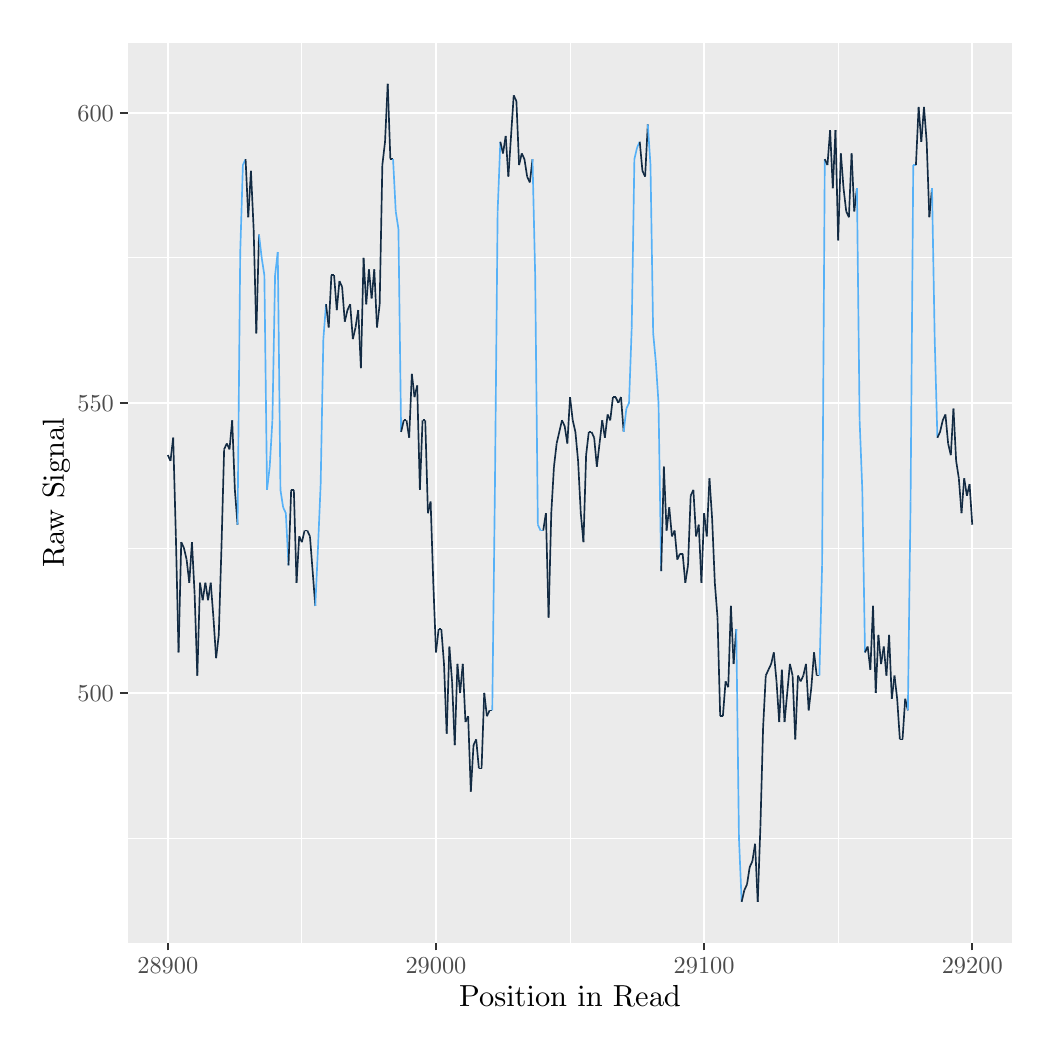
\begin{tikzpicture}[x=1pt,y=1pt]
\definecolor{fillColor}{RGB}{255,255,255}
\path[use as bounding box,fill=fillColor,fill opacity=0.00] (0,0) rectangle (361.35,361.35);
\begin{scope}
\path[clip] (  0.00,  0.00) rectangle (361.35,361.35);
\definecolor{drawColor}{RGB}{255,255,255}
\definecolor{fillColor}{RGB}{255,255,255}

\path[draw=drawColor,line width= 0.6pt,line join=round,line cap=round,fill=fillColor] (  0.00,  0.00) rectangle (361.35,361.35);
\end{scope}
\begin{scope}
\path[clip] ( 36.11, 30.69) rectangle (355.85,355.85);
\definecolor{fillColor}{gray}{0.92}

\path[fill=fillColor] ( 36.11, 30.69) rectangle (355.85,355.85);
\definecolor{drawColor}{RGB}{255,255,255}

\path[draw=drawColor,line width= 0.3pt,line join=round] ( 36.11, 68.53) --
	(355.85, 68.53);

\path[draw=drawColor,line width= 0.3pt,line join=round] ( 36.11,173.35) --
	(355.85,173.35);

\path[draw=drawColor,line width= 0.3pt,line join=round] ( 36.11,278.18) --
	(355.85,278.18);

\path[draw=drawColor,line width= 0.3pt,line join=round] ( 99.09, 30.69) --
	( 99.09,355.85);

\path[draw=drawColor,line width= 0.3pt,line join=round] (195.98, 30.69) --
	(195.98,355.85);

\path[draw=drawColor,line width= 0.3pt,line join=round] (292.87, 30.69) --
	(292.87,355.85);

\path[draw=drawColor,line width= 0.6pt,line join=round] ( 36.11,120.94) --
	(355.85,120.94);

\path[draw=drawColor,line width= 0.6pt,line join=round] ( 36.11,225.76) --
	(355.85,225.76);

\path[draw=drawColor,line width= 0.6pt,line join=round] ( 36.11,330.59) --
	(355.85,330.59);

\path[draw=drawColor,line width= 0.6pt,line join=round] ( 50.64, 30.69) --
	( 50.64,355.85);

\path[draw=drawColor,line width= 0.6pt,line join=round] (147.54, 30.69) --
	(147.54,355.85);

\path[draw=drawColor,line width= 0.6pt,line join=round] (244.43, 30.69) --
	(244.43,355.85);

\path[draw=drawColor,line width= 0.6pt,line join=round] (341.32, 30.69) --
	(341.32,355.85);
\definecolor{drawColor}{RGB}{19,43,67}

\path[draw=drawColor,line width= 0.6pt,line join=round] ( 50.64,206.90) -- ( 51.61,204.80);

\path[draw=drawColor,line width= 0.6pt,line join=round] ( 51.61,204.80) -- ( 52.58,213.18);

\path[draw=drawColor,line width= 0.6pt,line join=round] ( 52.58,213.18) -- ( 53.55,177.54);

\path[draw=drawColor,line width= 0.6pt,line join=round] ( 53.55,177.54) -- ( 54.52,135.61);

\path[draw=drawColor,line width= 0.6pt,line join=round] ( 54.52,135.61) -- ( 55.49,175.45);

\path[draw=drawColor,line width= 0.6pt,line join=round] ( 55.49,175.45) -- ( 56.46,173.35);

\path[draw=drawColor,line width= 0.6pt,line join=round] ( 56.46,173.35) -- ( 57.43,169.16);

\path[draw=drawColor,line width= 0.6pt,line join=round] ( 57.43,169.16) -- ( 58.40,160.77);

\path[draw=drawColor,line width= 0.6pt,line join=round] ( 58.40,160.77) -- ( 59.36,175.45);

\path[draw=drawColor,line width= 0.6pt,line join=round] ( 59.36,175.45) -- ( 60.33,156.58);

\path[draw=drawColor,line width= 0.6pt,line join=round] ( 60.33,156.58) -- ( 61.30,127.23);

\path[draw=drawColor,line width= 0.6pt,line join=round] ( 61.30,127.23) -- ( 62.27,160.77);

\path[draw=drawColor,line width= 0.6pt,line join=round] ( 62.27,160.77) -- ( 63.24,154.48);

\path[draw=drawColor,line width= 0.6pt,line join=round] ( 63.24,154.48) -- ( 64.21,160.77);

\path[draw=drawColor,line width= 0.6pt,line join=round] ( 64.21,160.77) -- ( 65.18,154.48);

\path[draw=drawColor,line width= 0.6pt,line join=round] ( 65.18,154.48) -- ( 66.15,160.77);

\path[draw=drawColor,line width= 0.6pt,line join=round] ( 66.15,160.77) -- ( 67.12,148.19);

\path[draw=drawColor,line width= 0.6pt,line join=round] ( 67.12,148.19) -- ( 68.09,133.52);

\path[draw=drawColor,line width= 0.6pt,line join=round] ( 68.09,133.52) -- ( 69.05,141.90);

\path[draw=drawColor,line width= 0.6pt,line join=round] ( 69.05,141.90) -- ( 70.02,173.35);

\path[draw=drawColor,line width= 0.6pt,line join=round] ( 70.02,173.35) -- ( 70.99,208.99);

\path[draw=drawColor,line width= 0.6pt,line join=round] ( 70.99,208.99) -- ( 71.96,211.09);

\path[draw=drawColor,line width= 0.6pt,line join=round] ( 71.96,211.09) -- ( 72.93,208.99);

\path[draw=drawColor,line width= 0.6pt,line join=round] ( 72.93,208.99) -- ( 73.90,219.47);

\path[draw=drawColor,line width= 0.6pt,line join=round] ( 73.90,219.47) -- ( 74.87,194.32);

\path[draw=drawColor,line width= 0.6pt,line join=round] ( 74.87,194.32) -- ( 75.84,181.74);
\definecolor{drawColor}{RGB}{86,177,247}

\path[draw=drawColor,line width= 0.6pt,line join=round] ( 75.84,181.74) -- ( 76.81,280.27);

\path[draw=drawColor,line width= 0.6pt,line join=round] ( 76.81,280.27) -- ( 77.77,311.72);

\path[draw=drawColor,line width= 0.6pt,line join=round] ( 77.77,311.72) -- ( 78.74,313.82);
\definecolor{drawColor}{RGB}{19,43,67}

\path[draw=drawColor,line width= 0.6pt,line join=round] ( 78.74,313.82) -- ( 79.71,292.85);

\path[draw=drawColor,line width= 0.6pt,line join=round] ( 79.71,292.85) -- ( 80.68,309.62);

\path[draw=drawColor,line width= 0.6pt,line join=round] ( 80.68,309.62) -- ( 81.65,288.66);

\path[draw=drawColor,line width= 0.6pt,line join=round] ( 81.65,288.66) -- ( 82.62,250.92);

\path[draw=drawColor,line width= 0.6pt,line join=round] ( 82.62,250.92) -- ( 83.59,286.56);
\definecolor{drawColor}{RGB}{86,177,247}

\path[draw=drawColor,line width= 0.6pt,line join=round] ( 83.59,286.56) -- ( 84.56,278.18);

\path[draw=drawColor,line width= 0.6pt,line join=round] ( 84.56,278.18) -- ( 85.53,271.89);

\path[draw=drawColor,line width= 0.6pt,line join=round] ( 85.53,271.89) -- ( 86.49,194.32);

\path[draw=drawColor,line width= 0.6pt,line join=round] ( 86.49,194.32) -- ( 87.46,202.70);

\path[draw=drawColor,line width= 0.6pt,line join=round] ( 87.46,202.70) -- ( 88.43,219.47);

\path[draw=drawColor,line width= 0.6pt,line join=round] ( 88.43,219.47) -- ( 89.40,271.89);

\path[draw=drawColor,line width= 0.6pt,line join=round] ( 89.40,271.89) -- ( 90.37,280.27);

\path[draw=drawColor,line width= 0.6pt,line join=round] ( 90.37,280.27) -- ( 91.34,194.32);

\path[draw=drawColor,line width= 0.6pt,line join=round] ( 91.34,194.32) -- ( 92.31,188.03);

\path[draw=drawColor,line width= 0.6pt,line join=round] ( 92.31,188.03) -- ( 93.28,185.93);

\path[draw=drawColor,line width= 0.6pt,line join=round] ( 93.28,185.93) -- ( 94.25,167.06);
\definecolor{drawColor}{RGB}{19,43,67}

\path[draw=drawColor,line width= 0.6pt,line join=round] ( 94.25,167.06) -- ( 95.21,194.32);

\path[draw=drawColor,line width= 0.6pt,line join=round] ( 95.21,194.32) -- ( 96.18,194.32);

\path[draw=drawColor,line width= 0.6pt,line join=round] ( 96.18,194.32) -- ( 97.15,160.77);

\path[draw=drawColor,line width= 0.6pt,line join=round] ( 97.15,160.77) -- ( 98.12,177.54);

\path[draw=drawColor,line width= 0.6pt,line join=round] ( 98.12,177.54) -- ( 99.09,175.45);

\path[draw=drawColor,line width= 0.6pt,line join=round] ( 99.09,175.45) -- (100.06,179.64);

\path[draw=drawColor,line width= 0.6pt,line join=round] (100.06,179.64) -- (101.03,179.64);

\path[draw=drawColor,line width= 0.6pt,line join=round] (101.03,179.64) -- (102.00,177.54);

\path[draw=drawColor,line width= 0.6pt,line join=round] (102.00,177.54) -- (102.97,164.97);

\path[draw=drawColor,line width= 0.6pt,line join=round] (102.97,164.97) -- (103.93,152.39);
\definecolor{drawColor}{RGB}{86,177,247}

\path[draw=drawColor,line width= 0.6pt,line join=round] (103.93,152.39) -- (104.90,173.35);

\path[draw=drawColor,line width= 0.6pt,line join=round] (104.90,173.35) -- (105.87,196.41);

\path[draw=drawColor,line width= 0.6pt,line join=round] (105.87,196.41) -- (106.84,248.82);

\path[draw=drawColor,line width= 0.6pt,line join=round] (106.84,248.82) -- (107.81,261.40);
\definecolor{drawColor}{RGB}{19,43,67}

\path[draw=drawColor,line width= 0.6pt,line join=round] (107.81,261.40) -- (108.78,253.02);

\path[draw=drawColor,line width= 0.6pt,line join=round] (108.78,253.02) -- (109.75,271.89);

\path[draw=drawColor,line width= 0.6pt,line join=round] (109.75,271.89) -- (110.72,271.89);

\path[draw=drawColor,line width= 0.6pt,line join=round] (110.72,271.89) -- (111.69,259.31);

\path[draw=drawColor,line width= 0.6pt,line join=round] (111.69,259.31) -- (112.65,269.79);

\path[draw=drawColor,line width= 0.6pt,line join=round] (112.65,269.79) -- (113.62,267.69);

\path[draw=drawColor,line width= 0.6pt,line join=round] (113.62,267.69) -- (114.59,255.11);

\path[draw=drawColor,line width= 0.6pt,line join=round] (114.59,255.11) -- (115.56,259.31);

\path[draw=drawColor,line width= 0.6pt,line join=round] (115.56,259.31) -- (116.53,261.40);

\path[draw=drawColor,line width= 0.6pt,line join=round] (116.53,261.40) -- (117.50,248.82);

\path[draw=drawColor,line width= 0.6pt,line join=round] (117.50,248.82) -- (118.47,253.02);

\path[draw=drawColor,line width= 0.6pt,line join=round] (118.47,253.02) -- (119.44,259.31);

\path[draw=drawColor,line width= 0.6pt,line join=round] (119.44,259.31) -- (120.41,238.34);

\path[draw=drawColor,line width= 0.6pt,line join=round] (120.41,238.34) -- (121.37,278.18);

\path[draw=drawColor,line width= 0.6pt,line join=round] (121.37,278.18) -- (122.34,261.40);

\path[draw=drawColor,line width= 0.6pt,line join=round] (122.34,261.40) -- (123.31,273.98);

\path[draw=drawColor,line width= 0.6pt,line join=round] (123.31,273.98) -- (124.28,263.50);

\path[draw=drawColor,line width= 0.6pt,line join=round] (124.28,263.50) -- (125.25,273.98);

\path[draw=drawColor,line width= 0.6pt,line join=round] (125.25,273.98) -- (126.22,253.02);

\path[draw=drawColor,line width= 0.6pt,line join=round] (126.22,253.02) -- (127.19,261.40);

\path[draw=drawColor,line width= 0.6pt,line join=round] (127.19,261.40) -- (128.16,311.72);

\path[draw=drawColor,line width= 0.6pt,line join=round] (128.16,311.72) -- (129.13,320.11);

\path[draw=drawColor,line width= 0.6pt,line join=round] (129.13,320.11) -- (130.10,341.07);

\path[draw=drawColor,line width= 0.6pt,line join=round] (130.10,341.07) -- (131.06,313.82);

\path[draw=drawColor,line width= 0.6pt,line join=round] (131.06,313.82) -- (132.03,313.82);
\definecolor{drawColor}{RGB}{86,177,247}

\path[draw=drawColor,line width= 0.6pt,line join=round] (132.03,313.82) -- (133.00,294.95);

\path[draw=drawColor,line width= 0.6pt,line join=round] (133.00,294.95) -- (133.97,288.66);

\path[draw=drawColor,line width= 0.6pt,line join=round] (133.97,288.66) -- (134.94,215.28);
\definecolor{drawColor}{RGB}{19,43,67}

\path[draw=drawColor,line width= 0.6pt,line join=round] (134.94,215.28) -- (135.91,219.47);

\path[draw=drawColor,line width= 0.6pt,line join=round] (135.91,219.47) -- (136.88,219.47);

\path[draw=drawColor,line width= 0.6pt,line join=round] (136.88,219.47) -- (137.85,213.18);

\path[draw=drawColor,line width= 0.6pt,line join=round] (137.85,213.18) -- (138.82,236.25);

\path[draw=drawColor,line width= 0.6pt,line join=round] (138.82,236.25) -- (139.78,227.86);

\path[draw=drawColor,line width= 0.6pt,line join=round] (139.78,227.86) -- (140.75,232.05);

\path[draw=drawColor,line width= 0.6pt,line join=round] (140.75,232.05) -- (141.72,194.32);

\path[draw=drawColor,line width= 0.6pt,line join=round] (141.72,194.32) -- (142.69,219.47);

\path[draw=drawColor,line width= 0.6pt,line join=round] (142.69,219.47) -- (143.66,219.47);

\path[draw=drawColor,line width= 0.6pt,line join=round] (143.66,219.47) -- (144.63,185.93);

\path[draw=drawColor,line width= 0.6pt,line join=round] (144.63,185.93) -- (145.60,190.12);

\path[draw=drawColor,line width= 0.6pt,line join=round] (145.60,190.12) -- (146.57,160.77);

\path[draw=drawColor,line width= 0.6pt,line join=round] (146.57,160.77) -- (147.54,135.61);

\path[draw=drawColor,line width= 0.6pt,line join=round] (147.54,135.61) -- (148.50,144.00);

\path[draw=drawColor,line width= 0.6pt,line join=round] (148.50,144.00) -- (149.47,144.00);

\path[draw=drawColor,line width= 0.6pt,line join=round] (149.47,144.00) -- (150.44,131.42);

\path[draw=drawColor,line width= 0.6pt,line join=round] (150.44,131.42) -- (151.41,106.26);

\path[draw=drawColor,line width= 0.6pt,line join=round] (151.41,106.26) -- (152.38,137.71);

\path[draw=drawColor,line width= 0.6pt,line join=round] (152.38,137.71) -- (153.35,125.13);

\path[draw=drawColor,line width= 0.6pt,line join=round] (153.35,125.13) -- (154.32,102.07);

\path[draw=drawColor,line width= 0.6pt,line join=round] (154.32,102.07) -- (155.29,131.42);

\path[draw=drawColor,line width= 0.6pt,line join=round] (155.29,131.42) -- (156.26,120.94);

\path[draw=drawColor,line width= 0.6pt,line join=round] (156.26,120.94) -- (157.22,131.42);

\path[draw=drawColor,line width= 0.6pt,line join=round] (157.22,131.42) -- (158.19,110.46);

\path[draw=drawColor,line width= 0.6pt,line join=round] (158.19,110.46) -- (159.16,112.55);

\path[draw=drawColor,line width= 0.6pt,line join=round] (159.16,112.55) -- (160.13, 85.30);

\path[draw=drawColor,line width= 0.6pt,line join=round] (160.13, 85.30) -- (161.10,102.07);

\path[draw=drawColor,line width= 0.6pt,line join=round] (161.10,102.07) -- (162.07,104.17);

\path[draw=drawColor,line width= 0.6pt,line join=round] (162.07,104.17) -- (163.04, 93.69);

\path[draw=drawColor,line width= 0.6pt,line join=round] (163.04, 93.69) -- (164.01, 93.69);

\path[draw=drawColor,line width= 0.6pt,line join=round] (164.01, 93.69) -- (164.98,120.94);

\path[draw=drawColor,line width= 0.6pt,line join=round] (164.98,120.94) -- (165.94,112.55);

\path[draw=drawColor,line width= 0.6pt,line join=round] (165.94,112.55) -- (166.91,114.65);

\path[draw=drawColor,line width= 0.6pt,line join=round] (166.91,114.65) -- (167.88,114.65);
\definecolor{drawColor}{RGB}{86,177,247}

\path[draw=drawColor,line width= 0.6pt,line join=round] (167.88,114.65) -- (168.85,196.41);

\path[draw=drawColor,line width= 0.6pt,line join=round] (168.85,196.41) -- (169.82,294.95);

\path[draw=drawColor,line width= 0.6pt,line join=round] (169.82,294.95) -- (170.79,320.11);
\definecolor{drawColor}{RGB}{19,43,67}

\path[draw=drawColor,line width= 0.6pt,line join=round] (170.79,320.11) -- (171.76,315.91);

\path[draw=drawColor,line width= 0.6pt,line join=round] (171.76,315.91) -- (172.73,322.20);

\path[draw=drawColor,line width= 0.6pt,line join=round] (172.73,322.20) -- (173.70,307.53);

\path[draw=drawColor,line width= 0.6pt,line join=round] (173.70,307.53) -- (174.66,322.20);

\path[draw=drawColor,line width= 0.6pt,line join=round] (174.66,322.20) -- (175.63,336.88);

\path[draw=drawColor,line width= 0.6pt,line join=round] (175.63,336.88) -- (176.60,334.78);

\path[draw=drawColor,line width= 0.6pt,line join=round] (176.60,334.78) -- (177.57,311.72);

\path[draw=drawColor,line width= 0.6pt,line join=round] (177.57,311.72) -- (178.54,315.91);

\path[draw=drawColor,line width= 0.6pt,line join=round] (178.54,315.91) -- (179.51,313.82);

\path[draw=drawColor,line width= 0.6pt,line join=round] (179.51,313.82) -- (180.48,307.53);

\path[draw=drawColor,line width= 0.6pt,line join=round] (180.48,307.53) -- (181.45,305.43);

\path[draw=drawColor,line width= 0.6pt,line join=round] (181.45,305.43) -- (182.42,313.82);
\definecolor{drawColor}{RGB}{86,177,247}

\path[draw=drawColor,line width= 0.6pt,line join=round] (182.42,313.82) -- (183.38,271.89);

\path[draw=drawColor,line width= 0.6pt,line join=round] (183.38,271.89) -- (184.35,181.74);

\path[draw=drawColor,line width= 0.6pt,line join=round] (184.35,181.74) -- (185.32,179.64);

\path[draw=drawColor,line width= 0.6pt,line join=round] (185.32,179.64) -- (186.29,179.64);
\definecolor{drawColor}{RGB}{19,43,67}

\path[draw=drawColor,line width= 0.6pt,line join=round] (186.29,179.64) -- (187.26,185.93);

\path[draw=drawColor,line width= 0.6pt,line join=round] (187.26,185.93) -- (188.23,148.19);

\path[draw=drawColor,line width= 0.6pt,line join=round] (188.23,148.19) -- (189.20,185.93);

\path[draw=drawColor,line width= 0.6pt,line join=round] (189.20,185.93) -- (190.17,202.70);

\path[draw=drawColor,line width= 0.6pt,line join=round] (190.17,202.70) -- (191.14,211.09);

\path[draw=drawColor,line width= 0.6pt,line join=round] (191.14,211.09) -- (192.10,215.28);

\path[draw=drawColor,line width= 0.6pt,line join=round] (192.10,215.28) -- (193.07,219.47);

\path[draw=drawColor,line width= 0.6pt,line join=round] (193.07,219.47) -- (194.04,217.38);

\path[draw=drawColor,line width= 0.6pt,line join=round] (194.04,217.38) -- (195.01,211.09);

\path[draw=drawColor,line width= 0.6pt,line join=round] (195.01,211.09) -- (195.98,227.86);

\path[draw=drawColor,line width= 0.6pt,line join=round] (195.98,227.86) -- (196.95,219.47);

\path[draw=drawColor,line width= 0.6pt,line join=round] (196.95,219.47) -- (197.92,215.28);

\path[draw=drawColor,line width= 0.6pt,line join=round] (197.92,215.28) -- (198.89,204.80);

\path[draw=drawColor,line width= 0.6pt,line join=round] (198.89,204.80) -- (199.86,185.93);

\path[draw=drawColor,line width= 0.6pt,line join=round] (199.86,185.93) -- (200.83,175.45);

\path[draw=drawColor,line width= 0.6pt,line join=round] (200.83,175.45) -- (201.79,206.90);

\path[draw=drawColor,line width= 0.6pt,line join=round] (201.79,206.90) -- (202.76,215.28);

\path[draw=drawColor,line width= 0.6pt,line join=round] (202.76,215.28) -- (203.73,215.28);

\path[draw=drawColor,line width= 0.6pt,line join=round] (203.73,215.28) -- (204.70,213.18);

\path[draw=drawColor,line width= 0.6pt,line join=round] (204.70,213.18) -- (205.67,202.70);

\path[draw=drawColor,line width= 0.6pt,line join=round] (205.67,202.70) -- (206.64,211.09);

\path[draw=drawColor,line width= 0.6pt,line join=round] (206.64,211.09) -- (207.61,219.47);

\path[draw=drawColor,line width= 0.6pt,line join=round] (207.61,219.47) -- (208.58,213.18);

\path[draw=drawColor,line width= 0.6pt,line join=round] (208.58,213.18) -- (209.55,221.57);

\path[draw=drawColor,line width= 0.6pt,line join=round] (209.55,221.57) -- (210.51,219.47);

\path[draw=drawColor,line width= 0.6pt,line join=round] (210.51,219.47) -- (211.48,227.86);

\path[draw=drawColor,line width= 0.6pt,line join=round] (211.48,227.86) -- (212.45,227.86);

\path[draw=drawColor,line width= 0.6pt,line join=round] (212.45,227.86) -- (213.42,225.76);

\path[draw=drawColor,line width= 0.6pt,line join=round] (213.42,225.76) -- (214.39,227.86);

\path[draw=drawColor,line width= 0.6pt,line join=round] (214.39,227.86) -- (215.36,215.28);
\definecolor{drawColor}{RGB}{86,177,247}

\path[draw=drawColor,line width= 0.6pt,line join=round] (215.36,215.28) -- (216.33,223.67);

\path[draw=drawColor,line width= 0.6pt,line join=round] (216.33,223.67) -- (217.30,225.76);

\path[draw=drawColor,line width= 0.6pt,line join=round] (217.30,225.76) -- (218.27,253.02);

\path[draw=drawColor,line width= 0.6pt,line join=round] (218.27,253.02) -- (219.23,313.82);

\path[draw=drawColor,line width= 0.6pt,line join=round] (219.23,313.82) -- (220.20,318.01);

\path[draw=drawColor,line width= 0.6pt,line join=round] (220.20,318.01) -- (221.17,320.11);
\definecolor{drawColor}{RGB}{19,43,67}

\path[draw=drawColor,line width= 0.6pt,line join=round] (221.17,320.11) -- (222.14,309.62);

\path[draw=drawColor,line width= 0.6pt,line join=round] (222.14,309.62) -- (223.11,307.53);

\path[draw=drawColor,line width= 0.6pt,line join=round] (223.11,307.53) -- (224.08,326.39);
\definecolor{drawColor}{RGB}{86,177,247}

\path[draw=drawColor,line width= 0.6pt,line join=round] (224.08,326.39) -- (225.05,311.72);

\path[draw=drawColor,line width= 0.6pt,line join=round] (225.05,311.72) -- (226.02,250.92);

\path[draw=drawColor,line width= 0.6pt,line join=round] (226.02,250.92) -- (226.99,240.44);

\path[draw=drawColor,line width= 0.6pt,line join=round] (226.99,240.44) -- (227.95,225.76);

\path[draw=drawColor,line width= 0.6pt,line join=round] (227.95,225.76) -- (228.92,164.97);
\definecolor{drawColor}{RGB}{19,43,67}

\path[draw=drawColor,line width= 0.6pt,line join=round] (228.92,164.97) -- (229.89,202.70);

\path[draw=drawColor,line width= 0.6pt,line join=round] (229.89,202.70) -- (230.86,179.64);

\path[draw=drawColor,line width= 0.6pt,line join=round] (230.86,179.64) -- (231.83,188.03);

\path[draw=drawColor,line width= 0.6pt,line join=round] (231.83,188.03) -- (232.80,177.54);

\path[draw=drawColor,line width= 0.6pt,line join=round] (232.80,177.54) -- (233.77,179.64);

\path[draw=drawColor,line width= 0.6pt,line join=round] (233.77,179.64) -- (234.74,169.16);

\path[draw=drawColor,line width= 0.6pt,line join=round] (234.74,169.16) -- (235.71,171.25);

\path[draw=drawColor,line width= 0.6pt,line join=round] (235.71,171.25) -- (236.67,171.25);

\path[draw=drawColor,line width= 0.6pt,line join=round] (236.67,171.25) -- (237.64,160.77);

\path[draw=drawColor,line width= 0.6pt,line join=round] (237.64,160.77) -- (238.61,167.06);

\path[draw=drawColor,line width= 0.6pt,line join=round] (238.61,167.06) -- (239.58,192.22);

\path[draw=drawColor,line width= 0.6pt,line join=round] (239.58,192.22) -- (240.55,194.32);

\path[draw=drawColor,line width= 0.6pt,line join=round] (240.55,194.32) -- (241.52,177.54);

\path[draw=drawColor,line width= 0.6pt,line join=round] (241.52,177.54) -- (242.49,181.74);

\path[draw=drawColor,line width= 0.6pt,line join=round] (242.49,181.74) -- (243.46,160.77);

\path[draw=drawColor,line width= 0.6pt,line join=round] (243.46,160.77) -- (244.43,185.93);

\path[draw=drawColor,line width= 0.6pt,line join=round] (244.43,185.93) -- (245.39,177.54);

\path[draw=drawColor,line width= 0.6pt,line join=round] (245.39,177.54) -- (246.36,198.51);

\path[draw=drawColor,line width= 0.6pt,line join=round] (246.36,198.51) -- (247.33,183.83);

\path[draw=drawColor,line width= 0.6pt,line join=round] (247.33,183.83) -- (248.30,160.77);

\path[draw=drawColor,line width= 0.6pt,line join=round] (248.30,160.77) -- (249.27,148.19);

\path[draw=drawColor,line width= 0.6pt,line join=round] (249.27,148.19) -- (250.24,112.55);

\path[draw=drawColor,line width= 0.6pt,line join=round] (250.24,112.55) -- (251.21,112.55);

\path[draw=drawColor,line width= 0.6pt,line join=round] (251.21,112.55) -- (252.18,125.13);

\path[draw=drawColor,line width= 0.6pt,line join=round] (252.18,125.13) -- (253.15,123.04);

\path[draw=drawColor,line width= 0.6pt,line join=round] (253.15,123.04) -- (254.11,152.39);

\path[draw=drawColor,line width= 0.6pt,line join=round] (254.11,152.39) -- (255.08,131.42);

\path[draw=drawColor,line width= 0.6pt,line join=round] (255.08,131.42) -- (256.05,144.00);
\definecolor{drawColor}{RGB}{86,177,247}

\path[draw=drawColor,line width= 0.6pt,line join=round] (256.05,144.00) -- (257.02, 68.53);

\path[draw=drawColor,line width= 0.6pt,line join=round] (257.02, 68.53) -- (257.99, 45.47);
\definecolor{drawColor}{RGB}{19,43,67}

\path[draw=drawColor,line width= 0.6pt,line join=round] (257.99, 45.47) -- (258.96, 49.66);

\path[draw=drawColor,line width= 0.6pt,line join=round] (258.96, 49.66) -- (259.93, 51.76);

\path[draw=drawColor,line width= 0.6pt,line join=round] (259.93, 51.76) -- (260.90, 58.04);

\path[draw=drawColor,line width= 0.6pt,line join=round] (260.90, 58.04) -- (261.87, 60.14);

\path[draw=drawColor,line width= 0.6pt,line join=round] (261.87, 60.14) -- (262.84, 66.43);

\path[draw=drawColor,line width= 0.6pt,line join=round] (262.84, 66.43) -- (263.80, 45.47);

\path[draw=drawColor,line width= 0.6pt,line join=round] (263.80, 45.47) -- (264.77, 72.72);

\path[draw=drawColor,line width= 0.6pt,line join=round] (264.77, 72.72) -- (265.74,108.36);

\path[draw=drawColor,line width= 0.6pt,line join=round] (265.74,108.36) -- (266.71,127.23);

\path[draw=drawColor,line width= 0.6pt,line join=round] (266.71,127.23) -- (267.68,129.33);

\path[draw=drawColor,line width= 0.6pt,line join=round] (267.68,129.33) -- (268.65,131.42);

\path[draw=drawColor,line width= 0.6pt,line join=round] (268.65,131.42) -- (269.62,135.61);

\path[draw=drawColor,line width= 0.6pt,line join=round] (269.62,135.61) -- (270.59,125.13);

\path[draw=drawColor,line width= 0.6pt,line join=round] (270.59,125.13) -- (271.56,110.46);

\path[draw=drawColor,line width= 0.6pt,line join=round] (271.56,110.46) -- (272.52,129.33);

\path[draw=drawColor,line width= 0.6pt,line join=round] (272.52,129.33) -- (273.49,110.46);

\path[draw=drawColor,line width= 0.6pt,line join=round] (273.49,110.46) -- (274.46,120.94);

\path[draw=drawColor,line width= 0.6pt,line join=round] (274.46,120.94) -- (275.43,131.42);

\path[draw=drawColor,line width= 0.6pt,line join=round] (275.43,131.42) -- (276.40,127.23);

\path[draw=drawColor,line width= 0.6pt,line join=round] (276.40,127.23) -- (277.37,104.17);

\path[draw=drawColor,line width= 0.6pt,line join=round] (277.37,104.17) -- (278.34,127.23);

\path[draw=drawColor,line width= 0.6pt,line join=round] (278.34,127.23) -- (279.31,125.13);

\path[draw=drawColor,line width= 0.6pt,line join=round] (279.31,125.13) -- (280.28,127.23);

\path[draw=drawColor,line width= 0.6pt,line join=round] (280.28,127.23) -- (281.24,131.42);

\path[draw=drawColor,line width= 0.6pt,line join=round] (281.24,131.42) -- (282.21,114.65);

\path[draw=drawColor,line width= 0.6pt,line join=round] (282.21,114.65) -- (283.18,123.04);

\path[draw=drawColor,line width= 0.6pt,line join=round] (283.18,123.04) -- (284.15,135.61);

\path[draw=drawColor,line width= 0.6pt,line join=round] (284.15,135.61) -- (285.12,127.23);

\path[draw=drawColor,line width= 0.6pt,line join=round] (285.12,127.23) -- (286.09,127.23);
\definecolor{drawColor}{RGB}{86,177,247}

\path[draw=drawColor,line width= 0.6pt,line join=round] (286.09,127.23) -- (287.06,167.06);

\path[draw=drawColor,line width= 0.6pt,line join=round] (287.06,167.06) -- (288.03,313.82);
\definecolor{drawColor}{RGB}{19,43,67}

\path[draw=drawColor,line width= 0.6pt,line join=round] (288.03,313.82) -- (289.00,311.72);

\path[draw=drawColor,line width= 0.6pt,line join=round] (289.00,311.72) -- (289.96,324.30);

\path[draw=drawColor,line width= 0.6pt,line join=round] (289.96,324.30) -- (290.93,303.33);

\path[draw=drawColor,line width= 0.6pt,line join=round] (290.93,303.33) -- (291.90,324.30);

\path[draw=drawColor,line width= 0.6pt,line join=round] (291.90,324.30) -- (292.87,284.46);

\path[draw=drawColor,line width= 0.6pt,line join=round] (292.87,284.46) -- (293.84,315.91);

\path[draw=drawColor,line width= 0.6pt,line join=round] (293.84,315.91) -- (294.81,303.33);

\path[draw=drawColor,line width= 0.6pt,line join=round] (294.81,303.33) -- (295.78,294.95);

\path[draw=drawColor,line width= 0.6pt,line join=round] (295.78,294.95) -- (296.75,292.85);

\path[draw=drawColor,line width= 0.6pt,line join=round] (296.75,292.85) -- (297.72,315.91);

\path[draw=drawColor,line width= 0.6pt,line join=round] (297.72,315.91) -- (298.68,294.95);

\path[draw=drawColor,line width= 0.6pt,line join=round] (298.68,294.95) -- (299.65,303.33);
\definecolor{drawColor}{RGB}{86,177,247}

\path[draw=drawColor,line width= 0.6pt,line join=round] (299.65,303.33) -- (300.62,219.47);

\path[draw=drawColor,line width= 0.6pt,line join=round] (300.62,219.47) -- (301.59,194.32);

\path[draw=drawColor,line width= 0.6pt,line join=round] (301.59,194.32) -- (302.56,135.61);
\definecolor{drawColor}{RGB}{19,43,67}

\path[draw=drawColor,line width= 0.6pt,line join=round] (302.56,135.61) -- (303.53,137.71);

\path[draw=drawColor,line width= 0.6pt,line join=round] (303.53,137.71) -- (304.50,129.33);

\path[draw=drawColor,line width= 0.6pt,line join=round] (304.50,129.33) -- (305.47,152.39);

\path[draw=drawColor,line width= 0.6pt,line join=round] (305.47,152.39) -- (306.44,120.94);

\path[draw=drawColor,line width= 0.6pt,line join=round] (306.44,120.94) -- (307.40,141.90);

\path[draw=drawColor,line width= 0.6pt,line join=round] (307.40,141.90) -- (308.37,131.42);

\path[draw=drawColor,line width= 0.6pt,line join=round] (308.37,131.42) -- (309.34,137.71);

\path[draw=drawColor,line width= 0.6pt,line join=round] (309.34,137.71) -- (310.31,127.23);

\path[draw=drawColor,line width= 0.6pt,line join=round] (310.31,127.23) -- (311.28,141.90);

\path[draw=drawColor,line width= 0.6pt,line join=round] (311.28,141.90) -- (312.25,118.84);

\path[draw=drawColor,line width= 0.6pt,line join=round] (312.25,118.84) -- (313.22,127.23);

\path[draw=drawColor,line width= 0.6pt,line join=round] (313.22,127.23) -- (314.19,118.84);

\path[draw=drawColor,line width= 0.6pt,line join=round] (314.19,118.84) -- (315.16,104.17);

\path[draw=drawColor,line width= 0.6pt,line join=round] (315.16,104.17) -- (316.12,104.17);

\path[draw=drawColor,line width= 0.6pt,line join=round] (316.12,104.17) -- (317.09,118.84);

\path[draw=drawColor,line width= 0.6pt,line join=round] (317.09,118.84) -- (318.06,114.65);
\definecolor{drawColor}{RGB}{86,177,247}

\path[draw=drawColor,line width= 0.6pt,line join=round] (318.06,114.65) -- (319.03,190.12);

\path[draw=drawColor,line width= 0.6pt,line join=round] (319.03,190.12) -- (320.00,311.72);

\path[draw=drawColor,line width= 0.6pt,line join=round] (320.00,311.72) -- (320.97,311.72);
\definecolor{drawColor}{RGB}{19,43,67}

\path[draw=drawColor,line width= 0.6pt,line join=round] (320.97,311.72) -- (321.94,332.68);

\path[draw=drawColor,line width= 0.6pt,line join=round] (321.94,332.68) -- (322.91,320.11);

\path[draw=drawColor,line width= 0.6pt,line join=round] (322.91,320.11) -- (323.88,332.68);

\path[draw=drawColor,line width= 0.6pt,line join=round] (323.88,332.68) -- (324.85,320.11);

\path[draw=drawColor,line width= 0.6pt,line join=round] (324.85,320.11) -- (325.81,292.85);

\path[draw=drawColor,line width= 0.6pt,line join=round] (325.81,292.85) -- (326.78,303.33);
\definecolor{drawColor}{RGB}{86,177,247}

\path[draw=drawColor,line width= 0.6pt,line join=round] (326.78,303.33) -- (327.75,248.82);

\path[draw=drawColor,line width= 0.6pt,line join=round] (327.75,248.82) -- (328.72,213.18);
\definecolor{drawColor}{RGB}{19,43,67}

\path[draw=drawColor,line width= 0.6pt,line join=round] (328.72,213.18) -- (329.69,215.28);

\path[draw=drawColor,line width= 0.6pt,line join=round] (329.69,215.28) -- (330.66,219.47);

\path[draw=drawColor,line width= 0.6pt,line join=round] (330.66,219.47) -- (331.63,221.57);

\path[draw=drawColor,line width= 0.6pt,line join=round] (331.63,221.57) -- (332.60,211.09);

\path[draw=drawColor,line width= 0.6pt,line join=round] (332.60,211.09) -- (333.57,206.90);

\path[draw=drawColor,line width= 0.6pt,line join=round] (333.57,206.90) -- (334.53,223.67);

\path[draw=drawColor,line width= 0.6pt,line join=round] (334.53,223.67) -- (335.50,204.80);

\path[draw=drawColor,line width= 0.6pt,line join=round] (335.50,204.80) -- (336.47,198.51);

\path[draw=drawColor,line width= 0.6pt,line join=round] (336.47,198.51) -- (337.44,185.93);

\path[draw=drawColor,line width= 0.6pt,line join=round] (337.44,185.93) -- (338.41,198.51);

\path[draw=drawColor,line width= 0.6pt,line join=round] (338.41,198.51) -- (339.38,192.22);

\path[draw=drawColor,line width= 0.6pt,line join=round] (339.38,192.22) -- (340.35,196.41);

\path[draw=drawColor,line width= 0.6pt,line join=round] (340.35,196.41) -- (341.32,181.74);
\end{scope}
\begin{scope}
\path[clip] (  0.00,  0.00) rectangle (361.35,361.35);
\definecolor{drawColor}{gray}{0.30}

\node[text=drawColor,anchor=base east,inner sep=0pt, outer sep=0pt, scale=  0.88] at ( 31.16,117.91) {500};

\node[text=drawColor,anchor=base east,inner sep=0pt, outer sep=0pt, scale=  0.88] at ( 31.16,222.73) {550};

\node[text=drawColor,anchor=base east,inner sep=0pt, outer sep=0pt, scale=  0.88] at ( 31.16,327.56) {600};
\end{scope}
\begin{scope}
\path[clip] (  0.00,  0.00) rectangle (361.35,361.35);
\definecolor{drawColor}{gray}{0.20}

\path[draw=drawColor,line width= 0.6pt,line join=round] ( 33.36,120.94) --
	( 36.11,120.94);

\path[draw=drawColor,line width= 0.6pt,line join=round] ( 33.36,225.76) --
	( 36.11,225.76);

\path[draw=drawColor,line width= 0.6pt,line join=round] ( 33.36,330.59) --
	( 36.11,330.59);
\end{scope}
\begin{scope}
\path[clip] (  0.00,  0.00) rectangle (361.35,361.35);
\definecolor{drawColor}{gray}{0.20}

\path[draw=drawColor,line width= 0.6pt,line join=round] ( 50.64, 27.94) --
	( 50.64, 30.69);

\path[draw=drawColor,line width= 0.6pt,line join=round] (147.54, 27.94) --
	(147.54, 30.69);

\path[draw=drawColor,line width= 0.6pt,line join=round] (244.43, 27.94) --
	(244.43, 30.69);

\path[draw=drawColor,line width= 0.6pt,line join=round] (341.32, 27.94) --
	(341.32, 30.69);
\end{scope}
\begin{scope}
\path[clip] (  0.00,  0.00) rectangle (361.35,361.35);
\definecolor{drawColor}{gray}{0.30}

\node[text=drawColor,anchor=base,inner sep=0pt, outer sep=0pt, scale=  0.88] at ( 50.64, 19.68) {28900};

\node[text=drawColor,anchor=base,inner sep=0pt, outer sep=0pt, scale=  0.88] at (147.54, 19.68) {29000};

\node[text=drawColor,anchor=base,inner sep=0pt, outer sep=0pt, scale=  0.88] at (244.43, 19.68) {29100};

\node[text=drawColor,anchor=base,inner sep=0pt, outer sep=0pt, scale=  0.88] at (341.32, 19.68) {29200};
\end{scope}
\begin{scope}
\path[clip] (  0.00,  0.00) rectangle (361.35,361.35);
\definecolor{drawColor}{RGB}{0,0,0}

\node[text=drawColor,anchor=base,inner sep=0pt, outer sep=0pt, scale=  1.10] at (195.98,  7.64) {Position in Read};
\end{scope}
\begin{scope}
\path[clip] (  0.00,  0.00) rectangle (361.35,361.35);
\definecolor{drawColor}{RGB}{0,0,0}

\node[text=drawColor,rotate= 90.00,anchor=base,inner sep=0pt, outer sep=0pt, scale=  1.10] at ( 13.08,193.27) {Raw Signal};
\end{scope}
\end{tikzpicture}

\caption{\label{fig:epsilon-25}300 data points from a DNA section in the read with ID e9f08690-171f-476f-9119-5330d0290126. The jumps and falls are highlighted for $\epsilon=24$.}
\end{figure}



\subsubsection{Subsequence Searching}
Some of the previously discussed compression methods, such as bit packing and FOR, depend on global statistics of the data such as the minimum and maximum.
For nanopore signal data, these statistics are easily dominated by outliers in the data.
One naive solution is to separately compress adjacent subsequences of equal length.
This approach has previously been successful in the literature with methods such as SIMD-BP128 and fast patched frame-of-reference (FastPFOR) performing compression in blocks of 128 integers \cite{lemire-simd}.

% Explore blocks of different sizes
% Explore blocks of different equal splits

Consider partitioning the nanopore signal into adjacent variable length blocks.
Let $P(x,s)$ be the partitioning of signal $x$ into $|s|=m\ge 1$ partitions according to partitioner $s$ where
\[ s := (s_j \in \mathbb{Z}\cap [0, n) \mid s_0 = 0)\]
and $s_j$ is the starting index of the $j$-th partition such that
\[ P(x,s) = (p_j) := ((x_{s_j},x_{s_j+1},\dots,x_{s_{j+1}-1}))_{j\in\mathbb{Z}\cap[0,m)}.\]
% TODO this is not correct for the last partition
%((x_{s_0},x_{s_0+1},\dots,x_{s_1-1}),(x_{s_1},\dots,x_{s_2-1}),\dots,(x_{s_{m-1}},\dots,x_n)) .\]
For example, if $x=(656,527,515,527,526)$ and $s = (0,3,4)$ then $m=3$ and
\[P(x,s)=((656,527,515),(527),(526)).\]

Given the partitioning $P$ we would like to compress each partition $p_j$ separately and concatenate the results.
Let $M(p)$ be the compressed bytes of partition $p$ after applying compression method $M$.
Then, the compressed bytes of signal $x$ under partitioner $s$ is the concatenation of the compressed bytes of each partition $M(p_j)$ given by
\[ C(x,s,M) := (M(p_j)\mid p_j=P(x,s)_j). \]
Let $\hat s$ be the partitioner of $x$ which minimises the number of compressed bytes
\[ |C(x,\hat s,M)| = \min_s |C(x,s,M)| = \min_s \sum_j|M(p_j)|. \]
The minimum number of compressed bytes can be found using the following recursive relationship
\begin{align*}
	|C(x,\hat s,M)| &= M(x) & n = 1\\
	|C(x,\hat s,M)| &= \min\{M(x),\min_{0\le k\le n-2}\{|C(x_L,\hat s_{x_L},M)| + |C(x_R,\hat s_{x_R},M)|\}\} & n\ge 2
\end{align*}
where $x_L=(x_0,x_1,\dots,x_k)$ and $x_R=(x_{k+1},\dots,x_{n-1})$.
That is, the compressed bytes with minimum length are found by either compressing the whole signal as usual or by dividing the signal into two partitions and concatenating each partition's minimum length compressed bytes.

For a signal of size $n$, the number of comparisons is given by the recurrence relation
\begin{align*}
	c_1 &= c_{M,1}\\
	c_n &= c_{M,n} + \sum_{k=0}^{n-2}(c_{k+1}+c_{n-k-1} + 1) &n\ge 2
	%TODO +1 for adding?
\end{align*}
where $c_{M,n}$ is the number of comparisons for the compression method $M$ on input size $n$.
This can be simplified as follows
\begin{align*}
	c_n &= c_{M,n} + \sum_{k=1}^{n-1}(2c_k + 1)\\
	&= c_{M,n} + n-1 + 2\sum_{k=1}^{n-1}c_k &n\ge 2
\end{align*}
Let's write $c_n$ in terms of $c_{n-1}$ in order to solve the recurrence more easily.
\begin{align*}
	c_{n-1} &= c_{M,n-1} + n - 2 + 2\sum_{k=1}^{n-2}c_k & n\ge 3\\
	c_{n} - c_{n-1} &= c_{M,n} - c_{M,n-1} + 1 + 2c_{n-1} \\
	c_{n} &= c_{M,n} - c_{M,n-1} + 1 + 3c_{n-1} & n\ge 2
\end{align*}
%TODO cite formula here?
Unrolling this we find that
\begin{align*}
	c_n &= c_{M,n} + \sum_{k=1}^{n-1}3^{k-1}(2c_{M,n-k} + 1) & n\ge 2.
\end{align*}
If the compression method has linear time complexity (i.e. $c_{M,n} = O(n)$) then
\begin{align*}
	c_n &= O(n) + \sum_{k=1}^{n-1}3^{k-1}(2O(n-k) + 1)\\
	&= O(n) + \sum_{k=1}^{n-1}3^{k-1}O(n-k)\\
	&= O(3^n) & \text{See Appendix \ref{app:cn}}
\end{align*}
That is, it takes exponential time to find the minimum compressed size using the naive recursive algorithm.
%TODO why different to subsequence sum

However, this algorithm re-computes the compressed bytes of subsequences many times rather than calculating it once and caching the data.
A better approach is to use bottom-up dynamic programming which avoids recursion and hence stack overflows.
The approach would compute the minimum number of compressed bytes for all subsequences of length $1$ then $2$, $3$ and so forth up to $n$. The results are stored in a triangular matrix $OPT\in \mathbb{N}\times\mathbb{N}$ where $OPT_{i,j}$ is the minimum number of compressed bytes of the subsequence starting at index $i$ and ending at index $j$.
It is triangular since we are not interested in subsequences which end before they begin. That is, we require that $i\le j$.

%TODO put algorithm here

For a signal of size $n$, the algorithm has the following number of comparisons
\[ \tilde c_n = \sum_{k=1}^n(n-k+1)(c_{M,k}+k-1) \]
since there are $n-k+1$ subsequences of size $k$ and each must compare compressing itself to concatenating $k-1$ pairs of compressed subdivisions.
Suppose as before that the compression method takes linear time. Then $\tilde c_n$ simplifies to
\begin{align*}
	\tilde c_n &= \sum_{k=1}^n(n-k+1)(O(k)+k-1)\\
	&= \sum_{k=1}^n(n-k+1)O(k)\\
	&= O(n^3) &\text{See Appendix \ref{app:cn-dyn}}
\end{align*}
Interestingly, $c_n$ and $\tilde c_n$ are asymptotically related by having opposite base and power terms; 3 and $n$.

%What is the length of these subsequences?

We can speed up the algorithm without a significant loss in compression by ignoring subsequences smaller than $l$ and moving between subsequence lengths at a step of $\delta_1$ and subsequences of the same length at a step of $\delta_2$.
The idea is that for compression method $M$, there exists some $l$ such that the minimum number of compressed bytes of subsequence $y$ with size $|y|<l$ equals the number of regular compressed bytes of $y$ with high probability.
In mathematical notation $\exists l\in\mathbb{N}^+$ such that $\forall x,\;|x|<l$
\[ P(C(x,\hat s,M)=M(x))> 1-\epsilon\]
for small $\epsilon \le 0.05$.
Furthermore, it is not necessary to calculate subsequences of all lengths or all subsequences of the same length since subsequences which differ by a couple signals should not provide a significantly better partition. This is because the deltas between successive signal values are small.
Rather, we want to calculate the minimum number of compressed bytes for subsequences of length $l,l+\delta_1,l+2\delta_1,\dots,l + \lfloor\frac{n-l}{\delta_1}\rfloor\delta_1, n$.
Then for subsequences of a particular length $p$ we calculate the minimum number of compressed bytes for subsequences $\delta_2$ apart, of the form $(x_{i\delta_2},x_{1+i\delta_2},\dots,x_{p-1+ i\delta_2})$ where $0\le i\le \lfloor \frac{n-p}{\delta_2} \rfloor$.

%TODO put algorithm here

For a signal of size $n$, the algorithm now has the following number of comparisons
%\[ \tilde c_n = \sum_{k=l}^n(n-k+1)(c_{M,k}+k-1) \]

However, we can exploit the characteristics of nanopore signal data to find better subsequences.
For example, each read typically consists of a stall.

%The next idea is to divide $x$ into subsequences with small range and compress each subsequence separately.
%Let $OPT(i, j)$ be the minimum number of bytes after compressing $(x_i,\dots, x_j)$. Then,
%\[ OPT(i, j) = \min(bytes(i, j),\min_{i\le k<j}(OPT(i, k) + OPT(k+1, j))) \]


\section{Other}
% Explore integer methods without generic

Instead, each integer can be represented more space-efficiently by using $b<16$ bits where \[b(x)=\lceil\log_2(\max(x))\rceil.\] In this case, the compression ratio would be approximately $16/b$:
\begin{align*}
	\text{Compression Ratio} &= \frac{\text{Uncompressed Bytes}}{\text{Compressed Bytes}}\\
	&=\frac{\frac{16}{8}n}{\lceil\frac{b}{8}n\rceil}\\
	&\stackrel{n\to\infty}{\longrightarrow}\frac{16}{b}.
\end{align*}
A better strategy would be to initially transform the data such that its range is decreased.
%Let \[T=\{t\mid t:X\to Y\}\] be the set of bijections from $X$, the set of reads, to $Y := \{(y_i\mid y_i\in \mathbb{N}_0)\}$. One such transformation is defined by
Let \[T=\{t\mid t:X\to X\}\] be the set of functions from $X$, the set of reads, to itself. One such transformation subtracts the minimum of $x$ from each integer and is defined by \[ submin(x) := (x_i-\min(x)). \] Each transformed integer can then be represented using fewer than or the same number of bits:
%A better strategy would be to first transform $x$ by subtracting the minimum of $x$ from each integer. That is, $x\mapsto(x_i-\min(x))$. Then,
\begin{align*}
	b(submin(x))&=\lceil\log_2(\max(submin(x)))\rceil\\
	&=\lceil\log_2(\max(x-\min(x)))\rceil\\
	&=\lceil\log_2(\max(x)-\min(x))\rceil\\
	&\le b(x)
\end{align*}
since $\log$ is an increasing function.
%However, in practice each integer lies within $[2^7,2^{11}]$. This means each integer can be represented using 11 bits rather than 16. If each integer is stored using $b$ bits, the compression ratio would be approximately $16/b$ as follows:
%Hence, using 11 bits per integer results in a compression ratio of approximately $1.\overline{45}$. Note that the optimal $b$ is given by
Another transformation takes the differences between successive signals and is defined by
\[ \delta(x):=(x_{i+1}-x_i\mid 0\le i\le n-2).\]

